\documentclass[11pt,a4paper,twoside]{bayesxreport}

\usepackage{amsfonts}
\usepackage[dvips]{graphicx}
\usepackage[dvips]{epsfig}
\usepackage{fancyhdr}

%\usepackage{showkeys}
%\usepackage{showidx}

\usepackage{rotating}
\usepackage{shortvrb}
\usepackage{multicol}
\usepackage{xr}

\usepackage[ps2pdf]{thumbpdf}
\usepackage[ps2pdf]{hyperref}
\hypersetup{
%    pdffitwindow=true,
    pdfstartview=FitB,
    pdftitle={BayesX Reference Manual},
    pdfauthor={Andreas Brezger, Thomas Kneib and Stefan Lang with contributions
    by Christiane Belitz, Eva-Maria Fronk, Andrea Hennerfeind,
    Petra Kragler, Manuela Hummel and Leyre Osuna Echavarr\'{\i}a},
    colorlinks=true,
    linkcolor=blue,
    pdfpagemode=UseOutlines,
    bookmarksopen=true,
    bookmarksnumbered=true,
    pdfstartpage={1},
    hyperindex=true
    }

\sloppy
\parindent0em
\parskip0.3em
\topmargin -0.3cm \textheight24cm \textwidth16.5cm \headheight0.5cm
\oddsidemargin-0.4cm \evensidemargin-0.4cm

 \fancyhead[RO,LE]{\thepage}
 \fancyhead[C]{}
 \fancyhead[LO]{\nouppercase\rightmark}
 \fancyhead[RE]{\nouppercase\leftmark}
 \fancyfoot[RO,LE]{}
 \fancyfoot[C]{\small\today} %Am ende raus!!!
 \fancyfoot[LO,RE]{}
 \fancyfoot[C]{}

 \renewcommand{\headrulewidth}{.4pt}
 \renewcommand{\footrulewidth}{0pt} %Am Ende 0 !!!
 \renewcommand{\chaptername}{Tutorial}

\pagestyle{fancy}


\renewcommand{\descriptionlabel}[1]{\hspace\labelsep\sc #1}

\def \re {{\bf R}}
\def \beq {\begin{equation}}
\def \eeq {\end{equation}}
\def \bdis {\begin{displaymath}}
\def \edis {\end{displaymath}}
\def \ds {\displaystyle}

\def \mbeta {\mbox{\boldmath $\beta$}}
\def \mtheta {\mbox{\boldmath $\theta$}}
\def \hatmbeta {\mbox{\boldmath $\hat\beta$}}
\def \eps {\epsilon}
\def \meps {\mbox{\boldmath $\epsilon$}}
\def \mmu {\mbox{\boldmath $\mu$}}
\def \mnu {\mbox{\boldmath $\nu$}}
\def \mSigma {\mbox{\boldmath $\Sigma$}}
\def \mGamma {\mbox{\boldmath $\Gamma$}}
\def \msigma {\mbox{\boldmath $\sigma$}}
\def \mPhi {\mbox{\boldmath $\Phi$}}

\newcommand{\N}{\mbox{N}}
\newcommand{\Var}{\mbox{Var}}
\newcommand{\E}{\mbox{E}}

\newcommand{\X}{\mbox{\boldmath $X$}}
\newcommand{\x}{\mbox{\boldmath $x$}}
\newcommand{\Z}{\mbox{\boldmath $Z$}}
\newcommand{\z}{\mbox{\boldmath $z$}}
\newcommand{\mb}{\mbox{\boldmath $b$}}
\newcommand{\Fx}{\mbox{\scriptsize \boldmath $x$}}
\newcommand{\I}{\mbox{\boldmath $I$}}
\newcommand{\Y}{\mbox{\boldmath $Y$}}
\newcommand{\y}{\mbox{\boldmath $y$}}
\newcommand{\mS}{\mbox{\boldmath $S$}}
\newcommand{\T}{\mbox{\boldmath $T$}}
\newcommand{\K}{\mbox{\boldmath $K$}}
\newcommand{\kt}{\mbox{\boldmath $t$}}
\newcommand{\U}{\mbox{\boldmath $U$}}
\newcommand{\fu}{\mbox{\boldmath $u$}}
\newcommand{\ba}{\mbox{\boldmath $\alpha$}}
\newcommand{\bb}{\mbox{\boldmath $\beta$}}

\newcommand{\subheader}[1]{\textsf{\textbf{{\large #1}}}}

\newenvironment{stanza}[2]{\subheader{#1} \begin{itemize} \item[]#2}{\end{itemize}}

 \externaldocument{manual}
 \externaldocument{manual_star}

\makeindex

\begin{document}
\MakeShortVerb{\#}

\thispagestyle{empty}

\begin{center}
{\bf \em \huge Bayes{\Huge X}}

\vspace{0.5cm}

{\em \large Software for Bayesian Inference}

\vspace{0.5cm}

{\em Version 1.30}

\vspace{0.5cm}

\begin{figure}[h]
\begin{center}
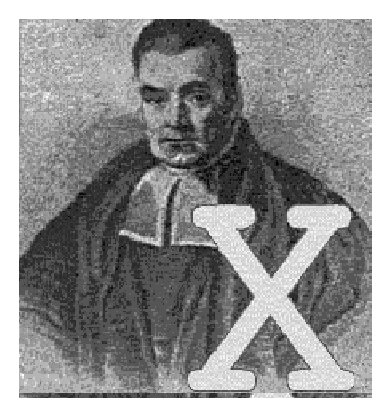
\includegraphics[scale=1.2]{grafiken/bayesicon.eps}
\end{center}
\end{figure}

\vfill

{\bf\sffamily \huge Tutorials}

\vfill

\end{center}

\begin{table}[ht]
\begin{center}
\begin{tabular}{lll}
{\em developed at} & \hspace{1.5cm} & {\em developed by} \\
University of Munich & \hspace{1.5cm} & Andreas Brezger \\
Department of Statistics & \hspace{1.5cm} & Thomas Kneib \\
Ludwigstr. 33 & \hspace{1.5cm} & Stefan Lang \\
80539 Munich & \hspace{1.5cm} & \\
  & & \\
{\em with contributions by}  &  \hspace{1.5cm} &  {\em supported by} \\
Christiane Belitz&  \hspace{1.5cm} & Ludwig Fahrmeir (mentally) \\
Eva--Maria Fronk  & \hspace{1.5cm} & Leo Held (mentally) \\
Andrea Hennerfeind & \hspace{1.5cm} & German Science Foundation  \\
Manuela Hummel & \\
Alexander Jerak & \\
Petra Kragler & \\
Leyre Osuna Echavarr\'{\i}a& \\
\end{tabular}
\end{center}
\end{table}


\newpage

\subsection*{Acknowledgements}

The development of {\em BayesX} has been supported by grants from
the German National Science Foundation (DFG),
Sonderforschungsbereich 386.

Special thanks go to (in alphabetical order of first names):

{\em Dieter Gollnow} for computing and providing the map of Munich (a really hard job); \\
{\em Leo Held} for advertising the program; \\
{\em Ludwig Fahrmeir} for his patience with finishing the program
and for carefully
reading and correcting the  manual; \\
{\em Ngianga-Bakwin Kandala} for being the first user of the program (a really hard job); \\
{\em Samson Babatunde Adebayo} for carefully reading and correcting the manual; \\
{\em Ursula Becker} for carefully reading and correcting the manual;

\subsection*{Licensing agreement} The authors of this software grant
to any individual or non-commercial organization the right to use
and to make an unlimited number of copies of this software. Usage by
commercial entities requires a license from the authors. You may not
decompile, disassemble, reverse engineer, or modify the software.
This includes, but is not limited to modifying/changing any icons,
menus, or displays associated with the software. This software
cannot be sold without written authorization from the authors. This
restriction is not intended to apply for connect time charges, or
flat rate connection/download fees for electronic bulletin board
services. The authors of this program accept no responsibility for
damages resulting from the use of this software and make no warranty
on representation, either express or implied, including but not
limited to, any implied warranty of merchantability or fitness for a
particular purpose. This software is provided as is, and you, its
user, assume all risks when using it.

\vspace{0.5cm}

{\em BayesX} is available at {
\href{http://www.stat.uni-muenchen.de/~bayesx}{http://www.stat.uni-muenchen.de/\~{}bayesx}}

\newpage

\chapter[A tutorial
on Bayesian semiparametric regression using MCMC
techniques]{Determinants of childhood undernutrition in Zambia: A
tutorial on Bayesian semiparametric regression using MCMC
techniques} \label{zambiaanalysis}

In this chapter we present a tutorial like example for the usage of
{\em bayesreg objects}. We use data on undernutrition of children in
Zambia, compare \autoref{zambia} for a description of the data set.
The files containing the data and the map can be found in the
subdirectory #examples# of the installation directory together with
the batch file #mcmctutorial.prg# containing all commands used in
the following subsections.

The rest of the example is separated in seven parts dealing with the
different steps of estimating a regression model. In
\autoref{zambia_mcmc_datasets} we create a {\em dataset object} to
incorporate, handle and manipulate the data. We will also give a
brief description of some methods that may be applied to {\em
dataset objects}. Since we want to estimate a spatial effect of the
district in which a child lives, we need the boundaries of the
districts to compute the neighborhood information of the map of
Zambia. This information will be stored in a {\em map object}.
\autoref{zambia_mcmc_maps} describes how to create and handle these
objects. Estimation of the regression model is carried out in
\autoref{zambia_mcmc_regression} using a {\em bayesreg object}. The
next two sections describe how to visualize the estimation results
and how to customize the obtained graphics.
\autoref{zambia_mcmc_postest} describes post estimation commands
which can be used to investigate the sampling paths and the
autocorrelation functions of the estimated parameters. In a last
section we perform a sensitivity analysis to assess the impact of
hyperparameter choices on our estimation results.

Please note, that all paths within the following subsections must be
changed according to the storage location of the corresponding files
on your hard disk.

\section{Reading data set
information}\label{zambia_mcmc_datasets}

In a first step we read the available data set information into {\it
BayesX}. Therefore we create a {\it dataset object} named #d#:

#> dataset d#

We store the data in #d# using the method #infile#:

#> d.infile, maxobs=5000 using c:\data\zambia.raw#

Note, that we assume the data to be provided in the external file
#c:\data\zambia.raw#. The first few lines of this file look like
this:

{\footnotesize
 hazstd bmi agc district rcw edu1 edu2 tpr sex\\
 0.0791769 \,\, 21.83 \,\, 4 \,\, 81 \,\, -1 \,\, 1 \,\, 0 \,\, 1 \,\, -1\\
 -0.2541965 \,\, 21.83 \,\, 26 \,\, 81 \,\, -1 \,\, 1 \,\, 0 \,\, 1 \,\, -1\\
 -0.1599823 \,\, 20.43 \,\, 56 \,\, 81 \,\, 1 \,\, -1 \,\, -1 \,\, 1 \,\, 1\\
 0.1733911 \,\, 22.27 \,\, 6 \,\, 81 \,\, -1 \,\, 0 \,\, 1 \,\, 1 \,\, 1}

In our example the file contains the variable names in the first
line. Therefore it is not necessary to specify them in the #infile#
command. If the file contained only the data without variable names,
we would have to supply them after the keyword #infile#:

 #> d.infile hazstd bmi agc district rcw edu1 edu2 tpr sex, maxobs=5000#
 #  using c:\data\zambia.raw#


Option #maxobs# can be used to speed up the execution time of the
#infile# command. If #maxobs# is specified, {\it BayesX} allocates
enough memory to store all the data while the total amount of
required memory is unknown in advance if #maxobs# remains
unspecified. For larger data sets this may cause {\it BayesX} to
start reading the data set information several times because the
currently allocated memory is exceeded. However, this is only
meaningful for larger data sets with more than 10000 observations
and could therefore be omitted in our example.

A second option that may be added to the #infile# command is the
#missing# option to indicate missing values. Specifying for example
{\tt missing=M} defines the letter '{\tt M}' as an indicator for a
missing value. The default for missing values are a period '.' and
'{\tt NA}' (which remain valid indicators for missing values even if
an additional indicator is defined by the {\tt missing} option).

After having read in the data set information we can inspect the
data visually. Executing the command

#> d.describe#

opens an {\it object-viewer window} containing the data in form of a
spreadsheet. This can also be achieved by double-clicking on the
{\it dataset object} in the {\it object browser}.

Further methods allow to examine the variables in the {\it dataset
object}. For a categorial variable, e.g.~#sex#, the #tabulate#
command may be used to produce a frequency table:

#> d.tabulate sex#

resulting in

\begin{verbatim}
Variable: sex

          Value       Obs           Freq            Cum
             -1      2451         0.5057         0.5057
              1      2396         0.4943              1
\end{verbatim}

being printed in the {\it output window}. For continuous variables
the #descriptive# command prints several characteristics of the
variable in the {\em output window}. E.g., executing

#> d.descriptive bmi#

leads to

\begin{verbatim}
   Variable    Obs        Mean      Median         Std         Min         Max
        bmi   4847   21.944349        21.4   3.2879659        12.8       39.29
\end{verbatim}

\section{Map objects}\label{zambia_mcmc_maps}

In the following we want to estimate a spatially correlated effect
of the district in which a child lives. Therefore we need the
boundaries of the districts in Zambia to compute the neighborhood
information of the map of Zambia. We therefore create a {\it map
object}

#> map m#

and read in the boundaries using the #infile# command of {\it map
objects}:

#> m.infile using c:\data\zambia.bnd#

Having read in the boundary information, {\it BayesX} automatically
computes the neighborhood matrix of the map.

The file following the keyword #using# is assumed to contain the
boundaries in form of closed polygons. Compare chapter \ref*{map} of
the reference manual for a description of the expected file format.

{\it Map objects} may be visualized using method #describe#:

#> m.describe#

resulting in the graph shown in \autoref{zambia_mcmc_zambiamap}.
Additionally, #describe# prints further information about the {\it
map object} in the {\it output window} including the name of the
object, the number of regions, the minimum and maximum number of
neighbors and the bandwidth of the corresponding adjacency or
neighborhood matrix:

\begin{verbatim}
  MAP m
  Number of regions: 54
  Minimum number of neighbors: 1
  Maximum number of neighbors: 9
  Bandsize of corresponding adjacency matrix: 24
\end{verbatim}

\begin{figure}[ht]
\begin{center}
\epsfig{file=grafiken/zambia.ps,scale=0.35} {\it\caption{The
districts within Zambia.\label{zambia_mcmc_zambiamap}}}
\end{center}
\end{figure}


The numerical complexity associated with the estimation of
structured spatial effects using MCMC techniques depends essentially
on the structure of the neighborhood matrix. Often the geographical
information stored in a boundary file does not represent the 'ideal'
ordering (as regards to the estimation problem) of the districts or
regions. Therefore it may be useful to reorder the map using method
#reorder#:

#> m.reorder#

Usually reordering results in a smaller bandwidth although the
bandwidth is not the criterion that is minimized by #reorder#.
Instead the {\it envelope} of the neighborhood matrix is minimized
(compare George and Liu 1981).

In order to avoid reordering the {\it map object} every time you
start {\it BayesX} it is useful to store the reordered version in a
separate file. This can be achieved using the #outfile# command of
{\it map objects}:

#> m.outfile, replace using c:\data\zambiasort.bnd#

The reordered map is now stored in the given file. Note, that
specifying the option #replace# allows {\it BayesX} to overwrite an
existing file with the same name. Without this option an error
message would be raised if the given file is already existing.

Reading the boundary information from an external file and computing
the neighborhood matrix may be a computationally intensive task if
the map contains a large number of regions or if the polygons are
given in great detail. To avoid doing these computation in every
$BayesX$ session, we store the neighborhood information in a
so-called {\it graph file} using method #outfile# together with the
#graph# option (compare chapter \ref*{map} of the reference manual
for a description of {\em graph files}):

#> m.outfile, replace graph using c:\data\zambiasort.gra#

To see how storing maps in {\it graph files} affects the computation
time of the #infile# command, we create a second {\it map object}
and read in the information from the graph file. Again, we have to
specify the keyword #graph#:

#> map m1#\\
#> m1.infile, graph using c:\data\zambiasort.gra#

As you should have noticed, reading geographical information from a
{\it graph file} is usually much faster than reading from a {\it
boundary file}. However, using {\it graph files} also has a
drawback. Since they do no longer contain the full information on
the polygons forming the map, we can not visualize a {\it map
object} created from a {\it graph file}. Trying to do so

#> m1.describe#

raises an error message. This implies, that visualizing estimation
results of spatial effects can only be based on {\it map objects}
created from {\it boundary files}, although estimation can be
carried out using {\it graph files}. Since we will work with the
{\it map object} #m# in the following, we delete #m1#:

#> drop m1#

\section{Bayesian semiparametric
regression}\label{zambia_mcmc_regression}

To estimate a regression model using MCMC techniques we first create
a {\it bayesreg object}:

#> bayesreg b#

By default estimation results are written to the subdirectory
#output# of the installation directory. In this case the default
filenames are composed of the name of the {\it bayesreg object} and
the type of the specific file. Usually it is more convenient to
store the results in a user-specified directory. To define this
directory we use the #outfile# command of {\it bayesreg objects}:

#> b.outfile = c:\data\b#

Note, that #outfile# does not only specify a directory but also a
base filename (the character #b# in our example). Therefore
executing the command above leads to storage of the results in the
directory #c:\data# and all filenames start with the character #b#.
Of course the base filename may be different from the name of the
{\it bayesreg object}.

In addition to parameter estimates {\it BayesX} also gives
acceptance rates for the different effects and some further
information on the estimation process. In contrast to parameter
estimates this information is not stored automatically but is
printed in the {\it output window}. Therefore it is useful to store
the contents of the {\it output window}. This can be achieved
automatically by opening a log file using the #logopen# command

#> logopen, replace using c:\data\logmcmc.txt#

After opening a log file, every information written to the {\em
output window} is also stored in the log file. Option #replace#
allows {\it BayesX} to overwrite an existing file with the same name
as the specified log file. Without #replace# results are appended to
an existing file.

The model presented in Kandala et al.~(2001) is given by the
following semiparametric predictor:
\[\eta=\gamma_0+\gamma_1rcw+\gamma_2edu1+\gamma_3edu2+\gamma_4tpr+\gamma_5sex+f_1(bmi)+f_2(agc)+f^{str}(district)+f^{unstr}(district)\]
The two continuous covariates #bmi# and #agc# are assumed to have a
possibly nonlinear effect on the Z-score and are therefore modelled
nonparametrically (as P-splines with second order random walk prior
in our example). The spatial effect of the district is split up into
a spatially correlated part $ f^{str}(district)$ and an uncorrelated
part $f^{unstr}(district)$, see Fahrmeir and Lang (2001b) for a
motivation. The correlated part is modelled by a Markov random field
prior, where the neighborhood matrix and possible weights associated
with the neighbors are obtained from the {\it map object} #m#. The
uncorrelated part is modelled by an i.i.d.~Gaussian effect.

To estimate the model we use method #regress# of {\em bayesreg
objects}:

 #> b.regress hazstd = rcw + edu1 + edu2 + tpr + sex + bmi(psplinerw2)#\\
 #  + agc(psplinerw2) + district(spatial,map=m) + district(random),#\\
 #  family=gaussian iterations=12000 burnin=2000 step=10 predict using d#

Options {\tt iterations}, {\tt burnin} and {\tt step} define
properties of the MCMC-algorithm. The total number of MCMC
iterations is given by {\tt iterations} while the number of burn in
iterations is given by {\tt burnin}. Therefore we obtain a sample of
10000 random numbers with the above specifications. Since, in
general, these random numbers are correlated, we do not use all of
them but thin out the Markov chain by the thinning parameter {\tt
step}. Specifying {\tt step=10} as above forces {\em BayesX} to
store only every 10th sampled parameter which leads to a random
sample of length 1000 for every parameter in our example.

Note, that the choice of {\tt iterations} also affects computation
time. On a 2.4 GHz PC estimation of our model took about 1 minute
and 5 seconds, which is rather fast in regard of the complexity of
the model.

If option {\tt predict} is specified, samples of the deviance, the
effective number of parameters $p_D$, and the deviance information
criteria $DIC$ of the model are computed, see Spiegelhalter et
al.~(2002). In addition, estimates for the linear predictor and the
expectation of every observation are obtained.

In the following we reproduce the content of the {\em output window}
to make the user familiar with the estimation results produced by
{\em BayesX}:

\footnotesize
\begin{verbatim}
ESTIMATION RESULTS:

  Predicted values:

  Estimated mean of predictors, expectation of response and
  individual deviances are stored in file
  c:\data\b_predictmean.raw

  Estimation results for the deviance:

  Unstandardized Deviance (-2*Loglikelihood(y|mu))

  Mean:             12688.959
  Std. Dev:         12.615837
  2.5% Quantile:    12663.847
  10% Quantile:     12673.03
  50% Quantile:     12688.804
  90% Quantile:     12705.921
  97.5% Quantile:   12714.078

  Saturated Deviance (-2*Loglikelihood(y|mu) + 2*Loglikelihood(y|mu=y))

  Mean:             4848.1335
  Std. Dev:         98.563486
  2.5% Quantile:    4657.7394
  10% Quantile:     4719.1869
  50% Quantile:     4847.534
  90% Quantile:     4971.7679
  97.5% Quantile:   5059.5874

  Samples of the deviance are stored in file
  c:\data\b_deviance_sample.raw

  Estimation results for the DIC:

  DIC based on the unstandardized deviance

  Deviance(bar_mu):           12639.654
  pD:                         49.305405
  DIC:                        12738.265


  DIC based on the saturated deviance

  Deviance(bar_mu):           4797.8139
  pD:                         50.31962
  DIC:                        4898.4532

  Estimation results for the scale parameter:

  Acceptance rate:   100 %

  Mean:             0.802517
  Std. dev.:        0.0164098
  2.5% Quantile:    0.768981
  10% Quantile:     0.782025
  50% Quantile:     0.802168
  90% Quantile:     0.824066
  97.5% Quantile:   0.83595


  FixedEffects1

  Acceptance rate:    100 %

  Variable  mean           Std. Dev.      2.5% quant.    median         97.5% quant.
  const     0.102975       0.0493194      0.00460694     0.102048       0.201918
  rcw       0.00782474     0.0129786      -0.0177587     0.0079339      0.0325389
  edu1      -0.0612525     0.0268997      -0.11368       -0.0622293     -0.00870588
  edu2      0.234627       0.0468064      0.146532       0.23578        0.322222
  tpr       0.0891162      0.0218746      0.0476786      0.0893937      0.133562
  sex       -0.058801      0.0130027      -0.083714      -0.0593365     -0.031744

  Results for fixed effects are also stored in file
  c:\data\b_FixedEffects1.res


  f_bmi_pspline

  Acceptance rate:    100 %

  Results are stored in file
  c:\data\b_f_bmi_pspline.res

  Postscript file is stored in file
  c:\data\b_f_bmi_pspline.ps

  Results may be visualized using method 'plotnonp'
  Type for example: objectname.plotnonp 1


  f_bmi_pspline_variance

  Acceptance rate:    100 %

  Estimation results for the variance component:

  Mean:             0.00192786
  Std. dev.:        0.00268103
  2.5% Quantile:    0.000281651
  10% Quantile:     0.000452872
  50% Quantile:     0.00119819
  90% Quantile:     0.00380296
  97.5% Quantile:   0.00806144

  Results for the variance component are also stored in file
  c:\data\b_f_bmi_pspline_var.res


  f_agc_pspline

  Acceptance rate:    100 %

  Results are stored in file
  c:\data\b_f_agc_pspline.res

  Postscript file is stored in file
  c:\data\b_f_agc_pspline.ps

  Results may be visualized using method 'plotnonp'
  Type for example: objectname.plotnonp 3


  f_agc_pspline_variance

  Acceptance rate:    100 %

  Estimation results for the variance component:

  Mean:             0.00600587
  Std. dev.:        0.00993897
  2.5% Quantile:    0.00119369
  10% Quantile:     0.00169024
  50% Quantile:     0.00397818
  90% Quantile:     0.0107538
  97.5% Quantile:   0.0227737

  Results for the variance component are also stored in file
  c:\data\b_f_agc_pspline_var.res


  f_district_spatial

  Acceptance rate:    100 %

  Results are stored in file
  c:\data\b_f_district_spatial.res

  Postscript file is stored in file
  c:\data\b_f_district_spatial.ps

  Results may be visualized in BayesX using method 'drawmap'
  Type for example: objectname.drawmap 5


  f_district_spatial_variance

  Acceptance rate:    100 %

  Estimation results for the variance component:

  Mean:             0.0359038
  Std. dev.:        0.0176849
  2.5% Quantile:    0.0117425
  10% Quantile:     0.0168868
  50% Quantile:     0.0321435
  90% Quantile:     0.0593765
  97.5% Quantile:   0.0807406

  Results for the variance component are also stored in file
  c:\data\b_f_district_spatial_var.res


  f_district_random

  Acceptance rate:    100 %

  Results for random effects are stored in file
  c:\data\b_f_district_random.res

  Results for the sum of the structured and unstructured
  spatial effects are stored in file
  c:\data\b_district_spatialtotal.res


  f_district_random_variance

  Acceptance rate:    100 %

  Estimation results for the variance component:

  Mean:             0.0077143
  Std. dev.:        0.00580379
  2.5% Quantile:    0.000703806
  10% Quantile:     0.00152536
  50% Quantile:     0.00648848
  90% Quantile:     0.0153428
  97.5% Quantile:   0.0215434

  Results for the variance component are also stored in file
  c:\data\b_f_district_random_var.res

  Files of model summary:

  ---------------------------------------------------------------------------

  Batch file for visualizing effects of nonlinear functions is stored in file
  c:\data\b_graphics.prg

  NOTE: 'input filename' must be substituted by the filename of the boundary-file

  ---------------------------------------------------------------------------

  Batch file for visualizing effects of nonlinear functions
  in S-Plus is stored in file
  c:\data\b_splus.txt

  NOTE: 'input filename' must be substituted by the filename of the boundary-file

  ---------------------------------------------------------------------------

  Latex file of model summaries is stored in file
  c:\data\b_model_summary.tex

  ---------------------------------------------------------------------------
\end{verbatim}
\normalsize

In addition to the information being printed to the {\em output
window} results for each effect are written to external ASCII files.
The names of these files are given in the {\em output window},
compare the previous pages. The files contain the posterior mean and
median, the posterior 2.5\%, 10\%, 90\% and 97.5\% quantiles, and
the corresponding 95\% and 80\% posterior probabilities of the
estimated effects. For example, the beginning of the file
#c:\data\b_f_bmi_pspline.res# for the effect of # bmi# looks like
this:

{\footnotesize
 intnr \,\, bmi \,\, pmean \,\, pqu2p5 \,\, pqu10 \,\, pmed \,\, pqu90 \,\, pqu97p5 \,\, pcat95 \,\, pcat80\\
 1 \,\, 12.8 \,\, -0.284065 \,\, -0.660801 \,\, -0.51678 \,\, -0.283909 \,\, -0.0585753 \,\, 0.085998 \,\, 0 \,\, -1\\
 2 \,\, 13.15 \,\, -0.276772 \,\, -0.609989 \,\, -0.483848 \,\, -0.275156 \,\, -0.070517 \,\, 0.0572406 \,\, 0 \,\, -1\\
 3 \,\, 14.01 \,\, -0.258674 \,\, -0.515628 \,\, -0.416837 \,\, -0.257793 \,\, -0.10009 \,\, -0.00289024 \,\, -1 \,\, -1}

The posterior quantiles and posterior probabilities may be changed
by the user using the options #level1# and #level2#. For example
specifying #level1=99# and #level2=70# in the options list of the
#regress# command leads to the computation of 0.5\%, 15\%, 85\% and
99.5\% quantiles of the posterior. The defaults are #level1=95# and
#level2=80#.

Some nonparametric effects are visualized by {\em BayesX}
automatically and the resulting graphs are stored in ps format.
E.g.~the effect of #bmi# is visualized in the file
#c:\data\b_f_bmi_pspline.ps# (compare the results on the previous
pages for the other filenames). In addition to the postscript files
a file containing the commands to reproduce the graphics is stored
in the output directory. In our example the name of the file is
#c:\data\b_graphics.prg#. The advantage is that additional options
may be added by the user to customize the graphs (compare the
following two subsubsections).

Moreover a file with ending #.tex# is created in the outfile
directory. This file contains a summary of the estimation results
and may be compiled using \LaTeX.

Having finished the estimation we may close the log file by typing

#> logclose#

Note, that the log file is closed automatically when you exit {\em
BayesX}.

\section{Visualizing estimation results}\label{zambia_mcmc_visual}

{\em BayesX} provides three possibilities to visualize estimation
results:
\begin{itemize}
\item As mentioned in the previous subsubsection, certain results
are automatically visualized by {\em BayesX} and stored in
postscript files. \item Post estimation commands of {\em bayesreg
objects} allow to visualize results after having executed a
#regress# command. \item {\em Graph objects} may be used to produce
graphics using the ASCII files containing the estimation results. In
principle {\em graph objects} allow the visualization of any content
of a {\em dataset object}. {\em Graph files} are also used in the
batch file containing the commands to reproduce the automatically
generated graphics.
\end{itemize}

In this subsubsection we describe the general usage of the post
estimation commands as well as the commands for the usage with {\em
graph objects} to enable the user to reproduce the automatically
generated plots directly in {\em BayesX}.
\autoref{zambia_mcmc_custom} describes how to customize plots.

\subsection{Post estimation commands}

After having estimated a regression model plots for nonparametric
effects of continuous covariates can be produced using the post
estimation command #plotnonp#:

#> b.plotnonp 1#

and

#> b.plotnonp 3#

produce the graphs shown in \autoref{zambia_mcmc_bmi1} in an {\it
object-viewer window}. The numbers following the #plotnonp# command
depend on the order in which the model terms have been specified.
The numbers are supplied in the {\em output window} after
estimation, compare the results in the previous subsubsection.

By default the plots contain the posterior mean and pointwise
credible intervals according to the levels specified in the
#regress# command. So by default the plot includes pointwise 80\%
and 95\% credible intervals.

\begin{figure}[ht]
\begin{center}
\epsfig{file=grafiken/zambia_mcmc_f_bmi1.ps,scale=0.5}
\epsfig{file=grafiken/zambia_mcmc_f_age1.ps,scale=0.5}
{\it\caption{Effect of the body mass index of the child`s mother and
of the age of the child together with pointwise 80\% and 95\%
credible intervals. \label{zambia_mcmc_bmi1}}}
\end{center}
\end{figure}

A plot may be stored in ps format using the #outfile# option.
Executing

#> b.plotnonp 1, replace outfile = c:\data\f_bmi.ps#

stores the plot for the estimated effect of #bmi# in the file
#c:\data\f_bmi.ps#. Again, specifying #replace# allows {\it BayesX}
to overwrite an existing file. Note, that {\it BayesX} does not
display the graph on the screen if the option #outfile# is
specified.

Estimation results for spatial effects are best visualized by
drawing the respective map and coloring the regions of the map
according to some characteristic of the posterior, e.g.~the
posterior mean. For the structured spatial effect this can be
achieved using the post estimation command #drawmap#

#> b.drawmap 5#

which results in the graph shown in \autoref{zambia_mcmc_spat1}.

\begin{figure}[ht]
\begin{center}
\epsfig{file=grafiken/zambia_mcmc_f_spat1.ps,scale=0.35}
{\it\caption{Posterior mean of the structured spatial
effect.\label{zambia_mcmc_spat1}}}
\end{center}
\end{figure}

\subsection{Graph Objects}

The commands presented in the previous paragraph work only after
having estimated a regression model in the current {\em BayesX}
session but it may also be useful to visualize results of former
analyses. This can be achieved using {\em graph objects}. Note
again, that {\em graph files} are also used in the batch file
containing the commands to reproduce the automatically generated
graphics. Therefore the purpose of this paragraph is also to enable
the user to understand the content of this batch file.

First we read the estimation results into a {\it dataset object}.
For example the estimation results for the effect of #bmi# can be
read into {\it BayesX} by executing the commands

#> dataset res#\\
#> res.infile using c:\data\b_f_bmi_pspline.res#

Now the estimation results (or any content of a {\it dataset
object}) may be visualized using a {\it graph object} which we
create by typing

#> graph g#

The results stored in the {\em dataset object} #res# are now
visualized using the #plot# command of {\it graph objects}.
Executing

#> g.plot bmi pmean pqu2p5 pqu10 pqu90 pqu97p5 using res#

reproduces the graph in \autoref{zambia_mcmc_bmi1}.

Similar as for #plotnonp#, the direct usage of the #drawmap# command
is only possible after executing a #regress# command. However, using
{\it graph objects} again allows us to visualize results that have
been stored in a file.

First we read the information contained in this file into a {\it
dataset object}. For example the following command

#> res.infile using c:\data\b_f_district_spatial.res#

stores the estimation results for the structured spatial effect in
the {\em dataset object} #res#. Now we can visualize the posterior
mean using method #drawmap# of {\it graph objects} leading again to
the graph shown in \autoref{zambia_mcmc_spat1}:

#> g.drawmap pmean district, map=m using res#

Since -- in contrast to a {\it bayesreg object} -- no {\it map
object} is associated with a {\it graph object} we have to specify
the map that we want to use explicitly in the options list.

Using {\it graph objects} also allows us to plot other
characteristics of the posterior than the posterior mean. For
instance the posterior 95\% probabilities may be visualized by

#> g.drawmap pcat95 district, map=m using res#

The result is shown in \autoref{zambia_mcmc_spat2}.

\begin{figure}[ht]
\begin{center}
\epsfig{file=grafiken/zambia_mcmc_f_spat2.ps,scale=0.35}
{\it\caption{Posterior 95\% probability of the structured spatial
effect.\label{zambia_mcmc_spat2}}}
\end{center}
\end{figure}

A further advantage of {\it graph objects} is, that they allow to
visualize the estimation results for the uncorrelated spatial
effects. Since these are modelled as unstructured random effects,
{\it BayesX} is unable to recognize them as spatial effects.
However, proceeding as follows gives us the possibility to plot the
unstructured spatial effect shown in \autoref{zambia_mcmc_random1}:

#> res.infile using c:\data\b_f_district_random.res#\\
#> g.drawmap pmean district, map=m using res#

\begin{figure}[ht]
\begin{center}
\epsfig{file=grafiken/zambia_mcmc_f_random1.ps,scale=0.35}
{\it\caption{Posterior mean of the unstructured spatial
effect.\label{zambia_mcmc_random1}}}
\end{center}
\end{figure}

\section{Customizing graphics}\label{zambia_mcmc_custom}

This subsubsection describes how to customize graphics created in
{\em BayesX}. All options are described for the usage with the post
estimation commands but may be used with graph files as well. So the
options presented in this subsubsection also enable the user to
modify the batch file containing the commands to reproduce the
automatically generated graphics.

For the presentation of nonparametric effects it may be desirable to
include only one of the credible intervals into the plot. This is
achieved by specifying the #levels# option. Possible values of this
option are #1# and #2#, corresponding to the levels specified in the
#regress# command (compare \autoref{zambia_mcmc_regression}). If the
default values of #level1# and #level2# have been used, specifying
#levels=2# in the #plotnonp# command causes {\it BayesX} to plot the
80\% credible interval only (\autoref{zambia_mcmc_bmi3}):

#> b.plotnonp 1, levels=2#

\begin{figure}[ht]
\begin{center}
\epsfig{file=grafiken/zambia_mcmc_f_bmi3.ps,scale=0.5}
{\it\caption{Effect of the body mass index of the child`s mother
with pointwise 80\% credible interval
only.\label{zambia_mcmc_bmi3}}}
\end{center}
\end{figure}

It may be useful to add some more information to the graphs of
nonparametric effects to distinguish more obviously between
different covariates. Ways to do so are the specification of a title
or the specification of axis labels. Both possibilities are
supported by {\it BayesX} as demonstrated in the following examples
(compare \autoref{zambia_mcmc_bmi4} for the resulting plots):

 #> b.plotnonp 1, title="Mother body mass index"#\\
 #> b.plotnonp 1, xlab="bmi" ylab="f_bmi" title="Mother body mass index"#

\begin{figure}[ht]
\begin{center}
\begin{multicols}{2}
\epsfig{file=grafiken/zambia_mcmc_f_bmi4.ps,scale=0.5}
\epsfig{file=grafiken/zambia_mcmc_f_bmi5.ps,scale=0.5}
\end{multicols}
{\it\caption{Specification of title and axis
labels.\label{zambia_mcmc_bmi4}}}
\end{center}
\end{figure}

By default {\it BayesX} displays x- and y-axis with five equidistant
ticks according to the range of the data that is to be visualized.
These defaults may be overwritten using the options #xlimbottom#,
#xlimtop# and #xstep# for the x-axis and #ylimbottom#, #ylimtop# and
#ystep# for the y-axis, respectively. The usage of these options is
more or less self-explanatory and is demonstrated in the following
commands which lead to the graph shown in
\autoref{zambia_mcmc_bmi6}.

#> r.plotnonp 1, xlab="bmi" ylab="f_bmi" title="Mother body mass index"#\\
#  ylimbottom=-0.8 ylimtop=0.6 ystep=0.2 xlimbottom=12 xlimtop=40#

\autoref{zambia_mcmc_bmi6} also includes a graph for the effect of
the age of the child that is customized in the same way as for the
effect of #bmi#.

#> r.plotnonp 3, xlab="age" ylab="f_age" title="Age of the child in months"#\\
#  ylimbottom=-0.3  ystep=0.3 xlimbottom=0 xlimtop=60 xstep=10#

\begin{figure}[ht]
\begin{center}
\epsfig{file=grafiken/zambia_mcmc_f_bmi6.ps,scale=0.5}
\epsfig{file=grafiken/zambia_mcmc_f_age2.ps,scale=0.5}
{\it\caption{Re-defining x- and y-axis.\label{zambia_mcmc_bmi6}}}
\end{center}
\end{figure}

Now we turn to the options for method #drawmap#. By default
#drawmap# uses grey scales to represent different values of the
posterior mean. Using the option #color# forces {\it BayesX} to use
different colors instead. Here the default would be to represent
higher values through green colors and smaller values through red
colors. Specifying #swapcolors# switches this definition. Therefore
the following command

#> b.drawmap 5, color swapcolors#

leads to the graph shown in \autoref{zambia_mcmc_spat3} with higher
values being represented through red colors and smaller values
through green colors.

\begin{figure}[ht]
\begin{center}
\epsfig{file=grafiken/zambia_mcmc_f_spat3.ps,scale=0.35}
{\it\caption{Posterior mean of the structured spatial effect in
color.\label{zambia_mcmc_spat3}}}
\end{center}
\end{figure}

Similar options as for the visualization of nonparametric effects
exist for method #drawmap#. For example, a title may be included by
specifying the option #title#

#> b.drawmap 5, color swapcolors title="Structured spatial effect"#

or the range of values to be displayed may be defined using the
options #lowerlimit# and #upperlimit#:

#> b.drawmap 5, color swapcolors title="Structured spatial effect" lowerlimit=-0.3#\\
#  upperlimit=0.3#

The graph produced by the second command is shown in
\autoref{zambia_mcmc_spat4}.

\begin{figure}[ht]
\begin{center}
\epsfig{file=grafiken/zambia_mcmc_f_spat4.ps,scale=0.35}
{\it\caption{Specifying a title and the range of the plot for
spatial effects.\label{zambia_mcmc_spat4}}}
\end{center}
\end{figure}

\section{Autocorrelation functions and sampling
paths}\label{zambia_mcmc_postest}

{\em Bayesreg objects} provide some post estimation commands to get
sampled parameters or to plot autocorrelation functions of sampled
parameters. For example

#> b.plotautocor, maxlag=250#

computes and displays the autocorrelation functions for all
estimated parameters with #maxlag# specifying the maximum lag number
(\autoref{zambia_mcmc_autocor1} shows a small part of the resulting
graph).

If the number of parameters is large this may be computationally
expensive, so {\it BayesX} provides a second possibility to compute
autocorrelation functions. Adding the option #mean# to the
#plotautocor# command as in

\begin{figure}[ht]
\begin{center}
\epsfig{file=grafiken/zambia_mcmc_autocor1.eps,scale=0.75}
{\it\caption{Autocorrelation function for the scale parameter and
the intercept.\label{zambia_mcmc_autocor1}}}
\end{center}
\end{figure}

#> b.plotautocor, mean#

leads to the computation of only the minimum, mean and maximum
autocorrelation functions. The result for the scale parameter is
shown in \autoref{zambia_mcmc_autocor2}.

\begin{figure}[ht]
\begin{center}
\epsfig{file=grafiken/zambia_mcmc_autocormean1.ps,scale=0.5}
{\it\caption{Minimum, mean and maximum autocorrelation function for
the scale parameter.\label{zambia_mcmc_autocor2}}}
\end{center}
\end{figure}

Note, that executing the #plotautocor# command also stores the
computed autocorrelation functions in a file named #autocor.raw# in
the output directory of the {\it bayesreg object}.

To save memory, the sampling paths of the estimated parameters are
only stored temporarily by default and will be destroyed, when the
corresponding {\em bayesreg object} is deleted. If we want to store
the sampling paths permanently, we have to execute the #getsample#
command

#> b.getsample#

which stores the sampled parameters in ASCII files in the output
directory. To avoid too large files, the samples are typically
partitioned into several files. Executing the #getsample# command
also produces postscript files of the sampling paths in the output
directory (compare \autoref{zambia_mcmc_sample1} for the content of
one of these files).

\begin{figure}[ht]
\begin{center}
\epsfig{file=grafiken/zambia_mcmc_intercept_sample.eps,scale=0.75}
{\it\caption{Sampling path of the
intercept.\label{zambia_mcmc_sample1}}}
\end{center}
\end{figure}

\section{Sensitivity analysis}\label{zambia_mcmc_sensitivity}

In some situations the estimation results of a full Bayesian
semiparametric regression model depend on the choice of
hyperparameters, e.g.~the parameters #a# and #b# defining the
inverse gamma prior of the variances of nonparametric and spatial
effects. It is often recommended to check how sensitive the results
are with respect to changes in the hyperparameters. In the following
we will re-estimate the model from \autoref{zambia_mcmc_regression}
with different choices for the hyperparameters #a# and #b# for each
effect in the model. The standard choices for #a# and #b# are
#a=b=0.001#. As a first trial we choose a smaller value for #a# and
#b#:

#> b.regress hazstd = rcw + edu1 + edu2 + tpr + sex#\\
#  + bmi(psplinerw2,a=0.00001,b=0.00001) + agc(psplinerw2,a=0.00001,b=0.00001)#\\
#  + district(spatial,map=m,a=0.00001,b=0.00001)#\\
#  + district(random,a=0.00001,b=0.00001), family=gaussian iterations=12000#\\
#  burnin=2000 step=10 predict using d#


\autoref{zambia_mcmc_sensi1} shows the results for the nonparametric
effects with this choice of hyperparameters. Obviously, the
estimated functions are somewhat smoother but they do not differ
that much from the estimates with the standard choices.

\begin{figure}[ht]
\begin{center}
\epsfig{file=grafiken/zambia_mcmc_f_bmi7.ps,scale=0.5}
\epsfig{file=grafiken/zambia_mcmc_f_age3.ps,scale=0.5}
{\it\caption{Results for the nonparametric effects with
hyperparameters {\em\tt a=b=0.00001} for nonparametric and spatial
effects.\label{zambia_mcmc_sensi1}}}
\end{center}
\end{figure}

Now we try two further choices for the hyperparameters, with both
#a=1# and #b# small. We estimate models with #b=0.005# and
#b=0.00005#:

#> b.regress hazstd = rcw + edu1 + edu2 + tpr + sex + bmi(psplinerw2,a=1,b=0.005)#\\
#  + agc(psplinerw2,a=1,b=0.005) + district(spatial,map=m,a=1,b=0.005)#\\
#  + district(random,a=1,b=0.005), family=gaussian iterations=12000 burnin=2000#\\
#  step=10 predict using d#

#> b.regress hazstd = rcw + edu1 + edu2 + tpr + sex + bmi(psplinerw2,a=1,b=0.00005)#\\
#  + agc(psplinerw2,a=1,b=0.00005) + district(spatial,map=m,a=1,b=0.00005)#\\
#  + district(random,a=1,b=0.00005), family=gaussian iterations=12000 burnin=2000#\\
#  step=10 predict using d#

\autoref{zambia_mcmc_sensi2} and \autoref{zambia_mcmc_sensi3}
contain the results for the nonparametric effects for the two
choices of hyperparameters.

\begin{figure}[ht]
\begin{center}
\epsfig{file=grafiken/zambia_mcmc_f_bmi8.ps,scale=0.5}
\epsfig{file=grafiken/zambia_mcmc_f_age4.ps,scale=0.5}
{\it\caption{Results for the nonparametric effects with hyper
parameters {\em\tt a=1} and {\em\tt b=0.005} for nonparametric and
spatial effects.\label{zambia_mcmc_sensi2}}}
\end{center}
\end{figure}

\begin{figure}[ht]
\begin{center}
\epsfig{file=grafiken/zambia_mcmc_f_bmi9.ps,scale=0.5}
\epsfig{file=grafiken/zambia_mcmc_f_age5.ps,scale=0.5}
{\it\caption{Results for the nonparametric effects with hyper
parameters {\em\tt a=1} and {\em\tt b=0.00005} for nonparametric and
spatial effects.\label{zambia_mcmc_sensi3}}}
\end{center}
\end{figure}

\chapter[A tutorial
on Bayesian semiparametric regression using GLMM
methodology]{Determinants of childhood undernutrition in Zambia: A
tutorial on Bayesian semiparametric regression using GLMM
methodology} \label{remlregzambiaanalysis}

To make the user familiar with the usage of {\em remlreg objects} we
present a tutorial like example in this subsection. We use data on
undernutrition of children in Zambia, compare \autoref{zambia} for a
description of the data set. The files containing the data and the
map can be found in the subdirectory #examples# of the installation
directory together with the batch file #remltutorial.prg# containing
all commands used in the following subsections.

The rest of the example is organized as follows: In
\autoref{zambia_reml_datasets} we create a {\em dataset object} to
incorporate, handle and manipulate the data. We will also give a
brief description of some methods that may be applied to {\em
dataset objects}. Since we want to estimate a spatial effect of the
district in which a child lives, we need the boundaries of the
districts to compute the neighborhood information of the map of
Zambia. This information will be stored in a {\em map object}.
\autoref{zambia_reml_maps} describes how to create and handle these
objects. Estimation of the regression model is carried out in
\autoref{zambia_reml_regression} using a {\em remlreg object}. The
last two subsubsections describe how to visualize the estimation
results and how to customize the obtained graphics.

Please note, that all paths within the following subsections must be
changed according to the storage location of the corresponding files
on your hard disk.

\section{Reading data set information}\label{zambia_reml_datasets}

In a first step we read the available data set information into {\it
BayesX}. Therefore we create a {\it dataset object} named #d#:

#> dataset d#

We store the data in #d# using the method #infile#:

#> d.infile, maxobs=5000 using c:\data\zambia.raw#

Note, that we assume the data to be provided in the external file
#c:\data\zambia.raw#. The first few lines of this file look like
this:

{\footnotesize
 hazstd bmi agc district rcw edu1 edu2 tpr sex\\
 0.0791769 \,\, 21.83 \,\, 4 \,\, 81 \,\, -1 \,\, 1 \,\, 0 \,\, 1 \,\, -1\\
 -0.2541965 \,\, 21.83 \,\, 26 \,\, 81 \,\, -1 \,\, 1 \,\, 0 \,\, 1 \,\, -1\\
 -0.1599823 \,\, 20.43 \,\, 56 \,\, 81 \,\, 1 \,\, -1 \,\, -1 \,\, 1 \,\, 1\\
 0.1733911 \,\, 22.27 \,\, 6 \,\, 81 \,\, -1 \,\, 0 \,\, 1 \,\, 1 \,\, 1}

In our example the file contains the variable names in the first
line. Therefore  it is not necessary to specify them in the #infile#
command. If the file contained only the data without variable names,
we would have to supply them after the keyword #infile#:

 #> d.infile hazstd bmi agc district rcw edu1 edu2 tpr sex, maxobs=5000#\\
 #  using c:\data\zambia.raw#


Option #maxobs# can be used to speed up the execution time of the
#infile# command. If #maxobs# is specified, {\it BayesX} allocates
enough memory to store all the data while the total amount of
required memory is unknown in advance if #maxobs# remains
unspecified. For larger data sets this may cause {\it BayesX} to
start reading the data set information several times because the
currently allocated memory is exceeded. However, this is only
meaningful for larger data sets with more than 10,000 observations
and could therefore be omitted in our example.

A second option that may added to the {\tt infile} command is the
{\tt missing} option to indicate missing values. Specifying for
example {\tt missing = M} defines the letter 'M' as an indicator for
a missing value. The default for missing values are a period '.' and
'NA' (which remain valid indicators for missing values even if an
additional indicator is defined by the {\tt missing} option).

After having read in the data set information we can inspect the
data visually. Executing the command

#> d.describe#

opens an {\it Object-Viewer} window containing the data in form of a
spreadsheet. This can also be achieved by double-clicking on the
{\it dataset object} in the {\it object browser}.

Further methods allow to examine the variables in the {\it dataset
object}. For a categorial variable, e.g.~#sex#, the #tabulate#
command may be used to produce a frequency table:

#> d.tabulate sex#

resulting in

\begin{verbatim}
Variable: sex

          Value       Obs           Freq            Cum
             -1      2451         0.5057         0.5057
              1      2396         0.4943              1
\end{verbatim}

being printed in the {\it output window}. For continuous variables
the #descriptive# command prints several characteristics of the
variable in the {\em output window}. E.g., executing

#> d.descriptive bmi#

leads to

\begin{verbatim}
   Variable    Obs        Mean      Median         Std         Min         Max
        bmi   4847   21.944349        21.4   3.2879659        12.8       39.29
\end{verbatim}

\section{Map objects}\label{zambia_reml_maps}

In the following we want to estimate a spatially correlated effect
of the district in which a child lives. Therefore we need the
boundaries of the districts in Zambia to compute the neighborhood
information of the map of Zambia. We therefore create a {\it map
object}

#> map m#

and read in the boundaries using the #infile# command of {\it map
objects}:

#> m.infile using c:\data\zambia.bnd#

Having read in the boundary information, {\it BayesX} automatically
computes the neighborhood matrix of the map.

The file following the keyword #using# is assumed to contain the
boundaries in form of closed polygons. Compare chapter \ref*{map} of
the reference manual for a description of the expected file format.

{\it Map objects} may be visualized using method #describe#:

#> m.describe#

resulting in the graph shown in \autoref{zambia_reml_zambiamap}.
Additionally, #describe# prints further information about the {\it
map object} in the {\it output window} including the name of the
object, the number of regions, the minimum and maximum number of
neighbors and the bandwidth of the corresponding adjacency or
neighborhood matrix:

\begin{verbatim}
  MAP m
  Number of regions: 54
  Minimum number of neighbors: 1
  Maximum number of neighbors: 9
  Bandsize of corresponding adjacency matrix: 24
\end{verbatim}

\begin{figure}[ht]
\begin{center}
\epsfig{file=grafiken/zambia.ps,scale=0.35} {\it\caption{The
districts within Zambia.\label{zambia_reml_zambiamap}}}
\end{center}
\end{figure}

Reading the boundary information from an external file and computing
the neighborhood matrix may be a computationally intensive task if
the map contains a huge number of regions or if the polygons are
given in great detail. To avoid doing these computations every time
{\em BayesX} is restarted, we may store the computed neighborhood
information in a so-called {\it graph file} to make it directly
available (compare chapter \ref*{map} of the reference manual for
the structure of a graph file). To do this, we use the method
#outfile# together with the #graph# option as in the following
example:

#> m.outfile, replace graph using c:\data\zambia.gra#

Note, that specifying the option #replace# allows {\it BayesX} to
overwrite an existing file with the same name. Without this option
an error message would be raised if the given file is already
existing. Leaving out the keyword #graph# in the above command leads
to storage of the map in boundary format.

To see how storing maps in {\it graph files} affects the computation
time of the #infile# command, we create a second {\it map object}
and read in the information from the graph file. Again, we have to
specify the keyword #graph#:

\begin{verbatim}
> map m1
> m1.infile, graph using c:\data\zambia.gra
\end{verbatim}

As you should have noticed, reading geographical information from a
{\it graph file} is usually much faster than reading from a {\it
boundary file}. However, using {\it graph files} also has a
drawback. Since they do no longer contain the full information on
the polygons forming the map, we can not visualize a {\it map
object} created from a {\it graph file}. Trying to do so

#> m1.describe#

raises an error message. This implies, that visualizing estimation
results of spatial effects can only be based on {\it map objects}
created from {\it boundary files}, although estimation can be
carried out using {\it graph files}. Since we will work with the
{\it map object} #m# in the following, we delete #m1#:

#> drop m1#

\section{Bayesian semiparametric
regression}\label{zambia_reml_regression}

To estimate a regression model based on mixed model techniques, we
first create a {\it remlreg object}:

#> remlreg r#

By default estimation results are written to the subdirectory
#output# of the installation directory. In this case the default
filenames are composed of the name of the {\it remlreg object} and
the type of the specific file. Usually it is more convenient to
store the results in a user-specified directory. To define this
directory we use the #outfile# command of {\it remlreg objects}:

#> r.outfile = c:\data\r#

Note, that #outfile# does not only specify a directory but also a
base file name (the character 'r' in our example). Therefore
executing the command above leads to storage of the results in the
directory #c:\data# and all filenames start with the character 'r'.
Of course the base file name may be different from the name of the
{\it remlreg object}.

In addition to parameter estimates {\it BayesX} also produces some
further information on the estimation process. In contrast to
parameter estimates this information is not stored automatically but
is printed in the {\it output window}. Therefore it is useful to
store the contents of the {\it output window}. This can be achieved
automatically by opening a {\it log file} using the #logopen#
command

#> logopen, replace using c:\data\logreml.txt#

After opening a {\it log file}, every information written to the
{\em output window} is also stored in the log file. Option #replace#
allows {\it BayesX} to overwrite an existing file with the same name
as the specified {\it log file}. Without #replace# results are
appended to an existing file.

The model presented in Kandala et al. (2001) is given by the
following semiparametric predictor:
\[\eta=\gamma_0+\gamma_1rcw+\gamma_2edu1+\gamma_3edu2+\gamma_4tpr+\gamma_5sex+f_1(bmi)+f_2(agc)+f^{str}(district)+f^{unstr}(district)\]
The two continuous covariates #bmi# and #agc# are assumed to have a
possibly nonlinear effect on the Z-score and are therefore modelled
nonparametrically (as P-splines with second order random walk prior
in our example). The spatial effect of the district is split up into
a spatially correlated part $ f^{str}(district)$ and an uncorrelated
part $f^{unstr}(district)$, see Fahrmeir and Lang (2001b) for a
motivation. The correlated part is modelled by a Markov random field
prior, where the neighborhood matrix and possible weights associated
with the neighbors are obtained from the {\it map object} #m#. The
uncorrelated part is modelled by an i.i.d.~Gaussian effect.

To estimate the model we use method #regress# of {\em remlreg
objects}:
\begin{verbatim}
> r.regress hazstd = rcw + edu1 + edu2 + tpr + sex + bmi(psplinerw2)
  + agc(psplinerw2) + district(spatial,map=m) + district(random),
  family=gaussian lowerlim=0.01 eps=0.0005 using d
\end{verbatim}

Options #lowerlim# and #eps# control the estimation process. Since
small variances are near to the boundary of their parameter space,
the usual Fisher-scoring algorithm for their determination has to be
modified. If the fraction of the penalized part of an effect
relative to the total effect is less than #lowerlim#, the estimation
of the corresponding variance is stopped and the estimator is
defined to be the current value of the variance (see chapter
\ref*{glmmmeth} in the methodology manual for details). The option
#eps# defines the termination criterion for the estimation process.
The default values are #lowerlim=0.001# and #eps=0.00001#. However,
since our analysis is only for explanatory purpose we chose somewhat
weaker conditions resulting in a faster 'convergence' of the
algorithm. On a 2.4 GHz PC estimation of our model took about 2
minutes and 30 seconds with the above specifications of #lowerlim#
and #eps#.

A further option of method #regress# is #maxit#, defining the
maximum number of iterations that should be performed in the
estimation. Note, that {\it BayesX} produces results based on the
current values of all parameters even if no convergence could be
achieved within #maxit# iterations. In this case however a warning
message will be printed in the {\it output window}.

In the following we reproduce the content of the {\em output window}
to make the user familiar with the estimation results produced by
{\em BayesX}:

\footnotesize
\begin{verbatim}
ESTIMATION RESULTS:

  Estimated scale parameter: 0.802145

  Scale parameter is also stored in file
  c:\data\r_scale.res


  f_bmi_pspline

  Estimated variance:  1.14816e-05
  Inverse variance:    87095.9
  Smoothing parameter: 69863.5
  (Smoothing parameter = scale / variance)
  NOTE: Estimation of the variance was stopped after iteration 6
        because the corresponding penalized part was small relative to the linear predictor.

  Variance and smoothing parameter are stored in file
  c:\data\r_f_bmi_pspline_var.res

  Results are stored in file
  c:\data\r_f_bmi_pspline.res

  Postscript file is stored in file
  c:\data\r_f_bmi_pspline.ps

  Results may be visualized using method 'plotnonp'
  Type for example: objectname.plotnonp 1


  f_agc_pspline

  Estimated variance:  0.00322146
  Inverse variance:    310.418
  Smoothing parameter: 249
  (Smoothing parameter = scale / variance)

  Variance and smoothing parameter are stored in file
  c:\data\r_f_agc_pspline_var.res

  Results are stored in file
  c:\data\r_f_agc_pspline.res

  Postscript file is stored in file
  c:\data\r_f_agc_pspline.ps

  Results may be visualized using method 'plotnonp'
  Type for example: objectname.plotnonp 2


  f_district_spatial

  Estimated variance:  0.0294012
  Inverse variance:    34.0123
  Smoothing parameter: 27.2828
  (Smoothing parameter = scale / variance)

  Variance and smoothing parameter are stored in file
  c:\data\r_f_district_spatial_var.res

  Results are stored in file
  c:\data\r_f_district_spatial.res

  Postscript file is stored in file
  c:\data\r_f_district_spatial.ps

  Results may be visualized in BayesX using method 'drawmap'
  Type for example: objectname.drawmap 3



  f_district_random

  Estimated variance:  0.00806668
  Inverse variance:    123.967
  Smoothing parameter: 99.4393
  (Smoothing parameter = scale / variance)

  Variance and smoothing parameter are stored in file
  c:\data\r_f_district_random_var.res

  Results for random effects are stored in file
  c:\data\r_f_district_random.res


  FixedEffects

  Variable  Post. Mode     Std. Dev.      p-value        95% Confidence Interval
  const     0.0610357      0.0341574      0.0367456      -0.00592622    0.127998
  rcw       0.00767158     0.0136564      0.286931       -0.0191003     0.0344434
  edu1      -0.0605105     0.0261369      0.0103181      -0.111749      -0.00927192
  edu2      0.234917       0.0459925      4.41249e-06    0.144754       0.325081
  tpr       0.0904093      0.0218891      6.17648e-05    0.047498       0.133321
  sex       -0.0585716     0.0129304      2.04243e-05    -0.0839203     -0.0332229

  Results for fixed effects are also stored in file
  c:\data\r_FixedEffects.res


  Additive predictor and expectations

  Additive predictor and expectation for each observation are stored in file
  c:\data\r_predict.raw

  Files of model summary:

  ---------------------------------------------------------------------------

  Batch file for visualizing effects of nonlinear functions is stored in file
  c:\data\r_graphics.prg

  NOTE: 'input filename' must be substituted by the filename of the boundary-file

  ---------------------------------------------------------------------------

  Batch file for visualizing effects of nonlinear functions
  in S-Plus is stored in file
  c:\data\r_splus.txt

  NOTE: 'input filename' must be substituted by the filename of the boundary-file

  ---------------------------------------------------------------------------

  Latex file of model summaries is stored in file
  c:\data\r_model_summary.tex

  ---------------------------------------------------------------------------
\end{verbatim}
\normalsize

In addition to the information being printed to the {\em output
window} results for each effect are written to external ASCII files.
The names of these files are given in the {\em output window},
compare the previous pages. For the variance parameters the files
contain the variance as well as the corresponding smoothing
parameter. For the different terms of the model the files contain
the posterior mode, the 80\% and 95\% credible interval, the
standard deviations and the corresponding 95\% and 80\% posterior
probabilities of the estimated effects. Note, that credible
intervals and posterior probabilities are based on a normal
approximation of the posterior. For example, the beginning of the
file #c:\data\r_f_bmi_pspline.res# for the effect of #bmi# looks
like this:

{\footnotesize
 intnr \,\, bmi \,\, pmode \,\, ci95lower \,\, ci80lower \,\, std \,\, ci80upper \,\, ci95upper \,\, pcat95 \,\, pcat80\\
 1 \,\, 12.8 \,\, -0.22305 \,\, -0.304661 \,\, -0.276409 \,\, 0.0416301 \,\, -0.169692 \,\, -0.141439 \,\, -1 \,\, -1\\
 2 \,\, 13.15 \,\, -0.215246 \,\, -0.292828 \,\, -0.26597 \,\, 0.0395749 \,\, -0.164522 \,\, -0.137663 \,\, -1 \,\, -1\\
 3 \,\, 14.01 \,\, -0.19607 \,\, -0.264173 \,\, -0.240597 \,\, 0.0347394 \,\, -0.151544 \,\, -0.127968 \,\, -1 \,\, -1}

The credible intervals and posterior probabilities that are computed
for every effect may be changed by the user using the options
#level1# and #level2#. For example specifying #level1=99# and
#level2=70# in the option list of the #regress# command leads to the
computation of 70\% and 99\% credible intervals and posterior
probabilities. The defaults are #level1=95# and #level2=80#.

Some nonparametric effects are visualized by {\em BayesX}
automatically and the resulting graphs are stored in postscript
format. E.g.~the effect of #bmi# is visualized in the file
#c:\data\b_f_bmi_pspline.ps# (compare the results on the previous
pages for the other filenames). A batch file to reproduce the plots
is stored in the output directory. In our example the name of the
file is #c:\data\r_graphics.prg#. The advantage is that additional
options may be added by the user to customize the graphs (compare
the following two subsubsections).

Moreover a file with ending #.tex# is created in the outfile
directory. This file contains a summary of the estimation results
and may be compiled using \LaTeX.

Having finished the estimation we may close the {\it log file} by
typing

#> logclose#

Note, that the {\it log file} is closed automatically when you exit
{\em BayesX}.

\section{Visualizing estimation results}\label{zambia_reml_visual}

{\em BayesX} provides three possibilities to visualize estimation
results:
\begin{itemize}
\item As mentioned in the previous subsubsection, certain results
are automatically visualized by {\em BayesX} and stored in
postscript files. \item Post estimation commands of {\em bayesreg
objects} allow to visualize results after having executed a
#regress# command. \item {\em Graph objects} may be used to produce
graphics using the ASCII files containing the estimation results. In
principle {\em graph objects} allow the visualization of any content
of a {\em dataset object}. {\em Graph files} are also used in the
batch file containing the commands to reproduce the automatically
generated graphics.
\end{itemize}

In this subsubsection we describe the general usage of the post
estimation commands as well as the commands for the usage with {\em
graph objects} to enable the user to reproduce the automatically
generated plots directly in {\em BayesX}.
\autoref{zambia_reml_custom} describes how to customize plots.

\subsection{Post estimation commands}

After having estimated a regression model plots for nonparametric
effects of metrical covariates can be produced using the post
estimation command #plotnonp#:

#> r.plotnonp 1#

and

#> r.plotnonp 2#

produce the graphs shown in \autoref{zambia_reml_bmi1} in an {\it
object-viewer window}. The numbers following the #plotnonp# command
depend on the order in which the model terms have been specified.
The numbers are supplied in the {\em output window} after
estimation, compare the results in the previous subsubsection.

By default the plots contain the posterior mode and pointwise
credible intervals according to the levels specified in the
#regress# command. So by default the plots include pointwise 80\%
and 95\% credible intervals.

\begin{figure}[ht]
\begin{center}
\epsfig{file=grafiken/zambia_reml_f_bmi1.ps,scale=0.5}
\epsfig{file=grafiken/zambia_reml_f_age1.ps,scale=0.5}
{\it\caption{Effect of the body mass index of the child`s mother and
of the age of the child together with pointwise 80\% and 95\%
credible intervals. \label{zambia_reml_bmi1}}}
\end{center}
\end{figure}

A plot may be stored in postscript format using the #outfile#
option. Executing

#> r.plotnonp 1, replace outfile = c:\data\f_bmi.ps#

stores the plot for the estimated effect of #bmi# in the file
#c:\data\f_bmi.ps#. Again, specifying #replace# allows {\it BayesX}
to overwrite an existing file. Note, that {\it BayesX} does not
display the graph on the screen if the option #outfile# is
specified.

Estimation results for spatial effects are best visualized by
drawing the respective map and coloring the regions of the map
according to some characteristic of the posterior, e.g. the
posterior mode. For the structured spatial effect this can be
achieved using the post estimation command #drawmap#

#> r.drawmap 3#

which results in the graph shown in \autoref{zambia_reml_spat1}.

\begin{figure}[ht]
\begin{center}
\epsfig{file=grafiken/zambia_reml_f_spat1.ps,scale=0.35}
{\it\caption{Posterior mode of the structured spatial
effect.\label{zambia_reml_spat1}}}
\end{center}
\end{figure}


\subsection{Graph Objects}

The commands presented in the previous paragraph work only after
having estimated a regression model in the current {\em BayesX}
session but it may also be useful to visualize results of former
analyzes. This can be achieved using {\em graph objects}. Note
again, that {\em graph files} are also used in the batch file
containing the commands to reproduce the automatically generated
graphics. Therefore the purpose of this paragraph is also to enable
the user to understand the content of this batch file.

First we read the estimation results into a {\it dataset object}.
For example the estimation results for the effect of #bmi# can be
read into {\it BayesX} by executing the commands

\begin{verbatim}
> dataset res
> res.infile using c:\data\r_f_bmi_pspline.res
\end{verbatim}

Now the estimation results (or any content of a {\it dataset
object}) may be visualized using a {\it graph object} which we
create by typing

#> graph g#

The results stored in the {\em dataset object} #res# are now
visualized using the #plot# command of {\it graph objects}.
Executing

 #> g.plot bmi pmode ci95lower ci80lower ci80upper ci95upper using res#

reproduces the graph in \autoref{zambia_reml_bmi1}.

Similar as for #plotnonp#, the direct usage of the #drawmap# command
is only possible after executing a #regress# command. However, using
{\it graph objects} again allows us to visualize results that have
been stored in a file.

First we read the information contained in this file into a {\it
dataset object}. For example the following command

#> res.infile using c:\data\r_f_district_spatial.res#

stores the estimation results for the structured spatial effect in
the {\em dataset object} #res#. Now we can visualize the posterior
mode using method #drawmap# of {\it graph objects} leading again to
the graph shown in \autoref{zambia_reml_spat1}:

#> g.drawmap pmode district, map=m using res#

Since -- in contrast to a {\it remlreg object} -- no {\it map
object} is associated with a {\it graph object}, we explicitly have
to specify the map that we want to use in the option list.

Using {\it graph objects} also allows us to plot other
characteristics of the posterior than the posterior mode. For
instance the posterior 95\% probabilities may be visualized by

#> g.drawmap pcat95 district, map=m using res#

The result is shown in \autoref{zambia_reml_spat2}.

\begin{figure}[ht]
\begin{center}
\epsfig{file=grafiken/zambia_reml_f_spat2.ps,scale=0.35}
{\it\caption{Posterior 95\% probability of the structured spatial
effect.\label{zambia_reml_spat2}}}
\end{center}
\end{figure}

A further advantage of {\it graph objects} is, that they allow to
visualize the estimation results for the uncorrelated spatial
effects. Since these are modelled as unstructured random effects,
{\it BayesX} is unable to recognize them as spatial effects.
However, proceeding as follows gives us the possibility to plot the
unstructured spatial effect shown in \autoref{zambia_reml_random1}:

\begin{verbatim}
> res.infile using c:\data\r_f_district_random.res
> g.drawmap pmode district, map=m color swapcolors using res
\end{verbatim}

\begin{figure}[ht]
\begin{center}
\epsfig{file=grafiken/zambia_reml_f_random1.ps,scale=0.35}
{\it\caption{Posterior mode of the unstructured spatial
effect.\label{zambia_reml_random1}}}
\end{center}
\end{figure}

\section{Customizing graphics}\label{zambia_reml_custom}

This subsubsection describes how to customize graphics created in
{\em BayesX}. All options are described for the usage with the post
estimation commands but may be used with graph files as well. So the
options presented in this subsubsection also enable the user to
modify the batch file containing the commands to reproduce the
automatically generated graphics.

For the presentation of nonparametric effects it may be desirable to
include only one of the credible interval into the plot. This is
achieved by specifying the #levels# option. Possible values of this
option are #1# and #2#, corresponding to the levels specified in the
#regress# command (compare \autoref{zambia_reml_regression}). If the
default values of #level1# and #level2# have been used, specifying
#level=2# in the #plotnonp# command causes {\it BayesX} to plot the
80\% credible interval only (\autoref{zambia_reml_bmi3}):

#> r.plotnonp 1, levels=2#

\begin{figure}[ht]
\begin{center}
\epsfig{file=grafiken/zambia_reml_f_bmi3.ps,scale=0.5}
{\it\caption{Effect of the body mass index of the child`s mother
with pointwise 80\% credible intervals
only.\label{zambia_reml_bmi3}}}
\end{center}
\end{figure}

It may be useful to add some more information to the graphs of
nonparametric effects to distinguish more obviously between
different covariates. Ways to do so are the specification of a title
or the specification of axis labels. Both possibilities are
supported by {\it BayesX} as demonstrated in the following examples
(compare \autoref{zambia_reml_bmi4} for the resulting plots):

\begin{verbatim}
> r.plotnonp 1, title="Mother body mass index"
> r.plotnonp 1, xlab="bmi" ylab="f_bmi" title="Mother body mass index"
\end{verbatim}

\begin{figure}[ht]
\begin{center}
\begin{multicols}{2}
\epsfig{file=grafiken/zambia_reml_f_bmi4.ps,scale=0.5}
\epsfig{file=grafiken/zambia_reml_f_bmi5.ps,scale=0.5}
\end{multicols}
{\it\caption{Specification of title and axis
labels.\label{zambia_reml_bmi4}}}
\end{center}
\end{figure}

By default {\it BayesX} displays x- and y-axis with five equidistant
ticks according to the range of the data that is to be visualized.
These defaults may be overwritten using the options #xlimbottom#,
#xlimtop# and #xstep# for the x-axis and #ylimbottom#, #ylimtop# and
#ystep# for the y-axis, respectively. The usage of these options is
more or less self-explanatory and is demonstrated in the following
commands which lead to the graph shown in
\autoref{zambia_reml_bmi6}.

\begin{verbatim}
> r.plotnonp 1, xlab="bmi" ylab="f_bmi" title="Mother body mass index"
  ylimbottom=-0.8 ylimtop=0.6 ystep=0.2 xlimbottom=12 xlimtop=40
\end{verbatim}

\autoref{zambia_reml_bmi6} also includes a graph for the effect of
the age of the child that is customized in the same way as for the
effect of #bmi#.

\begin{verbatim}
> r.plotnonp 2, xlab="age" ylab="f_age" title="Age of the child in months"
  ylimbottom=-0.3  ystep=0.3 xlimbottom=0 xlimtop=60 xstep=10
\end{verbatim}

\begin{figure}[ht]
\begin{center}
\epsfig{file=grafiken/zambia_reml_f_bmi6.ps,scale=0.5}
\epsfig{file=grafiken/zambia_reml_f_age2.ps,scale=0.5}
{\it\caption{Re-defining x- and y-axis.\label{zambia_reml_bmi6}}}
\end{center}
\end{figure}

Now we turn to the options for method #drawmap#. By default
#drawmap# uses grey scales to represent different values of the
posterior mode. Using the option #color# forces {\it BayesX} to use
different colors instead. Here the default would be to represent
higher values through green colors and smaller values through red
colors. Specifying #swapcolors# switches this definition. Therefore
the following command

#> r.drawmap 3, color swapcolors#

leads to the graph shown in \autoref{zambia_reml_spat3} with higher
values being represented through red colors and smaller values
through green colors.

\begin{figure}[ht]
\begin{center}
\epsfig{file=grafiken/zambia_reml_f_spat3.ps,scale=0.35}
{\it\caption{Posterior mode of the structured spatial effect in
color.\label{zambia_reml_spat3}}}
\end{center}
\end{figure}


Similar options as for the visualization of nonparametric effects
exist for method #drawmap#. For example, a title may be included by
specifying the option #title#

\begin{verbatim}
> r.drawmap 3, color swapcolors title="Structured spatial effect"
\end{verbatim}

or the range of values to be displayed may be defined using the
options #lowerlimit# and #upperlimit#:

\begin{verbatim}
> r.drawmap 3, color swapcolors title="Structured spatial effect" lowerlimit=-0.3
  upperlimit=0.3
\end{verbatim}

The graph produced by the second command is shown in
\autoref{zambia_reml_spat4}.

\begin{figure}[ht]
\begin{center}
\epsfig{file=grafiken/zambia_reml_f_spat4.ps,scale=0.35}
{\it\caption{Specifying a title and the range of the plot for
spatial effects.\label{zambia_reml_spat4}}}
\end{center}
\end{figure}

%\addcontentsline{toc}{chapter}{Index}
%\documentclass[11pt,a4paper,twoside]{bayesxreport}

\usepackage{amsfonts}
\usepackage[dvips]{graphicx}
\usepackage[dvips]{epsfig}
\usepackage{fancyhdr}

%\usepackage{showkeys}
%\usepackage{showidx}

\usepackage{rotating}
\usepackage{shortvrb}
\usepackage{multicol}
\usepackage{xr}

\usepackage[ps2pdf]{thumbpdf}
\usepackage[ps2pdf]{hyperref}
\hypersetup{
%    pdffitwindow=true,
    pdfstartview=FitB,
    pdftitle={BayesX Reference Manual},
    pdfauthor={Andreas Brezger, Thomas Kneib and Stefan Lang with contributions
    by Christiane Belitz, Eva-Maria Fronk, Andrea Hennerfeind,
    Petra Kragler, Manuela Hummel and Leyre Osuna Echavarr\'{\i}a},
    colorlinks=true,
    linkcolor=blue,
    pdfpagemode=UseOutlines,
    bookmarksopen=true,
    bookmarksnumbered=true,
    pdfstartpage={1},
    hyperindex=true
    }

\sloppy
\parindent0em
\parskip0.3em
\topmargin -0.3cm \textheight24cm \textwidth16.5cm \headheight0.5cm
\oddsidemargin-0.4cm \evensidemargin-0.4cm

 \fancyhead[RO,LE]{\thepage}
 \fancyhead[C]{}
 \fancyhead[LO]{\nouppercase\rightmark}
 \fancyhead[RE]{\nouppercase\leftmark}
 \fancyfoot[RO,LE]{}
 \fancyfoot[C]{\small\today} %Am ende raus!!!
 \fancyfoot[LO,RE]{}
 \fancyfoot[C]{}

 \renewcommand{\headrulewidth}{.4pt}
 \renewcommand{\footrulewidth}{0pt} %Am Ende 0 !!!
 \renewcommand{\chaptername}{Tutorial}

\pagestyle{fancy}


\renewcommand{\descriptionlabel}[1]{\hspace\labelsep\sc #1}

\def \re {{\bf R}}
\def \beq {\begin{equation}}
\def \eeq {\end{equation}}
\def \bdis {\begin{displaymath}}
\def \edis {\end{displaymath}}
\def \ds {\displaystyle}

\def \mbeta {\mbox{\boldmath $\beta$}}
\def \mtheta {\mbox{\boldmath $\theta$}}
\def \hatmbeta {\mbox{\boldmath $\hat\beta$}}
\def \eps {\epsilon}
\def \meps {\mbox{\boldmath $\epsilon$}}
\def \mmu {\mbox{\boldmath $\mu$}}
\def \mnu {\mbox{\boldmath $\nu$}}
\def \mSigma {\mbox{\boldmath $\Sigma$}}
\def \mGamma {\mbox{\boldmath $\Gamma$}}
\def \msigma {\mbox{\boldmath $\sigma$}}
\def \mPhi {\mbox{\boldmath $\Phi$}}

\newcommand{\N}{\mbox{N}}
\newcommand{\Var}{\mbox{Var}}
\newcommand{\E}{\mbox{E}}

\newcommand{\X}{\mbox{\boldmath $X$}}
\newcommand{\x}{\mbox{\boldmath $x$}}
\newcommand{\Z}{\mbox{\boldmath $Z$}}
\newcommand{\z}{\mbox{\boldmath $z$}}
\newcommand{\mb}{\mbox{\boldmath $b$}}
\newcommand{\Fx}{\mbox{\scriptsize \boldmath $x$}}
\newcommand{\I}{\mbox{\boldmath $I$}}
\newcommand{\Y}{\mbox{\boldmath $Y$}}
\newcommand{\y}{\mbox{\boldmath $y$}}
\newcommand{\mS}{\mbox{\boldmath $S$}}
\newcommand{\T}{\mbox{\boldmath $T$}}
\newcommand{\K}{\mbox{\boldmath $K$}}
\newcommand{\kt}{\mbox{\boldmath $t$}}
\newcommand{\U}{\mbox{\boldmath $U$}}
\newcommand{\fu}{\mbox{\boldmath $u$}}
\newcommand{\ba}{\mbox{\boldmath $\alpha$}}
\newcommand{\bb}{\mbox{\boldmath $\beta$}}

\newcommand{\subheader}[1]{\textsf{\textbf{{\large #1}}}}

\newenvironment{stanza}[2]{\subheader{#1} \begin{itemize} \item[]#2}{\end{itemize}}

 \externaldocument{manual}
 \externaldocument{manual_star}

\makeindex

\begin{document}
\MakeShortVerb{\#}

\thispagestyle{empty}

\begin{center}
{\bf \em \huge Bayes{\Huge X}}

\vspace{0.5cm}

{\em \large Software for Bayesian Inference}

\vspace{0.5cm}

{\em Version 1.30}

\vspace{0.5cm}

\begin{figure}[h]
\begin{center}
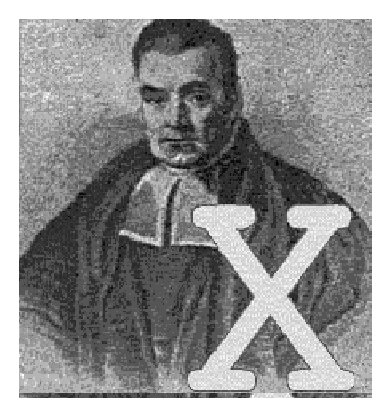
\includegraphics[scale=1.2]{grafiken/bayesicon.eps}
\end{center}
\end{figure}

\vfill

{\bf\sffamily \huge Tutorials}

\vfill

\end{center}

\begin{table}[ht]
\begin{center}
\begin{tabular}{lll}
{\em developed at} & \hspace{1.5cm} & {\em developed by} \\
University of Munich & \hspace{1.5cm} & Andreas Brezger \\
Department of Statistics & \hspace{1.5cm} & Thomas Kneib \\
Ludwigstr. 33 & \hspace{1.5cm} & Stefan Lang \\
80539 Munich & \hspace{1.5cm} & \\
  & & \\
{\em with contributions by}  &  \hspace{1.5cm} &  {\em supported by} \\
Christiane Belitz&  \hspace{1.5cm} & Ludwig Fahrmeir (mentally) \\
Eva--Maria Fronk  & \hspace{1.5cm} & Leo Held (mentally) \\
Andrea Hennerfeind & \hspace{1.5cm} & German Science Foundation  \\
Manuela Hummel & \\
Alexander Jerak & \\
Petra Kragler & \\
Leyre Osuna Echavarr\'{\i}a& \\
\end{tabular}
\end{center}
\end{table}


\newpage

\subsection*{Acknowledgements}

The development of {\em BayesX} has been supported by grants from
the German National Science Foundation (DFG),
Sonderforschungsbereich 386.

Special thanks go to (in alphabetical order of first names):

{\em Dieter Gollnow} for computing and providing the map of Munich (a really hard job); \\
{\em Leo Held} for advertising the program; \\
{\em Ludwig Fahrmeir} for his patience with finishing the program
and for carefully
reading and correcting the  manual; \\
{\em Ngianga-Bakwin Kandala} for being the first user of the program (a really hard job); \\
{\em Samson Babatunde Adebayo} for carefully reading and correcting the manual; \\
{\em Ursula Becker} for carefully reading and correcting the manual;

\subsection*{Licensing agreement} The authors of this software grant
to any individual or non-commercial organization the right to use
and to make an unlimited number of copies of this software. Usage by
commercial entities requires a license from the authors. You may not
decompile, disassemble, reverse engineer, or modify the software.
This includes, but is not limited to modifying/changing any icons,
menus, or displays associated with the software. This software
cannot be sold without written authorization from the authors. This
restriction is not intended to apply for connect time charges, or
flat rate connection/download fees for electronic bulletin board
services. The authors of this program accept no responsibility for
damages resulting from the use of this software and make no warranty
on representation, either express or implied, including but not
limited to, any implied warranty of merchantability or fitness for a
particular purpose. This software is provided as is, and you, its
user, assume all risks when using it.

\vspace{0.5cm}

{\em BayesX} is available at {
\href{http://www.stat.uni-muenchen.de/~bayesx}{http://www.stat.uni-muenchen.de/\~{}bayesx}}

\newpage

\chapter[A tutorial
on Bayesian semiparametric regression using MCMC
techniques]{Determinants of childhood undernutrition in Zambia: A
tutorial on Bayesian semiparametric regression using MCMC
techniques} \label{zambiaanalysis}

In this chapter we present a tutorial like example for the usage of
{\em bayesreg objects}. We use data on undernutrition of children in
Zambia, compare \autoref{zambia} for a description of the data set.
The files containing the data and the map can be found in the
subdirectory #examples# of the installation directory together with
the batch file #mcmctutorial.prg# containing all commands used in
the following subsections.

The rest of the example is separated in seven parts dealing with the
different steps of estimating a regression model. In
\autoref{zambia_mcmc_datasets} we create a {\em dataset object} to
incorporate, handle and manipulate the data. We will also give a
brief description of some methods that may be applied to {\em
dataset objects}. Since we want to estimate a spatial effect of the
district in which a child lives, we need the boundaries of the
districts to compute the neighborhood information of the map of
Zambia. This information will be stored in a {\em map object}.
\autoref{zambia_mcmc_maps} describes how to create and handle these
objects. Estimation of the regression model is carried out in
\autoref{zambia_mcmc_regression} using a {\em bayesreg object}. The
next two sections describe how to visualize the estimation results
and how to customize the obtained graphics.
\autoref{zambia_mcmc_postest} describes post estimation commands
which can be used to investigate the sampling paths and the
autocorrelation functions of the estimated parameters. In a last
section we perform a sensitivity analysis to assess the impact of
hyperparameter choices on our estimation results.

Please note, that all paths within the following subsections must be
changed according to the storage location of the corresponding files
on your hard disk.

\section{Reading data set
information}\label{zambia_mcmc_datasets}

In a first step we read the available data set information into {\it
BayesX}. Therefore we create a {\it dataset object} named #d#:

#> dataset d#

We store the data in #d# using the method #infile#:

#> d.infile, maxobs=5000 using c:\data\zambia.raw#

Note, that we assume the data to be provided in the external file
#c:\data\zambia.raw#. The first few lines of this file look like
this:

{\footnotesize
 hazstd bmi agc district rcw edu1 edu2 tpr sex\\
 0.0791769 \,\, 21.83 \,\, 4 \,\, 81 \,\, -1 \,\, 1 \,\, 0 \,\, 1 \,\, -1\\
 -0.2541965 \,\, 21.83 \,\, 26 \,\, 81 \,\, -1 \,\, 1 \,\, 0 \,\, 1 \,\, -1\\
 -0.1599823 \,\, 20.43 \,\, 56 \,\, 81 \,\, 1 \,\, -1 \,\, -1 \,\, 1 \,\, 1\\
 0.1733911 \,\, 22.27 \,\, 6 \,\, 81 \,\, -1 \,\, 0 \,\, 1 \,\, 1 \,\, 1}

In our example the file contains the variable names in the first
line. Therefore it is not necessary to specify them in the #infile#
command. If the file contained only the data without variable names,
we would have to supply them after the keyword #infile#:

 #> d.infile hazstd bmi agc district rcw edu1 edu2 tpr sex, maxobs=5000#
 #  using c:\data\zambia.raw#


Option #maxobs# can be used to speed up the execution time of the
#infile# command. If #maxobs# is specified, {\it BayesX} allocates
enough memory to store all the data while the total amount of
required memory is unknown in advance if #maxobs# remains
unspecified. For larger data sets this may cause {\it BayesX} to
start reading the data set information several times because the
currently allocated memory is exceeded. However, this is only
meaningful for larger data sets with more than 10000 observations
and could therefore be omitted in our example.

A second option that may be added to the #infile# command is the
#missing# option to indicate missing values. Specifying for example
{\tt missing=M} defines the letter '{\tt M}' as an indicator for a
missing value. The default for missing values are a period '.' and
'{\tt NA}' (which remain valid indicators for missing values even if
an additional indicator is defined by the {\tt missing} option).

After having read in the data set information we can inspect the
data visually. Executing the command

#> d.describe#

opens an {\it object-viewer window} containing the data in form of a
spreadsheet. This can also be achieved by double-clicking on the
{\it dataset object} in the {\it object browser}.

Further methods allow to examine the variables in the {\it dataset
object}. For a categorial variable, e.g.~#sex#, the #tabulate#
command may be used to produce a frequency table:

#> d.tabulate sex#

resulting in

\begin{verbatim}
Variable: sex

          Value       Obs           Freq            Cum
             -1      2451         0.5057         0.5057
              1      2396         0.4943              1
\end{verbatim}

being printed in the {\it output window}. For continuous variables
the #descriptive# command prints several characteristics of the
variable in the {\em output window}. E.g., executing

#> d.descriptive bmi#

leads to

\begin{verbatim}
   Variable    Obs        Mean      Median         Std         Min         Max
        bmi   4847   21.944349        21.4   3.2879659        12.8       39.29
\end{verbatim}

\section{Map objects}\label{zambia_mcmc_maps}

In the following we want to estimate a spatially correlated effect
of the district in which a child lives. Therefore we need the
boundaries of the districts in Zambia to compute the neighborhood
information of the map of Zambia. We therefore create a {\it map
object}

#> map m#

and read in the boundaries using the #infile# command of {\it map
objects}:

#> m.infile using c:\data\zambia.bnd#

Having read in the boundary information, {\it BayesX} automatically
computes the neighborhood matrix of the map.

The file following the keyword #using# is assumed to contain the
boundaries in form of closed polygons. Compare chapter \ref*{map} of
the reference manual for a description of the expected file format.

{\it Map objects} may be visualized using method #describe#:

#> m.describe#

resulting in the graph shown in \autoref{zambia_mcmc_zambiamap}.
Additionally, #describe# prints further information about the {\it
map object} in the {\it output window} including the name of the
object, the number of regions, the minimum and maximum number of
neighbors and the bandwidth of the corresponding adjacency or
neighborhood matrix:

\begin{verbatim}
  MAP m
  Number of regions: 54
  Minimum number of neighbors: 1
  Maximum number of neighbors: 9
  Bandsize of corresponding adjacency matrix: 24
\end{verbatim}

\begin{figure}[ht]
\begin{center}
\epsfig{file=grafiken/zambia.ps,scale=0.35} {\it\caption{The
districts within Zambia.\label{zambia_mcmc_zambiamap}}}
\end{center}
\end{figure}


The numerical complexity associated with the estimation of
structured spatial effects using MCMC techniques depends essentially
on the structure of the neighborhood matrix. Often the geographical
information stored in a boundary file does not represent the 'ideal'
ordering (as regards to the estimation problem) of the districts or
regions. Therefore it may be useful to reorder the map using method
#reorder#:

#> m.reorder#

Usually reordering results in a smaller bandwidth although the
bandwidth is not the criterion that is minimized by #reorder#.
Instead the {\it envelope} of the neighborhood matrix is minimized
(compare George and Liu 1981).

In order to avoid reordering the {\it map object} every time you
start {\it BayesX} it is useful to store the reordered version in a
separate file. This can be achieved using the #outfile# command of
{\it map objects}:

#> m.outfile, replace using c:\data\zambiasort.bnd#

The reordered map is now stored in the given file. Note, that
specifying the option #replace# allows {\it BayesX} to overwrite an
existing file with the same name. Without this option an error
message would be raised if the given file is already existing.

Reading the boundary information from an external file and computing
the neighborhood matrix may be a computationally intensive task if
the map contains a large number of regions or if the polygons are
given in great detail. To avoid doing these computation in every
$BayesX$ session, we store the neighborhood information in a
so-called {\it graph file} using method #outfile# together with the
#graph# option (compare chapter \ref*{map} of the reference manual
for a description of {\em graph files}):

#> m.outfile, replace graph using c:\data\zambiasort.gra#

To see how storing maps in {\it graph files} affects the computation
time of the #infile# command, we create a second {\it map object}
and read in the information from the graph file. Again, we have to
specify the keyword #graph#:

#> map m1#\\
#> m1.infile, graph using c:\data\zambiasort.gra#

As you should have noticed, reading geographical information from a
{\it graph file} is usually much faster than reading from a {\it
boundary file}. However, using {\it graph files} also has a
drawback. Since they do no longer contain the full information on
the polygons forming the map, we can not visualize a {\it map
object} created from a {\it graph file}. Trying to do so

#> m1.describe#

raises an error message. This implies, that visualizing estimation
results of spatial effects can only be based on {\it map objects}
created from {\it boundary files}, although estimation can be
carried out using {\it graph files}. Since we will work with the
{\it map object} #m# in the following, we delete #m1#:

#> drop m1#

\section{Bayesian semiparametric
regression}\label{zambia_mcmc_regression}

To estimate a regression model using MCMC techniques we first create
a {\it bayesreg object}:

#> bayesreg b#

By default estimation results are written to the subdirectory
#output# of the installation directory. In this case the default
filenames are composed of the name of the {\it bayesreg object} and
the type of the specific file. Usually it is more convenient to
store the results in a user-specified directory. To define this
directory we use the #outfile# command of {\it bayesreg objects}:

#> b.outfile = c:\data\b#

Note, that #outfile# does not only specify a directory but also a
base filename (the character #b# in our example). Therefore
executing the command above leads to storage of the results in the
directory #c:\data# and all filenames start with the character #b#.
Of course the base filename may be different from the name of the
{\it bayesreg object}.

In addition to parameter estimates {\it BayesX} also gives
acceptance rates for the different effects and some further
information on the estimation process. In contrast to parameter
estimates this information is not stored automatically but is
printed in the {\it output window}. Therefore it is useful to store
the contents of the {\it output window}. This can be achieved
automatically by opening a log file using the #logopen# command

#> logopen, replace using c:\data\logmcmc.txt#

After opening a log file, every information written to the {\em
output window} is also stored in the log file. Option #replace#
allows {\it BayesX} to overwrite an existing file with the same name
as the specified log file. Without #replace# results are appended to
an existing file.

The model presented in Kandala et al.~(2001) is given by the
following semiparametric predictor:
\[\eta=\gamma_0+\gamma_1rcw+\gamma_2edu1+\gamma_3edu2+\gamma_4tpr+\gamma_5sex+f_1(bmi)+f_2(agc)+f^{str}(district)+f^{unstr}(district)\]
The two continuous covariates #bmi# and #agc# are assumed to have a
possibly nonlinear effect on the Z-score and are therefore modelled
nonparametrically (as P-splines with second order random walk prior
in our example). The spatial effect of the district is split up into
a spatially correlated part $ f^{str}(district)$ and an uncorrelated
part $f^{unstr}(district)$, see Fahrmeir and Lang (2001b) for a
motivation. The correlated part is modelled by a Markov random field
prior, where the neighborhood matrix and possible weights associated
with the neighbors are obtained from the {\it map object} #m#. The
uncorrelated part is modelled by an i.i.d.~Gaussian effect.

To estimate the model we use method #regress# of {\em bayesreg
objects}:

 #> b.regress hazstd = rcw + edu1 + edu2 + tpr + sex + bmi(psplinerw2)#\\
 #  + agc(psplinerw2) + district(spatial,map=m) + district(random),#\\
 #  family=gaussian iterations=12000 burnin=2000 step=10 predict using d#

Options {\tt iterations}, {\tt burnin} and {\tt step} define
properties of the MCMC-algorithm. The total number of MCMC
iterations is given by {\tt iterations} while the number of burn in
iterations is given by {\tt burnin}. Therefore we obtain a sample of
10000 random numbers with the above specifications. Since, in
general, these random numbers are correlated, we do not use all of
them but thin out the Markov chain by the thinning parameter {\tt
step}. Specifying {\tt step=10} as above forces {\em BayesX} to
store only every 10th sampled parameter which leads to a random
sample of length 1000 for every parameter in our example.

Note, that the choice of {\tt iterations} also affects computation
time. On a 2.4 GHz PC estimation of our model took about 1 minute
and 5 seconds, which is rather fast in regard of the complexity of
the model.

If option {\tt predict} is specified, samples of the deviance, the
effective number of parameters $p_D$, and the deviance information
criteria $DIC$ of the model are computed, see Spiegelhalter et
al.~(2002). In addition, estimates for the linear predictor and the
expectation of every observation are obtained.

In the following we reproduce the content of the {\em output window}
to make the user familiar with the estimation results produced by
{\em BayesX}:

\footnotesize
\begin{verbatim}
ESTIMATION RESULTS:

  Predicted values:

  Estimated mean of predictors, expectation of response and
  individual deviances are stored in file
  c:\data\b_predictmean.raw

  Estimation results for the deviance:

  Unstandardized Deviance (-2*Loglikelihood(y|mu))

  Mean:             12688.959
  Std. Dev:         12.615837
  2.5% Quantile:    12663.847
  10% Quantile:     12673.03
  50% Quantile:     12688.804
  90% Quantile:     12705.921
  97.5% Quantile:   12714.078

  Saturated Deviance (-2*Loglikelihood(y|mu) + 2*Loglikelihood(y|mu=y))

  Mean:             4848.1335
  Std. Dev:         98.563486
  2.5% Quantile:    4657.7394
  10% Quantile:     4719.1869
  50% Quantile:     4847.534
  90% Quantile:     4971.7679
  97.5% Quantile:   5059.5874

  Samples of the deviance are stored in file
  c:\data\b_deviance_sample.raw

  Estimation results for the DIC:

  DIC based on the unstandardized deviance

  Deviance(bar_mu):           12639.654
  pD:                         49.305405
  DIC:                        12738.265


  DIC based on the saturated deviance

  Deviance(bar_mu):           4797.8139
  pD:                         50.31962
  DIC:                        4898.4532

  Estimation results for the scale parameter:

  Acceptance rate:   100 %

  Mean:             0.802517
  Std. dev.:        0.0164098
  2.5% Quantile:    0.768981
  10% Quantile:     0.782025
  50% Quantile:     0.802168
  90% Quantile:     0.824066
  97.5% Quantile:   0.83595


  FixedEffects1

  Acceptance rate:    100 %

  Variable  mean           Std. Dev.      2.5% quant.    median         97.5% quant.
  const     0.102975       0.0493194      0.00460694     0.102048       0.201918
  rcw       0.00782474     0.0129786      -0.0177587     0.0079339      0.0325389
  edu1      -0.0612525     0.0268997      -0.11368       -0.0622293     -0.00870588
  edu2      0.234627       0.0468064      0.146532       0.23578        0.322222
  tpr       0.0891162      0.0218746      0.0476786      0.0893937      0.133562
  sex       -0.058801      0.0130027      -0.083714      -0.0593365     -0.031744

  Results for fixed effects are also stored in file
  c:\data\b_FixedEffects1.res


  f_bmi_pspline

  Acceptance rate:    100 %

  Results are stored in file
  c:\data\b_f_bmi_pspline.res

  Postscript file is stored in file
  c:\data\b_f_bmi_pspline.ps

  Results may be visualized using method 'plotnonp'
  Type for example: objectname.plotnonp 1


  f_bmi_pspline_variance

  Acceptance rate:    100 %

  Estimation results for the variance component:

  Mean:             0.00192786
  Std. dev.:        0.00268103
  2.5% Quantile:    0.000281651
  10% Quantile:     0.000452872
  50% Quantile:     0.00119819
  90% Quantile:     0.00380296
  97.5% Quantile:   0.00806144

  Results for the variance component are also stored in file
  c:\data\b_f_bmi_pspline_var.res


  f_agc_pspline

  Acceptance rate:    100 %

  Results are stored in file
  c:\data\b_f_agc_pspline.res

  Postscript file is stored in file
  c:\data\b_f_agc_pspline.ps

  Results may be visualized using method 'plotnonp'
  Type for example: objectname.plotnonp 3


  f_agc_pspline_variance

  Acceptance rate:    100 %

  Estimation results for the variance component:

  Mean:             0.00600587
  Std. dev.:        0.00993897
  2.5% Quantile:    0.00119369
  10% Quantile:     0.00169024
  50% Quantile:     0.00397818
  90% Quantile:     0.0107538
  97.5% Quantile:   0.0227737

  Results for the variance component are also stored in file
  c:\data\b_f_agc_pspline_var.res


  f_district_spatial

  Acceptance rate:    100 %

  Results are stored in file
  c:\data\b_f_district_spatial.res

  Postscript file is stored in file
  c:\data\b_f_district_spatial.ps

  Results may be visualized in BayesX using method 'drawmap'
  Type for example: objectname.drawmap 5


  f_district_spatial_variance

  Acceptance rate:    100 %

  Estimation results for the variance component:

  Mean:             0.0359038
  Std. dev.:        0.0176849
  2.5% Quantile:    0.0117425
  10% Quantile:     0.0168868
  50% Quantile:     0.0321435
  90% Quantile:     0.0593765
  97.5% Quantile:   0.0807406

  Results for the variance component are also stored in file
  c:\data\b_f_district_spatial_var.res


  f_district_random

  Acceptance rate:    100 %

  Results for random effects are stored in file
  c:\data\b_f_district_random.res

  Results for the sum of the structured and unstructured
  spatial effects are stored in file
  c:\data\b_district_spatialtotal.res


  f_district_random_variance

  Acceptance rate:    100 %

  Estimation results for the variance component:

  Mean:             0.0077143
  Std. dev.:        0.00580379
  2.5% Quantile:    0.000703806
  10% Quantile:     0.00152536
  50% Quantile:     0.00648848
  90% Quantile:     0.0153428
  97.5% Quantile:   0.0215434

  Results for the variance component are also stored in file
  c:\data\b_f_district_random_var.res

  Files of model summary:

  ---------------------------------------------------------------------------

  Batch file for visualizing effects of nonlinear functions is stored in file
  c:\data\b_graphics.prg

  NOTE: 'input filename' must be substituted by the filename of the boundary-file

  ---------------------------------------------------------------------------

  Batch file for visualizing effects of nonlinear functions
  in S-Plus is stored in file
  c:\data\b_splus.txt

  NOTE: 'input filename' must be substituted by the filename of the boundary-file

  ---------------------------------------------------------------------------

  Latex file of model summaries is stored in file
  c:\data\b_model_summary.tex

  ---------------------------------------------------------------------------
\end{verbatim}
\normalsize

In addition to the information being printed to the {\em output
window} results for each effect are written to external ASCII files.
The names of these files are given in the {\em output window},
compare the previous pages. The files contain the posterior mean and
median, the posterior 2.5\%, 10\%, 90\% and 97.5\% quantiles, and
the corresponding 95\% and 80\% posterior probabilities of the
estimated effects. For example, the beginning of the file
#c:\data\b_f_bmi_pspline.res# for the effect of # bmi# looks like
this:

{\footnotesize
 intnr \,\, bmi \,\, pmean \,\, pqu2p5 \,\, pqu10 \,\, pmed \,\, pqu90 \,\, pqu97p5 \,\, pcat95 \,\, pcat80\\
 1 \,\, 12.8 \,\, -0.284065 \,\, -0.660801 \,\, -0.51678 \,\, -0.283909 \,\, -0.0585753 \,\, 0.085998 \,\, 0 \,\, -1\\
 2 \,\, 13.15 \,\, -0.276772 \,\, -0.609989 \,\, -0.483848 \,\, -0.275156 \,\, -0.070517 \,\, 0.0572406 \,\, 0 \,\, -1\\
 3 \,\, 14.01 \,\, -0.258674 \,\, -0.515628 \,\, -0.416837 \,\, -0.257793 \,\, -0.10009 \,\, -0.00289024 \,\, -1 \,\, -1}

The posterior quantiles and posterior probabilities may be changed
by the user using the options #level1# and #level2#. For example
specifying #level1=99# and #level2=70# in the options list of the
#regress# command leads to the computation of 0.5\%, 15\%, 85\% and
99.5\% quantiles of the posterior. The defaults are #level1=95# and
#level2=80#.

Some nonparametric effects are visualized by {\em BayesX}
automatically and the resulting graphs are stored in ps format.
E.g.~the effect of #bmi# is visualized in the file
#c:\data\b_f_bmi_pspline.ps# (compare the results on the previous
pages for the other filenames). In addition to the postscript files
a file containing the commands to reproduce the graphics is stored
in the output directory. In our example the name of the file is
#c:\data\b_graphics.prg#. The advantage is that additional options
may be added by the user to customize the graphs (compare the
following two subsubsections).

Moreover a file with ending #.tex# is created in the outfile
directory. This file contains a summary of the estimation results
and may be compiled using \LaTeX.

Having finished the estimation we may close the log file by typing

#> logclose#

Note, that the log file is closed automatically when you exit {\em
BayesX}.

\section{Visualizing estimation results}\label{zambia_mcmc_visual}

{\em BayesX} provides three possibilities to visualize estimation
results:
\begin{itemize}
\item As mentioned in the previous subsubsection, certain results
are automatically visualized by {\em BayesX} and stored in
postscript files. \item Post estimation commands of {\em bayesreg
objects} allow to visualize results after having executed a
#regress# command. \item {\em Graph objects} may be used to produce
graphics using the ASCII files containing the estimation results. In
principle {\em graph objects} allow the visualization of any content
of a {\em dataset object}. {\em Graph files} are also used in the
batch file containing the commands to reproduce the automatically
generated graphics.
\end{itemize}

In this subsubsection we describe the general usage of the post
estimation commands as well as the commands for the usage with {\em
graph objects} to enable the user to reproduce the automatically
generated plots directly in {\em BayesX}.
\autoref{zambia_mcmc_custom} describes how to customize plots.

\subsection{Post estimation commands}

After having estimated a regression model plots for nonparametric
effects of continuous covariates can be produced using the post
estimation command #plotnonp#:

#> b.plotnonp 1#

and

#> b.plotnonp 3#

produce the graphs shown in \autoref{zambia_mcmc_bmi1} in an {\it
object-viewer window}. The numbers following the #plotnonp# command
depend on the order in which the model terms have been specified.
The numbers are supplied in the {\em output window} after
estimation, compare the results in the previous subsubsection.

By default the plots contain the posterior mean and pointwise
credible intervals according to the levels specified in the
#regress# command. So by default the plot includes pointwise 80\%
and 95\% credible intervals.

\begin{figure}[ht]
\begin{center}
\epsfig{file=grafiken/zambia_mcmc_f_bmi1.ps,scale=0.5}
\epsfig{file=grafiken/zambia_mcmc_f_age1.ps,scale=0.5}
{\it\caption{Effect of the body mass index of the child`s mother and
of the age of the child together with pointwise 80\% and 95\%
credible intervals. \label{zambia_mcmc_bmi1}}}
\end{center}
\end{figure}

A plot may be stored in ps format using the #outfile# option.
Executing

#> b.plotnonp 1, replace outfile = c:\data\f_bmi.ps#

stores the plot for the estimated effect of #bmi# in the file
#c:\data\f_bmi.ps#. Again, specifying #replace# allows {\it BayesX}
to overwrite an existing file. Note, that {\it BayesX} does not
display the graph on the screen if the option #outfile# is
specified.

Estimation results for spatial effects are best visualized by
drawing the respective map and coloring the regions of the map
according to some characteristic of the posterior, e.g.~the
posterior mean. For the structured spatial effect this can be
achieved using the post estimation command #drawmap#

#> b.drawmap 5#

which results in the graph shown in \autoref{zambia_mcmc_spat1}.

\begin{figure}[ht]
\begin{center}
\epsfig{file=grafiken/zambia_mcmc_f_spat1.ps,scale=0.35}
{\it\caption{Posterior mean of the structured spatial
effect.\label{zambia_mcmc_spat1}}}
\end{center}
\end{figure}

\subsection{Graph Objects}

The commands presented in the previous paragraph work only after
having estimated a regression model in the current {\em BayesX}
session but it may also be useful to visualize results of former
analyses. This can be achieved using {\em graph objects}. Note
again, that {\em graph files} are also used in the batch file
containing the commands to reproduce the automatically generated
graphics. Therefore the purpose of this paragraph is also to enable
the user to understand the content of this batch file.

First we read the estimation results into a {\it dataset object}.
For example the estimation results for the effect of #bmi# can be
read into {\it BayesX} by executing the commands

#> dataset res#\\
#> res.infile using c:\data\b_f_bmi_pspline.res#

Now the estimation results (or any content of a {\it dataset
object}) may be visualized using a {\it graph object} which we
create by typing

#> graph g#

The results stored in the {\em dataset object} #res# are now
visualized using the #plot# command of {\it graph objects}.
Executing

#> g.plot bmi pmean pqu2p5 pqu10 pqu90 pqu97p5 using res#

reproduces the graph in \autoref{zambia_mcmc_bmi1}.

Similar as for #plotnonp#, the direct usage of the #drawmap# command
is only possible after executing a #regress# command. However, using
{\it graph objects} again allows us to visualize results that have
been stored in a file.

First we read the information contained in this file into a {\it
dataset object}. For example the following command

#> res.infile using c:\data\b_f_district_spatial.res#

stores the estimation results for the structured spatial effect in
the {\em dataset object} #res#. Now we can visualize the posterior
mean using method #drawmap# of {\it graph objects} leading again to
the graph shown in \autoref{zambia_mcmc_spat1}:

#> g.drawmap pmean district, map=m using res#

Since -- in contrast to a {\it bayesreg object} -- no {\it map
object} is associated with a {\it graph object} we have to specify
the map that we want to use explicitly in the options list.

Using {\it graph objects} also allows us to plot other
characteristics of the posterior than the posterior mean. For
instance the posterior 95\% probabilities may be visualized by

#> g.drawmap pcat95 district, map=m using res#

The result is shown in \autoref{zambia_mcmc_spat2}.

\begin{figure}[ht]
\begin{center}
\epsfig{file=grafiken/zambia_mcmc_f_spat2.ps,scale=0.35}
{\it\caption{Posterior 95\% probability of the structured spatial
effect.\label{zambia_mcmc_spat2}}}
\end{center}
\end{figure}

A further advantage of {\it graph objects} is, that they allow to
visualize the estimation results for the uncorrelated spatial
effects. Since these are modelled as unstructured random effects,
{\it BayesX} is unable to recognize them as spatial effects.
However, proceeding as follows gives us the possibility to plot the
unstructured spatial effect shown in \autoref{zambia_mcmc_random1}:

#> res.infile using c:\data\b_f_district_random.res#\\
#> g.drawmap pmean district, map=m using res#

\begin{figure}[ht]
\begin{center}
\epsfig{file=grafiken/zambia_mcmc_f_random1.ps,scale=0.35}
{\it\caption{Posterior mean of the unstructured spatial
effect.\label{zambia_mcmc_random1}}}
\end{center}
\end{figure}

\section{Customizing graphics}\label{zambia_mcmc_custom}

This subsubsection describes how to customize graphics created in
{\em BayesX}. All options are described for the usage with the post
estimation commands but may be used with graph files as well. So the
options presented in this subsubsection also enable the user to
modify the batch file containing the commands to reproduce the
automatically generated graphics.

For the presentation of nonparametric effects it may be desirable to
include only one of the credible intervals into the plot. This is
achieved by specifying the #levels# option. Possible values of this
option are #1# and #2#, corresponding to the levels specified in the
#regress# command (compare \autoref{zambia_mcmc_regression}). If the
default values of #level1# and #level2# have been used, specifying
#levels=2# in the #plotnonp# command causes {\it BayesX} to plot the
80\% credible interval only (\autoref{zambia_mcmc_bmi3}):

#> b.plotnonp 1, levels=2#

\begin{figure}[ht]
\begin{center}
\epsfig{file=grafiken/zambia_mcmc_f_bmi3.ps,scale=0.5}
{\it\caption{Effect of the body mass index of the child`s mother
with pointwise 80\% credible interval
only.\label{zambia_mcmc_bmi3}}}
\end{center}
\end{figure}

It may be useful to add some more information to the graphs of
nonparametric effects to distinguish more obviously between
different covariates. Ways to do so are the specification of a title
or the specification of axis labels. Both possibilities are
supported by {\it BayesX} as demonstrated in the following examples
(compare \autoref{zambia_mcmc_bmi4} for the resulting plots):

 #> b.plotnonp 1, title="Mother body mass index"#\\
 #> b.plotnonp 1, xlab="bmi" ylab="f_bmi" title="Mother body mass index"#

\begin{figure}[ht]
\begin{center}
\begin{multicols}{2}
\epsfig{file=grafiken/zambia_mcmc_f_bmi4.ps,scale=0.5}
\epsfig{file=grafiken/zambia_mcmc_f_bmi5.ps,scale=0.5}
\end{multicols}
{\it\caption{Specification of title and axis
labels.\label{zambia_mcmc_bmi4}}}
\end{center}
\end{figure}

By default {\it BayesX} displays x- and y-axis with five equidistant
ticks according to the range of the data that is to be visualized.
These defaults may be overwritten using the options #xlimbottom#,
#xlimtop# and #xstep# for the x-axis and #ylimbottom#, #ylimtop# and
#ystep# for the y-axis, respectively. The usage of these options is
more or less self-explanatory and is demonstrated in the following
commands which lead to the graph shown in
\autoref{zambia_mcmc_bmi6}.

#> r.plotnonp 1, xlab="bmi" ylab="f_bmi" title="Mother body mass index"#\\
#  ylimbottom=-0.8 ylimtop=0.6 ystep=0.2 xlimbottom=12 xlimtop=40#

\autoref{zambia_mcmc_bmi6} also includes a graph for the effect of
the age of the child that is customized in the same way as for the
effect of #bmi#.

#> r.plotnonp 3, xlab="age" ylab="f_age" title="Age of the child in months"#\\
#  ylimbottom=-0.3  ystep=0.3 xlimbottom=0 xlimtop=60 xstep=10#

\begin{figure}[ht]
\begin{center}
\epsfig{file=grafiken/zambia_mcmc_f_bmi6.ps,scale=0.5}
\epsfig{file=grafiken/zambia_mcmc_f_age2.ps,scale=0.5}
{\it\caption{Re-defining x- and y-axis.\label{zambia_mcmc_bmi6}}}
\end{center}
\end{figure}

Now we turn to the options for method #drawmap#. By default
#drawmap# uses grey scales to represent different values of the
posterior mean. Using the option #color# forces {\it BayesX} to use
different colors instead. Here the default would be to represent
higher values through green colors and smaller values through red
colors. Specifying #swapcolors# switches this definition. Therefore
the following command

#> b.drawmap 5, color swapcolors#

leads to the graph shown in \autoref{zambia_mcmc_spat3} with higher
values being represented through red colors and smaller values
through green colors.

\begin{figure}[ht]
\begin{center}
\epsfig{file=grafiken/zambia_mcmc_f_spat3.ps,scale=0.35}
{\it\caption{Posterior mean of the structured spatial effect in
color.\label{zambia_mcmc_spat3}}}
\end{center}
\end{figure}

Similar options as for the visualization of nonparametric effects
exist for method #drawmap#. For example, a title may be included by
specifying the option #title#

#> b.drawmap 5, color swapcolors title="Structured spatial effect"#

or the range of values to be displayed may be defined using the
options #lowerlimit# and #upperlimit#:

#> b.drawmap 5, color swapcolors title="Structured spatial effect" lowerlimit=-0.3#\\
#  upperlimit=0.3#

The graph produced by the second command is shown in
\autoref{zambia_mcmc_spat4}.

\begin{figure}[ht]
\begin{center}
\epsfig{file=grafiken/zambia_mcmc_f_spat4.ps,scale=0.35}
{\it\caption{Specifying a title and the range of the plot for
spatial effects.\label{zambia_mcmc_spat4}}}
\end{center}
\end{figure}

\section{Autocorrelation functions and sampling
paths}\label{zambia_mcmc_postest}

{\em Bayesreg objects} provide some post estimation commands to get
sampled parameters or to plot autocorrelation functions of sampled
parameters. For example

#> b.plotautocor, maxlag=250#

computes and displays the autocorrelation functions for all
estimated parameters with #maxlag# specifying the maximum lag number
(\autoref{zambia_mcmc_autocor1} shows a small part of the resulting
graph).

If the number of parameters is large this may be computationally
expensive, so {\it BayesX} provides a second possibility to compute
autocorrelation functions. Adding the option #mean# to the
#plotautocor# command as in

\begin{figure}[ht]
\begin{center}
\epsfig{file=grafiken/zambia_mcmc_autocor1.eps,scale=0.75}
{\it\caption{Autocorrelation function for the scale parameter and
the intercept.\label{zambia_mcmc_autocor1}}}
\end{center}
\end{figure}

#> b.plotautocor, mean#

leads to the computation of only the minimum, mean and maximum
autocorrelation functions. The result for the scale parameter is
shown in \autoref{zambia_mcmc_autocor2}.

\begin{figure}[ht]
\begin{center}
\epsfig{file=grafiken/zambia_mcmc_autocormean1.ps,scale=0.5}
{\it\caption{Minimum, mean and maximum autocorrelation function for
the scale parameter.\label{zambia_mcmc_autocor2}}}
\end{center}
\end{figure}

Note, that executing the #plotautocor# command also stores the
computed autocorrelation functions in a file named #autocor.raw# in
the output directory of the {\it bayesreg object}.

To save memory, the sampling paths of the estimated parameters are
only stored temporarily by default and will be destroyed, when the
corresponding {\em bayesreg object} is deleted. If we want to store
the sampling paths permanently, we have to execute the #getsample#
command

#> b.getsample#

which stores the sampled parameters in ASCII files in the output
directory. To avoid too large files, the samples are typically
partitioned into several files. Executing the #getsample# command
also produces postscript files of the sampling paths in the output
directory (compare \autoref{zambia_mcmc_sample1} for the content of
one of these files).

\begin{figure}[ht]
\begin{center}
\epsfig{file=grafiken/zambia_mcmc_intercept_sample.eps,scale=0.75}
{\it\caption{Sampling path of the
intercept.\label{zambia_mcmc_sample1}}}
\end{center}
\end{figure}

\section{Sensitivity analysis}\label{zambia_mcmc_sensitivity}

In some situations the estimation results of a full Bayesian
semiparametric regression model depend on the choice of
hyperparameters, e.g.~the parameters #a# and #b# defining the
inverse gamma prior of the variances of nonparametric and spatial
effects. It is often recommended to check how sensitive the results
are with respect to changes in the hyperparameters. In the following
we will re-estimate the model from \autoref{zambia_mcmc_regression}
with different choices for the hyperparameters #a# and #b# for each
effect in the model. The standard choices for #a# and #b# are
#a=b=0.001#. As a first trial we choose a smaller value for #a# and
#b#:

#> b.regress hazstd = rcw + edu1 + edu2 + tpr + sex#\\
#  + bmi(psplinerw2,a=0.00001,b=0.00001) + agc(psplinerw2,a=0.00001,b=0.00001)#\\
#  + district(spatial,map=m,a=0.00001,b=0.00001)#\\
#  + district(random,a=0.00001,b=0.00001), family=gaussian iterations=12000#\\
#  burnin=2000 step=10 predict using d#


\autoref{zambia_mcmc_sensi1} shows the results for the nonparametric
effects with this choice of hyperparameters. Obviously, the
estimated functions are somewhat smoother but they do not differ
that much from the estimates with the standard choices.

\begin{figure}[ht]
\begin{center}
\epsfig{file=grafiken/zambia_mcmc_f_bmi7.ps,scale=0.5}
\epsfig{file=grafiken/zambia_mcmc_f_age3.ps,scale=0.5}
{\it\caption{Results for the nonparametric effects with
hyperparameters {\em\tt a=b=0.00001} for nonparametric and spatial
effects.\label{zambia_mcmc_sensi1}}}
\end{center}
\end{figure}

Now we try two further choices for the hyperparameters, with both
#a=1# and #b# small. We estimate models with #b=0.005# and
#b=0.00005#:

#> b.regress hazstd = rcw + edu1 + edu2 + tpr + sex + bmi(psplinerw2,a=1,b=0.005)#\\
#  + agc(psplinerw2,a=1,b=0.005) + district(spatial,map=m,a=1,b=0.005)#\\
#  + district(random,a=1,b=0.005), family=gaussian iterations=12000 burnin=2000#\\
#  step=10 predict using d#

#> b.regress hazstd = rcw + edu1 + edu2 + tpr + sex + bmi(psplinerw2,a=1,b=0.00005)#\\
#  + agc(psplinerw2,a=1,b=0.00005) + district(spatial,map=m,a=1,b=0.00005)#\\
#  + district(random,a=1,b=0.00005), family=gaussian iterations=12000 burnin=2000#\\
#  step=10 predict using d#

\autoref{zambia_mcmc_sensi2} and \autoref{zambia_mcmc_sensi3}
contain the results for the nonparametric effects for the two
choices of hyperparameters.

\begin{figure}[ht]
\begin{center}
\epsfig{file=grafiken/zambia_mcmc_f_bmi8.ps,scale=0.5}
\epsfig{file=grafiken/zambia_mcmc_f_age4.ps,scale=0.5}
{\it\caption{Results for the nonparametric effects with hyper
parameters {\em\tt a=1} and {\em\tt b=0.005} for nonparametric and
spatial effects.\label{zambia_mcmc_sensi2}}}
\end{center}
\end{figure}

\begin{figure}[ht]
\begin{center}
\epsfig{file=grafiken/zambia_mcmc_f_bmi9.ps,scale=0.5}
\epsfig{file=grafiken/zambia_mcmc_f_age5.ps,scale=0.5}
{\it\caption{Results for the nonparametric effects with hyper
parameters {\em\tt a=1} and {\em\tt b=0.00005} for nonparametric and
spatial effects.\label{zambia_mcmc_sensi3}}}
\end{center}
\end{figure}

\chapter[A tutorial
on Bayesian semiparametric regression using GLMM
methodology]{Determinants of childhood undernutrition in Zambia: A
tutorial on Bayesian semiparametric regression using GLMM
methodology} \label{remlregzambiaanalysis}

To make the user familiar with the usage of {\em remlreg objects} we
present a tutorial like example in this subsection. We use data on
undernutrition of children in Zambia, compare \autoref{zambia} for a
description of the data set. The files containing the data and the
map can be found in the subdirectory #examples# of the installation
directory together with the batch file #remltutorial.prg# containing
all commands used in the following subsections.

The rest of the example is organized as follows: In
\autoref{zambia_reml_datasets} we create a {\em dataset object} to
incorporate, handle and manipulate the data. We will also give a
brief description of some methods that may be applied to {\em
dataset objects}. Since we want to estimate a spatial effect of the
district in which a child lives, we need the boundaries of the
districts to compute the neighborhood information of the map of
Zambia. This information will be stored in a {\em map object}.
\autoref{zambia_reml_maps} describes how to create and handle these
objects. Estimation of the regression model is carried out in
\autoref{zambia_reml_regression} using a {\em remlreg object}. The
last two subsubsections describe how to visualize the estimation
results and how to customize the obtained graphics.

Please note, that all paths within the following subsections must be
changed according to the storage location of the corresponding files
on your hard disk.

\section{Reading data set information}\label{zambia_reml_datasets}

In a first step we read the available data set information into {\it
BayesX}. Therefore we create a {\it dataset object} named #d#:

#> dataset d#

We store the data in #d# using the method #infile#:

#> d.infile, maxobs=5000 using c:\data\zambia.raw#

Note, that we assume the data to be provided in the external file
#c:\data\zambia.raw#. The first few lines of this file look like
this:

{\footnotesize
 hazstd bmi agc district rcw edu1 edu2 tpr sex\\
 0.0791769 \,\, 21.83 \,\, 4 \,\, 81 \,\, -1 \,\, 1 \,\, 0 \,\, 1 \,\, -1\\
 -0.2541965 \,\, 21.83 \,\, 26 \,\, 81 \,\, -1 \,\, 1 \,\, 0 \,\, 1 \,\, -1\\
 -0.1599823 \,\, 20.43 \,\, 56 \,\, 81 \,\, 1 \,\, -1 \,\, -1 \,\, 1 \,\, 1\\
 0.1733911 \,\, 22.27 \,\, 6 \,\, 81 \,\, -1 \,\, 0 \,\, 1 \,\, 1 \,\, 1}

In our example the file contains the variable names in the first
line. Therefore  it is not necessary to specify them in the #infile#
command. If the file contained only the data without variable names,
we would have to supply them after the keyword #infile#:

 #> d.infile hazstd bmi agc district rcw edu1 edu2 tpr sex, maxobs=5000#\\
 #  using c:\data\zambia.raw#


Option #maxobs# can be used to speed up the execution time of the
#infile# command. If #maxobs# is specified, {\it BayesX} allocates
enough memory to store all the data while the total amount of
required memory is unknown in advance if #maxobs# remains
unspecified. For larger data sets this may cause {\it BayesX} to
start reading the data set information several times because the
currently allocated memory is exceeded. However, this is only
meaningful for larger data sets with more than 10,000 observations
and could therefore be omitted in our example.

A second option that may added to the {\tt infile} command is the
{\tt missing} option to indicate missing values. Specifying for
example {\tt missing = M} defines the letter 'M' as an indicator for
a missing value. The default for missing values are a period '.' and
'NA' (which remain valid indicators for missing values even if an
additional indicator is defined by the {\tt missing} option).

After having read in the data set information we can inspect the
data visually. Executing the command

#> d.describe#

opens an {\it Object-Viewer} window containing the data in form of a
spreadsheet. This can also be achieved by double-clicking on the
{\it dataset object} in the {\it object browser}.

Further methods allow to examine the variables in the {\it dataset
object}. For a categorial variable, e.g.~#sex#, the #tabulate#
command may be used to produce a frequency table:

#> d.tabulate sex#

resulting in

\begin{verbatim}
Variable: sex

          Value       Obs           Freq            Cum
             -1      2451         0.5057         0.5057
              1      2396         0.4943              1
\end{verbatim}

being printed in the {\it output window}. For continuous variables
the #descriptive# command prints several characteristics of the
variable in the {\em output window}. E.g., executing

#> d.descriptive bmi#

leads to

\begin{verbatim}
   Variable    Obs        Mean      Median         Std         Min         Max
        bmi   4847   21.944349        21.4   3.2879659        12.8       39.29
\end{verbatim}

\section{Map objects}\label{zambia_reml_maps}

In the following we want to estimate a spatially correlated effect
of the district in which a child lives. Therefore we need the
boundaries of the districts in Zambia to compute the neighborhood
information of the map of Zambia. We therefore create a {\it map
object}

#> map m#

and read in the boundaries using the #infile# command of {\it map
objects}:

#> m.infile using c:\data\zambia.bnd#

Having read in the boundary information, {\it BayesX} automatically
computes the neighborhood matrix of the map.

The file following the keyword #using# is assumed to contain the
boundaries in form of closed polygons. Compare chapter \ref*{map} of
the reference manual for a description of the expected file format.

{\it Map objects} may be visualized using method #describe#:

#> m.describe#

resulting in the graph shown in \autoref{zambia_reml_zambiamap}.
Additionally, #describe# prints further information about the {\it
map object} in the {\it output window} including the name of the
object, the number of regions, the minimum and maximum number of
neighbors and the bandwidth of the corresponding adjacency or
neighborhood matrix:

\begin{verbatim}
  MAP m
  Number of regions: 54
  Minimum number of neighbors: 1
  Maximum number of neighbors: 9
  Bandsize of corresponding adjacency matrix: 24
\end{verbatim}

\begin{figure}[ht]
\begin{center}
\epsfig{file=grafiken/zambia.ps,scale=0.35} {\it\caption{The
districts within Zambia.\label{zambia_reml_zambiamap}}}
\end{center}
\end{figure}

Reading the boundary information from an external file and computing
the neighborhood matrix may be a computationally intensive task if
the map contains a huge number of regions or if the polygons are
given in great detail. To avoid doing these computations every time
{\em BayesX} is restarted, we may store the computed neighborhood
information in a so-called {\it graph file} to make it directly
available (compare chapter \ref*{map} of the reference manual for
the structure of a graph file). To do this, we use the method
#outfile# together with the #graph# option as in the following
example:

#> m.outfile, replace graph using c:\data\zambia.gra#

Note, that specifying the option #replace# allows {\it BayesX} to
overwrite an existing file with the same name. Without this option
an error message would be raised if the given file is already
existing. Leaving out the keyword #graph# in the above command leads
to storage of the map in boundary format.

To see how storing maps in {\it graph files} affects the computation
time of the #infile# command, we create a second {\it map object}
and read in the information from the graph file. Again, we have to
specify the keyword #graph#:

\begin{verbatim}
> map m1
> m1.infile, graph using c:\data\zambia.gra
\end{verbatim}

As you should have noticed, reading geographical information from a
{\it graph file} is usually much faster than reading from a {\it
boundary file}. However, using {\it graph files} also has a
drawback. Since they do no longer contain the full information on
the polygons forming the map, we can not visualize a {\it map
object} created from a {\it graph file}. Trying to do so

#> m1.describe#

raises an error message. This implies, that visualizing estimation
results of spatial effects can only be based on {\it map objects}
created from {\it boundary files}, although estimation can be
carried out using {\it graph files}. Since we will work with the
{\it map object} #m# in the following, we delete #m1#:

#> drop m1#

\section{Bayesian semiparametric
regression}\label{zambia_reml_regression}

To estimate a regression model based on mixed model techniques, we
first create a {\it remlreg object}:

#> remlreg r#

By default estimation results are written to the subdirectory
#output# of the installation directory. In this case the default
filenames are composed of the name of the {\it remlreg object} and
the type of the specific file. Usually it is more convenient to
store the results in a user-specified directory. To define this
directory we use the #outfile# command of {\it remlreg objects}:

#> r.outfile = c:\data\r#

Note, that #outfile# does not only specify a directory but also a
base file name (the character 'r' in our example). Therefore
executing the command above leads to storage of the results in the
directory #c:\data# and all filenames start with the character 'r'.
Of course the base file name may be different from the name of the
{\it remlreg object}.

In addition to parameter estimates {\it BayesX} also produces some
further information on the estimation process. In contrast to
parameter estimates this information is not stored automatically but
is printed in the {\it output window}. Therefore it is useful to
store the contents of the {\it output window}. This can be achieved
automatically by opening a {\it log file} using the #logopen#
command

#> logopen, replace using c:\data\logreml.txt#

After opening a {\it log file}, every information written to the
{\em output window} is also stored in the log file. Option #replace#
allows {\it BayesX} to overwrite an existing file with the same name
as the specified {\it log file}. Without #replace# results are
appended to an existing file.

The model presented in Kandala et al. (2001) is given by the
following semiparametric predictor:
\[\eta=\gamma_0+\gamma_1rcw+\gamma_2edu1+\gamma_3edu2+\gamma_4tpr+\gamma_5sex+f_1(bmi)+f_2(agc)+f^{str}(district)+f^{unstr}(district)\]
The two continuous covariates #bmi# and #agc# are assumed to have a
possibly nonlinear effect on the Z-score and are therefore modelled
nonparametrically (as P-splines with second order random walk prior
in our example). The spatial effect of the district is split up into
a spatially correlated part $ f^{str}(district)$ and an uncorrelated
part $f^{unstr}(district)$, see Fahrmeir and Lang (2001b) for a
motivation. The correlated part is modelled by a Markov random field
prior, where the neighborhood matrix and possible weights associated
with the neighbors are obtained from the {\it map object} #m#. The
uncorrelated part is modelled by an i.i.d.~Gaussian effect.

To estimate the model we use method #regress# of {\em remlreg
objects}:
\begin{verbatim}
> r.regress hazstd = rcw + edu1 + edu2 + tpr + sex + bmi(psplinerw2)
  + agc(psplinerw2) + district(spatial,map=m) + district(random),
  family=gaussian lowerlim=0.01 eps=0.0005 using d
\end{verbatim}

Options #lowerlim# and #eps# control the estimation process. Since
small variances are near to the boundary of their parameter space,
the usual Fisher-scoring algorithm for their determination has to be
modified. If the fraction of the penalized part of an effect
relative to the total effect is less than #lowerlim#, the estimation
of the corresponding variance is stopped and the estimator is
defined to be the current value of the variance (see chapter
\ref*{glmmmeth} in the methodology manual for details). The option
#eps# defines the termination criterion for the estimation process.
The default values are #lowerlim=0.001# and #eps=0.00001#. However,
since our analysis is only for explanatory purpose we chose somewhat
weaker conditions resulting in a faster 'convergence' of the
algorithm. On a 2.4 GHz PC estimation of our model took about 2
minutes and 30 seconds with the above specifications of #lowerlim#
and #eps#.

A further option of method #regress# is #maxit#, defining the
maximum number of iterations that should be performed in the
estimation. Note, that {\it BayesX} produces results based on the
current values of all parameters even if no convergence could be
achieved within #maxit# iterations. In this case however a warning
message will be printed in the {\it output window}.

In the following we reproduce the content of the {\em output window}
to make the user familiar with the estimation results produced by
{\em BayesX}:

\footnotesize
\begin{verbatim}
ESTIMATION RESULTS:

  Estimated scale parameter: 0.802145

  Scale parameter is also stored in file
  c:\data\r_scale.res


  f_bmi_pspline

  Estimated variance:  1.14816e-05
  Inverse variance:    87095.9
  Smoothing parameter: 69863.5
  (Smoothing parameter = scale / variance)
  NOTE: Estimation of the variance was stopped after iteration 6
        because the corresponding penalized part was small relative to the linear predictor.

  Variance and smoothing parameter are stored in file
  c:\data\r_f_bmi_pspline_var.res

  Results are stored in file
  c:\data\r_f_bmi_pspline.res

  Postscript file is stored in file
  c:\data\r_f_bmi_pspline.ps

  Results may be visualized using method 'plotnonp'
  Type for example: objectname.plotnonp 1


  f_agc_pspline

  Estimated variance:  0.00322146
  Inverse variance:    310.418
  Smoothing parameter: 249
  (Smoothing parameter = scale / variance)

  Variance and smoothing parameter are stored in file
  c:\data\r_f_agc_pspline_var.res

  Results are stored in file
  c:\data\r_f_agc_pspline.res

  Postscript file is stored in file
  c:\data\r_f_agc_pspline.ps

  Results may be visualized using method 'plotnonp'
  Type for example: objectname.plotnonp 2


  f_district_spatial

  Estimated variance:  0.0294012
  Inverse variance:    34.0123
  Smoothing parameter: 27.2828
  (Smoothing parameter = scale / variance)

  Variance and smoothing parameter are stored in file
  c:\data\r_f_district_spatial_var.res

  Results are stored in file
  c:\data\r_f_district_spatial.res

  Postscript file is stored in file
  c:\data\r_f_district_spatial.ps

  Results may be visualized in BayesX using method 'drawmap'
  Type for example: objectname.drawmap 3



  f_district_random

  Estimated variance:  0.00806668
  Inverse variance:    123.967
  Smoothing parameter: 99.4393
  (Smoothing parameter = scale / variance)

  Variance and smoothing parameter are stored in file
  c:\data\r_f_district_random_var.res

  Results for random effects are stored in file
  c:\data\r_f_district_random.res


  FixedEffects

  Variable  Post. Mode     Std. Dev.      p-value        95% Confidence Interval
  const     0.0610357      0.0341574      0.0367456      -0.00592622    0.127998
  rcw       0.00767158     0.0136564      0.286931       -0.0191003     0.0344434
  edu1      -0.0605105     0.0261369      0.0103181      -0.111749      -0.00927192
  edu2      0.234917       0.0459925      4.41249e-06    0.144754       0.325081
  tpr       0.0904093      0.0218891      6.17648e-05    0.047498       0.133321
  sex       -0.0585716     0.0129304      2.04243e-05    -0.0839203     -0.0332229

  Results for fixed effects are also stored in file
  c:\data\r_FixedEffects.res


  Additive predictor and expectations

  Additive predictor and expectation for each observation are stored in file
  c:\data\r_predict.raw

  Files of model summary:

  ---------------------------------------------------------------------------

  Batch file for visualizing effects of nonlinear functions is stored in file
  c:\data\r_graphics.prg

  NOTE: 'input filename' must be substituted by the filename of the boundary-file

  ---------------------------------------------------------------------------

  Batch file for visualizing effects of nonlinear functions
  in S-Plus is stored in file
  c:\data\r_splus.txt

  NOTE: 'input filename' must be substituted by the filename of the boundary-file

  ---------------------------------------------------------------------------

  Latex file of model summaries is stored in file
  c:\data\r_model_summary.tex

  ---------------------------------------------------------------------------
\end{verbatim}
\normalsize

In addition to the information being printed to the {\em output
window} results for each effect are written to external ASCII files.
The names of these files are given in the {\em output window},
compare the previous pages. For the variance parameters the files
contain the variance as well as the corresponding smoothing
parameter. For the different terms of the model the files contain
the posterior mode, the 80\% and 95\% credible interval, the
standard deviations and the corresponding 95\% and 80\% posterior
probabilities of the estimated effects. Note, that credible
intervals and posterior probabilities are based on a normal
approximation of the posterior. For example, the beginning of the
file #c:\data\r_f_bmi_pspline.res# for the effect of #bmi# looks
like this:

{\footnotesize
 intnr \,\, bmi \,\, pmode \,\, ci95lower \,\, ci80lower \,\, std \,\, ci80upper \,\, ci95upper \,\, pcat95 \,\, pcat80\\
 1 \,\, 12.8 \,\, -0.22305 \,\, -0.304661 \,\, -0.276409 \,\, 0.0416301 \,\, -0.169692 \,\, -0.141439 \,\, -1 \,\, -1\\
 2 \,\, 13.15 \,\, -0.215246 \,\, -0.292828 \,\, -0.26597 \,\, 0.0395749 \,\, -0.164522 \,\, -0.137663 \,\, -1 \,\, -1\\
 3 \,\, 14.01 \,\, -0.19607 \,\, -0.264173 \,\, -0.240597 \,\, 0.0347394 \,\, -0.151544 \,\, -0.127968 \,\, -1 \,\, -1}

The credible intervals and posterior probabilities that are computed
for every effect may be changed by the user using the options
#level1# and #level2#. For example specifying #level1=99# and
#level2=70# in the option list of the #regress# command leads to the
computation of 70\% and 99\% credible intervals and posterior
probabilities. The defaults are #level1=95# and #level2=80#.

Some nonparametric effects are visualized by {\em BayesX}
automatically and the resulting graphs are stored in postscript
format. E.g.~the effect of #bmi# is visualized in the file
#c:\data\b_f_bmi_pspline.ps# (compare the results on the previous
pages for the other filenames). A batch file to reproduce the plots
is stored in the output directory. In our example the name of the
file is #c:\data\r_graphics.prg#. The advantage is that additional
options may be added by the user to customize the graphs (compare
the following two subsubsections).

Moreover a file with ending #.tex# is created in the outfile
directory. This file contains a summary of the estimation results
and may be compiled using \LaTeX.

Having finished the estimation we may close the {\it log file} by
typing

#> logclose#

Note, that the {\it log file} is closed automatically when you exit
{\em BayesX}.

\section{Visualizing estimation results}\label{zambia_reml_visual}

{\em BayesX} provides three possibilities to visualize estimation
results:
\begin{itemize}
\item As mentioned in the previous subsubsection, certain results
are automatically visualized by {\em BayesX} and stored in
postscript files. \item Post estimation commands of {\em bayesreg
objects} allow to visualize results after having executed a
#regress# command. \item {\em Graph objects} may be used to produce
graphics using the ASCII files containing the estimation results. In
principle {\em graph objects} allow the visualization of any content
of a {\em dataset object}. {\em Graph files} are also used in the
batch file containing the commands to reproduce the automatically
generated graphics.
\end{itemize}

In this subsubsection we describe the general usage of the post
estimation commands as well as the commands for the usage with {\em
graph objects} to enable the user to reproduce the automatically
generated plots directly in {\em BayesX}.
\autoref{zambia_reml_custom} describes how to customize plots.

\subsection{Post estimation commands}

After having estimated a regression model plots for nonparametric
effects of metrical covariates can be produced using the post
estimation command #plotnonp#:

#> r.plotnonp 1#

and

#> r.plotnonp 2#

produce the graphs shown in \autoref{zambia_reml_bmi1} in an {\it
object-viewer window}. The numbers following the #plotnonp# command
depend on the order in which the model terms have been specified.
The numbers are supplied in the {\em output window} after
estimation, compare the results in the previous subsubsection.

By default the plots contain the posterior mode and pointwise
credible intervals according to the levels specified in the
#regress# command. So by default the plots include pointwise 80\%
and 95\% credible intervals.

\begin{figure}[ht]
\begin{center}
\epsfig{file=grafiken/zambia_reml_f_bmi1.ps,scale=0.5}
\epsfig{file=grafiken/zambia_reml_f_age1.ps,scale=0.5}
{\it\caption{Effect of the body mass index of the child`s mother and
of the age of the child together with pointwise 80\% and 95\%
credible intervals. \label{zambia_reml_bmi1}}}
\end{center}
\end{figure}

A plot may be stored in postscript format using the #outfile#
option. Executing

#> r.plotnonp 1, replace outfile = c:\data\f_bmi.ps#

stores the plot for the estimated effect of #bmi# in the file
#c:\data\f_bmi.ps#. Again, specifying #replace# allows {\it BayesX}
to overwrite an existing file. Note, that {\it BayesX} does not
display the graph on the screen if the option #outfile# is
specified.

Estimation results for spatial effects are best visualized by
drawing the respective map and coloring the regions of the map
according to some characteristic of the posterior, e.g. the
posterior mode. For the structured spatial effect this can be
achieved using the post estimation command #drawmap#

#> r.drawmap 3#

which results in the graph shown in \autoref{zambia_reml_spat1}.

\begin{figure}[ht]
\begin{center}
\epsfig{file=grafiken/zambia_reml_f_spat1.ps,scale=0.35}
{\it\caption{Posterior mode of the structured spatial
effect.\label{zambia_reml_spat1}}}
\end{center}
\end{figure}


\subsection{Graph Objects}

The commands presented in the previous paragraph work only after
having estimated a regression model in the current {\em BayesX}
session but it may also be useful to visualize results of former
analyzes. This can be achieved using {\em graph objects}. Note
again, that {\em graph files} are also used in the batch file
containing the commands to reproduce the automatically generated
graphics. Therefore the purpose of this paragraph is also to enable
the user to understand the content of this batch file.

First we read the estimation results into a {\it dataset object}.
For example the estimation results for the effect of #bmi# can be
read into {\it BayesX} by executing the commands

\begin{verbatim}
> dataset res
> res.infile using c:\data\r_f_bmi_pspline.res
\end{verbatim}

Now the estimation results (or any content of a {\it dataset
object}) may be visualized using a {\it graph object} which we
create by typing

#> graph g#

The results stored in the {\em dataset object} #res# are now
visualized using the #plot# command of {\it graph objects}.
Executing

 #> g.plot bmi pmode ci95lower ci80lower ci80upper ci95upper using res#

reproduces the graph in \autoref{zambia_reml_bmi1}.

Similar as for #plotnonp#, the direct usage of the #drawmap# command
is only possible after executing a #regress# command. However, using
{\it graph objects} again allows us to visualize results that have
been stored in a file.

First we read the information contained in this file into a {\it
dataset object}. For example the following command

#> res.infile using c:\data\r_f_district_spatial.res#

stores the estimation results for the structured spatial effect in
the {\em dataset object} #res#. Now we can visualize the posterior
mode using method #drawmap# of {\it graph objects} leading again to
the graph shown in \autoref{zambia_reml_spat1}:

#> g.drawmap pmode district, map=m using res#

Since -- in contrast to a {\it remlreg object} -- no {\it map
object} is associated with a {\it graph object}, we explicitly have
to specify the map that we want to use in the option list.

Using {\it graph objects} also allows us to plot other
characteristics of the posterior than the posterior mode. For
instance the posterior 95\% probabilities may be visualized by

#> g.drawmap pcat95 district, map=m using res#

The result is shown in \autoref{zambia_reml_spat2}.

\begin{figure}[ht]
\begin{center}
\epsfig{file=grafiken/zambia_reml_f_spat2.ps,scale=0.35}
{\it\caption{Posterior 95\% probability of the structured spatial
effect.\label{zambia_reml_spat2}}}
\end{center}
\end{figure}

A further advantage of {\it graph objects} is, that they allow to
visualize the estimation results for the uncorrelated spatial
effects. Since these are modelled as unstructured random effects,
{\it BayesX} is unable to recognize them as spatial effects.
However, proceeding as follows gives us the possibility to plot the
unstructured spatial effect shown in \autoref{zambia_reml_random1}:

\begin{verbatim}
> res.infile using c:\data\r_f_district_random.res
> g.drawmap pmode district, map=m color swapcolors using res
\end{verbatim}

\begin{figure}[ht]
\begin{center}
\epsfig{file=grafiken/zambia_reml_f_random1.ps,scale=0.35}
{\it\caption{Posterior mode of the unstructured spatial
effect.\label{zambia_reml_random1}}}
\end{center}
\end{figure}

\section{Customizing graphics}\label{zambia_reml_custom}

This subsubsection describes how to customize graphics created in
{\em BayesX}. All options are described for the usage with the post
estimation commands but may be used with graph files as well. So the
options presented in this subsubsection also enable the user to
modify the batch file containing the commands to reproduce the
automatically generated graphics.

For the presentation of nonparametric effects it may be desirable to
include only one of the credible interval into the plot. This is
achieved by specifying the #levels# option. Possible values of this
option are #1# and #2#, corresponding to the levels specified in the
#regress# command (compare \autoref{zambia_reml_regression}). If the
default values of #level1# and #level2# have been used, specifying
#level=2# in the #plotnonp# command causes {\it BayesX} to plot the
80\% credible interval only (\autoref{zambia_reml_bmi3}):

#> r.plotnonp 1, levels=2#

\begin{figure}[ht]
\begin{center}
\epsfig{file=grafiken/zambia_reml_f_bmi3.ps,scale=0.5}
{\it\caption{Effect of the body mass index of the child`s mother
with pointwise 80\% credible intervals
only.\label{zambia_reml_bmi3}}}
\end{center}
\end{figure}

It may be useful to add some more information to the graphs of
nonparametric effects to distinguish more obviously between
different covariates. Ways to do so are the specification of a title
or the specification of axis labels. Both possibilities are
supported by {\it BayesX} as demonstrated in the following examples
(compare \autoref{zambia_reml_bmi4} for the resulting plots):

\begin{verbatim}
> r.plotnonp 1, title="Mother body mass index"
> r.plotnonp 1, xlab="bmi" ylab="f_bmi" title="Mother body mass index"
\end{verbatim}

\begin{figure}[ht]
\begin{center}
\begin{multicols}{2}
\epsfig{file=grafiken/zambia_reml_f_bmi4.ps,scale=0.5}
\epsfig{file=grafiken/zambia_reml_f_bmi5.ps,scale=0.5}
\end{multicols}
{\it\caption{Specification of title and axis
labels.\label{zambia_reml_bmi4}}}
\end{center}
\end{figure}

By default {\it BayesX} displays x- and y-axis with five equidistant
ticks according to the range of the data that is to be visualized.
These defaults may be overwritten using the options #xlimbottom#,
#xlimtop# and #xstep# for the x-axis and #ylimbottom#, #ylimtop# and
#ystep# for the y-axis, respectively. The usage of these options is
more or less self-explanatory and is demonstrated in the following
commands which lead to the graph shown in
\autoref{zambia_reml_bmi6}.

\begin{verbatim}
> r.plotnonp 1, xlab="bmi" ylab="f_bmi" title="Mother body mass index"
  ylimbottom=-0.8 ylimtop=0.6 ystep=0.2 xlimbottom=12 xlimtop=40
\end{verbatim}

\autoref{zambia_reml_bmi6} also includes a graph for the effect of
the age of the child that is customized in the same way as for the
effect of #bmi#.

\begin{verbatim}
> r.plotnonp 2, xlab="age" ylab="f_age" title="Age of the child in months"
  ylimbottom=-0.3  ystep=0.3 xlimbottom=0 xlimtop=60 xstep=10
\end{verbatim}

\begin{figure}[ht]
\begin{center}
\epsfig{file=grafiken/zambia_reml_f_bmi6.ps,scale=0.5}
\epsfig{file=grafiken/zambia_reml_f_age2.ps,scale=0.5}
{\it\caption{Re-defining x- and y-axis.\label{zambia_reml_bmi6}}}
\end{center}
\end{figure}

Now we turn to the options for method #drawmap#. By default
#drawmap# uses grey scales to represent different values of the
posterior mode. Using the option #color# forces {\it BayesX} to use
different colors instead. Here the default would be to represent
higher values through green colors and smaller values through red
colors. Specifying #swapcolors# switches this definition. Therefore
the following command

#> r.drawmap 3, color swapcolors#

leads to the graph shown in \autoref{zambia_reml_spat3} with higher
values being represented through red colors and smaller values
through green colors.

\begin{figure}[ht]
\begin{center}
\epsfig{file=grafiken/zambia_reml_f_spat3.ps,scale=0.35}
{\it\caption{Posterior mode of the structured spatial effect in
color.\label{zambia_reml_spat3}}}
\end{center}
\end{figure}


Similar options as for the visualization of nonparametric effects
exist for method #drawmap#. For example, a title may be included by
specifying the option #title#

\begin{verbatim}
> r.drawmap 3, color swapcolors title="Structured spatial effect"
\end{verbatim}

or the range of values to be displayed may be defined using the
options #lowerlimit# and #upperlimit#:

\begin{verbatim}
> r.drawmap 3, color swapcolors title="Structured spatial effect" lowerlimit=-0.3
  upperlimit=0.3
\end{verbatim}

The graph produced by the second command is shown in
\autoref{zambia_reml_spat4}.

\begin{figure}[ht]
\begin{center}
\epsfig{file=grafiken/zambia_reml_f_spat4.ps,scale=0.35}
{\it\caption{Specifying a title and the range of the plot for
spatial effects.\label{zambia_reml_spat4}}}
\end{center}
\end{figure}

%\addcontentsline{toc}{chapter}{Index}
%\documentclass[11pt,a4paper,twoside]{bayesxreport}

\usepackage{amsfonts}
\usepackage[dvips]{graphicx}
\usepackage[dvips]{epsfig}
\usepackage{fancyhdr}

%\usepackage{showkeys}
%\usepackage{showidx}

\usepackage{rotating}
\usepackage{shortvrb}
\usepackage{multicol}
\usepackage{xr}

\usepackage[ps2pdf]{thumbpdf}
\usepackage[ps2pdf]{hyperref}
\hypersetup{
%    pdffitwindow=true,
    pdfstartview=FitB,
    pdftitle={BayesX Reference Manual},
    pdfauthor={Andreas Brezger, Thomas Kneib and Stefan Lang with contributions
    by Christiane Belitz, Eva-Maria Fronk, Andrea Hennerfeind,
    Petra Kragler, Manuela Hummel and Leyre Osuna Echavarr\'{\i}a},
    colorlinks=true,
    linkcolor=blue,
    pdfpagemode=UseOutlines,
    bookmarksopen=true,
    bookmarksnumbered=true,
    pdfstartpage={1},
    hyperindex=true
    }

\sloppy
\parindent0em
\parskip0.3em
\topmargin -0.3cm \textheight24cm \textwidth16.5cm \headheight0.5cm
\oddsidemargin-0.4cm \evensidemargin-0.4cm

 \fancyhead[RO,LE]{\thepage}
 \fancyhead[C]{}
 \fancyhead[LO]{\nouppercase\rightmark}
 \fancyhead[RE]{\nouppercase\leftmark}
 \fancyfoot[RO,LE]{}
 \fancyfoot[C]{\small\today} %Am ende raus!!!
 \fancyfoot[LO,RE]{}
 \fancyfoot[C]{}

 \renewcommand{\headrulewidth}{.4pt}
 \renewcommand{\footrulewidth}{0pt} %Am Ende 0 !!!
 \renewcommand{\chaptername}{Tutorial}

\pagestyle{fancy}


\renewcommand{\descriptionlabel}[1]{\hspace\labelsep\sc #1}

\def \re {{\bf R}}
\def \beq {\begin{equation}}
\def \eeq {\end{equation}}
\def \bdis {\begin{displaymath}}
\def \edis {\end{displaymath}}
\def \ds {\displaystyle}

\def \mbeta {\mbox{\boldmath $\beta$}}
\def \mtheta {\mbox{\boldmath $\theta$}}
\def \hatmbeta {\mbox{\boldmath $\hat\beta$}}
\def \eps {\epsilon}
\def \meps {\mbox{\boldmath $\epsilon$}}
\def \mmu {\mbox{\boldmath $\mu$}}
\def \mnu {\mbox{\boldmath $\nu$}}
\def \mSigma {\mbox{\boldmath $\Sigma$}}
\def \mGamma {\mbox{\boldmath $\Gamma$}}
\def \msigma {\mbox{\boldmath $\sigma$}}
\def \mPhi {\mbox{\boldmath $\Phi$}}

\newcommand{\N}{\mbox{N}}
\newcommand{\Var}{\mbox{Var}}
\newcommand{\E}{\mbox{E}}

\newcommand{\X}{\mbox{\boldmath $X$}}
\newcommand{\x}{\mbox{\boldmath $x$}}
\newcommand{\Z}{\mbox{\boldmath $Z$}}
\newcommand{\z}{\mbox{\boldmath $z$}}
\newcommand{\mb}{\mbox{\boldmath $b$}}
\newcommand{\Fx}{\mbox{\scriptsize \boldmath $x$}}
\newcommand{\I}{\mbox{\boldmath $I$}}
\newcommand{\Y}{\mbox{\boldmath $Y$}}
\newcommand{\y}{\mbox{\boldmath $y$}}
\newcommand{\mS}{\mbox{\boldmath $S$}}
\newcommand{\T}{\mbox{\boldmath $T$}}
\newcommand{\K}{\mbox{\boldmath $K$}}
\newcommand{\kt}{\mbox{\boldmath $t$}}
\newcommand{\U}{\mbox{\boldmath $U$}}
\newcommand{\fu}{\mbox{\boldmath $u$}}
\newcommand{\ba}{\mbox{\boldmath $\alpha$}}
\newcommand{\bb}{\mbox{\boldmath $\beta$}}

\newcommand{\subheader}[1]{\textsf{\textbf{{\large #1}}}}

\newenvironment{stanza}[2]{\subheader{#1} \begin{itemize} \item[]#2}{\end{itemize}}

 \externaldocument{manual}
 \externaldocument{manual_star}

\makeindex

\begin{document}
\MakeShortVerb{\#}

\thispagestyle{empty}

\begin{center}
{\bf \em \huge Bayes{\Huge X}}

\vspace{0.5cm}

{\em \large Software for Bayesian Inference}

\vspace{0.5cm}

{\em Version 1.30}

\vspace{0.5cm}

\begin{figure}[h]
\begin{center}
\includegraphics[scale=1.2]{grafiken/bayesicon.eps}
\end{center}
\end{figure}

\vfill

{\bf\sffamily \huge Tutorials}

\vfill

\end{center}

\begin{table}[ht]
\begin{center}
\begin{tabular}{lll}
{\em developed at} & \hspace{1.5cm} & {\em developed by} \\
University of Munich & \hspace{1.5cm} & Andreas Brezger \\
Department of Statistics & \hspace{1.5cm} & Thomas Kneib \\
Ludwigstr. 33 & \hspace{1.5cm} & Stefan Lang \\
80539 Munich & \hspace{1.5cm} & \\
  & & \\
{\em with contributions by}  &  \hspace{1.5cm} &  {\em supported by} \\
Christiane Belitz&  \hspace{1.5cm} & Ludwig Fahrmeir (mentally) \\
Eva--Maria Fronk  & \hspace{1.5cm} & Leo Held (mentally) \\
Andrea Hennerfeind & \hspace{1.5cm} & German Science Foundation  \\
Manuela Hummel & \\
Alexander Jerak & \\
Petra Kragler & \\
Leyre Osuna Echavarr\'{\i}a& \\
\end{tabular}
\end{center}
\end{table}


\newpage

\subsection*{Acknowledgements}

The development of {\em BayesX} has been supported by grants from
the German National Science Foundation (DFG),
Sonderforschungsbereich 386.

Special thanks go to (in alphabetical order of first names):

{\em Dieter Gollnow} for computing and providing the map of Munich (a really hard job); \\
{\em Leo Held} for advertising the program; \\
{\em Ludwig Fahrmeir} for his patience with finishing the program
and for carefully
reading and correcting the  manual; \\
{\em Ngianga-Bakwin Kandala} for being the first user of the program (a really hard job); \\
{\em Samson Babatunde Adebayo} for carefully reading and correcting the manual; \\
{\em Ursula Becker} for carefully reading and correcting the manual;

\subsection*{Licensing agreement} The authors of this software grant
to any individual or non-commercial organization the right to use
and to make an unlimited number of copies of this software. Usage by
commercial entities requires a license from the authors. You may not
decompile, disassemble, reverse engineer, or modify the software.
This includes, but is not limited to modifying/changing any icons,
menus, or displays associated with the software. This software
cannot be sold without written authorization from the authors. This
restriction is not intended to apply for connect time charges, or
flat rate connection/download fees for electronic bulletin board
services. The authors of this program accept no responsibility for
damages resulting from the use of this software and make no warranty
on representation, either express or implied, including but not
limited to, any implied warranty of merchantability or fitness for a
particular purpose. This software is provided as is, and you, its
user, assume all risks when using it.

\vspace{0.5cm}

{\em BayesX} is available at {
\href{http://www.stat.uni-muenchen.de/~bayesx}{http://www.stat.uni-muenchen.de/\~{}bayesx}}

\newpage

\chapter[A tutorial
on Bayesian semiparametric regression using MCMC
techniques]{Determinants of childhood undernutrition in Zambia: A
tutorial on Bayesian semiparametric regression using MCMC
techniques} \label{zambiaanalysis}

In this chapter we present a tutorial like example for the usage of
{\em bayesreg objects}. We use data on undernutrition of children in
Zambia, compare \autoref{zambia} for a description of the data set.
The files containing the data and the map can be found in the
subdirectory #examples# of the installation directory together with
the batch file #mcmctutorial.prg# containing all commands used in
the following subsections.

The rest of the example is separated in seven parts dealing with the
different steps of estimating a regression model. In
\autoref{zambia_mcmc_datasets} we create a {\em dataset object} to
incorporate, handle and manipulate the data. We will also give a
brief description of some methods that may be applied to {\em
dataset objects}. Since we want to estimate a spatial effect of the
district in which a child lives, we need the boundaries of the
districts to compute the neighborhood information of the map of
Zambia. This information will be stored in a {\em map object}.
\autoref{zambia_mcmc_maps} describes how to create and handle these
objects. Estimation of the regression model is carried out in
\autoref{zambia_mcmc_regression} using a {\em bayesreg object}. The
next two sections describe how to visualize the estimation results
and how to customize the obtained graphics.
\autoref{zambia_mcmc_postest} describes post estimation commands
which can be used to investigate the sampling paths and the
autocorrelation functions of the estimated parameters. In a last
section we perform a sensitivity analysis to assess the impact of
hyperparameter choices on our estimation results.

Please note, that all paths within the following subsections must be
changed according to the storage location of the corresponding files
on your hard disk.

\section{Reading data set
information}\label{zambia_mcmc_datasets}

In a first step we read the available data set information into {\it
BayesX}. Therefore we create a {\it dataset object} named #d#:

#> dataset d#

We store the data in #d# using the method #infile#:

#> d.infile, maxobs=5000 using c:\data\zambia.raw#

Note, that we assume the data to be provided in the external file
#c:\data\zambia.raw#. The first few lines of this file look like
this:

{\footnotesize
 hazstd bmi agc district rcw edu1 edu2 tpr sex\\
 0.0791769 \,\, 21.83 \,\, 4 \,\, 81 \,\, -1 \,\, 1 \,\, 0 \,\, 1 \,\, -1\\
 -0.2541965 \,\, 21.83 \,\, 26 \,\, 81 \,\, -1 \,\, 1 \,\, 0 \,\, 1 \,\, -1\\
 -0.1599823 \,\, 20.43 \,\, 56 \,\, 81 \,\, 1 \,\, -1 \,\, -1 \,\, 1 \,\, 1\\
 0.1733911 \,\, 22.27 \,\, 6 \,\, 81 \,\, -1 \,\, 0 \,\, 1 \,\, 1 \,\, 1}

In our example the file contains the variable names in the first
line. Therefore it is not necessary to specify them in the #infile#
command. If the file contained only the data without variable names,
we would have to supply them after the keyword #infile#:

 #> d.infile hazstd bmi agc district rcw edu1 edu2 tpr sex, maxobs=5000#
 #  using c:\data\zambia.raw#


Option #maxobs# can be used to speed up the execution time of the
#infile# command. If #maxobs# is specified, {\it BayesX} allocates
enough memory to store all the data while the total amount of
required memory is unknown in advance if #maxobs# remains
unspecified. For larger data sets this may cause {\it BayesX} to
start reading the data set information several times because the
currently allocated memory is exceeded. However, this is only
meaningful for larger data sets with more than 10000 observations
and could therefore be omitted in our example.

A second option that may be added to the #infile# command is the
#missing# option to indicate missing values. Specifying for example
{\tt missing=M} defines the letter '{\tt M}' as an indicator for a
missing value. The default for missing values are a period '.' and
'{\tt NA}' (which remain valid indicators for missing values even if
an additional indicator is defined by the {\tt missing} option).

After having read in the data set information we can inspect the
data visually. Executing the command

#> d.describe#

opens an {\it object-viewer window} containing the data in form of a
spreadsheet. This can also be achieved by double-clicking on the
{\it dataset object} in the {\it object browser}.

Further methods allow to examine the variables in the {\it dataset
object}. For a categorial variable, e.g.~#sex#, the #tabulate#
command may be used to produce a frequency table:

#> d.tabulate sex#

resulting in

\begin{verbatim}
Variable: sex

          Value       Obs           Freq            Cum
             -1      2451         0.5057         0.5057
              1      2396         0.4943              1
\end{verbatim}

being printed in the {\it output window}. For continuous variables
the #descriptive# command prints several characteristics of the
variable in the {\em output window}. E.g., executing

#> d.descriptive bmi#

leads to

\begin{verbatim}
   Variable    Obs        Mean      Median         Std         Min         Max
        bmi   4847   21.944349        21.4   3.2879659        12.8       39.29
\end{verbatim}

\section{Map objects}\label{zambia_mcmc_maps}

In the following we want to estimate a spatially correlated effect
of the district in which a child lives. Therefore we need the
boundaries of the districts in Zambia to compute the neighborhood
information of the map of Zambia. We therefore create a {\it map
object}

#> map m#

and read in the boundaries using the #infile# command of {\it map
objects}:

#> m.infile using c:\data\zambia.bnd#

Having read in the boundary information, {\it BayesX} automatically
computes the neighborhood matrix of the map.

The file following the keyword #using# is assumed to contain the
boundaries in form of closed polygons. Compare chapter \ref*{map} of
the reference manual for a description of the expected file format.

{\it Map objects} may be visualized using method #describe#:

#> m.describe#

resulting in the graph shown in \autoref{zambia_mcmc_zambiamap}.
Additionally, #describe# prints further information about the {\it
map object} in the {\it output window} including the name of the
object, the number of regions, the minimum and maximum number of
neighbors and the bandwidth of the corresponding adjacency or
neighborhood matrix:

\begin{verbatim}
  MAP m
  Number of regions: 54
  Minimum number of neighbors: 1
  Maximum number of neighbors: 9
  Bandsize of corresponding adjacency matrix: 24
\end{verbatim}

\begin{figure}[ht]
\begin{center}
\epsfig{file=grafiken/zambia.ps,scale=0.35} {\it\caption{The
districts within Zambia.\label{zambia_mcmc_zambiamap}}}
\end{center}
\end{figure}


The numerical complexity associated with the estimation of
structured spatial effects using MCMC techniques depends essentially
on the structure of the neighborhood matrix. Often the geographical
information stored in a boundary file does not represent the 'ideal'
ordering (as regards to the estimation problem) of the districts or
regions. Therefore it may be useful to reorder the map using method
#reorder#:

#> m.reorder#

Usually reordering results in a smaller bandwidth although the
bandwidth is not the criterion that is minimized by #reorder#.
Instead the {\it envelope} of the neighborhood matrix is minimized
(compare George and Liu 1981).

In order to avoid reordering the {\it map object} every time you
start {\it BayesX} it is useful to store the reordered version in a
separate file. This can be achieved using the #outfile# command of
{\it map objects}:

#> m.outfile, replace using c:\data\zambiasort.bnd#

The reordered map is now stored in the given file. Note, that
specifying the option #replace# allows {\it BayesX} to overwrite an
existing file with the same name. Without this option an error
message would be raised if the given file is already existing.

Reading the boundary information from an external file and computing
the neighborhood matrix may be a computationally intensive task if
the map contains a large number of regions or if the polygons are
given in great detail. To avoid doing these computation in every
$BayesX$ session, we store the neighborhood information in a
so-called {\it graph file} using method #outfile# together with the
#graph# option (compare chapter \ref*{map} of the reference manual
for a description of {\em graph files}):

#> m.outfile, replace graph using c:\data\zambiasort.gra#

To see how storing maps in {\it graph files} affects the computation
time of the #infile# command, we create a second {\it map object}
and read in the information from the graph file. Again, we have to
specify the keyword #graph#:

#> map m1#\\
#> m1.infile, graph using c:\data\zambiasort.gra#

As you should have noticed, reading geographical information from a
{\it graph file} is usually much faster than reading from a {\it
boundary file}. However, using {\it graph files} also has a
drawback. Since they do no longer contain the full information on
the polygons forming the map, we can not visualize a {\it map
object} created from a {\it graph file}. Trying to do so

#> m1.describe#

raises an error message. This implies, that visualizing estimation
results of spatial effects can only be based on {\it map objects}
created from {\it boundary files}, although estimation can be
carried out using {\it graph files}. Since we will work with the
{\it map object} #m# in the following, we delete #m1#:

#> drop m1#

\section{Bayesian semiparametric
regression}\label{zambia_mcmc_regression}

To estimate a regression model using MCMC techniques we first create
a {\it bayesreg object}:

#> bayesreg b#

By default estimation results are written to the subdirectory
#output# of the installation directory. In this case the default
filenames are composed of the name of the {\it bayesreg object} and
the type of the specific file. Usually it is more convenient to
store the results in a user-specified directory. To define this
directory we use the #outfile# command of {\it bayesreg objects}:

#> b.outfile = c:\data\b#

Note, that #outfile# does not only specify a directory but also a
base filename (the character #b# in our example). Therefore
executing the command above leads to storage of the results in the
directory #c:\data# and all filenames start with the character #b#.
Of course the base filename may be different from the name of the
{\it bayesreg object}.

In addition to parameter estimates {\it BayesX} also gives
acceptance rates for the different effects and some further
information on the estimation process. In contrast to parameter
estimates this information is not stored automatically but is
printed in the {\it output window}. Therefore it is useful to store
the contents of the {\it output window}. This can be achieved
automatically by opening a log file using the #logopen# command

#> logopen, replace using c:\data\logmcmc.txt#

After opening a log file, every information written to the {\em
output window} is also stored in the log file. Option #replace#
allows {\it BayesX} to overwrite an existing file with the same name
as the specified log file. Without #replace# results are appended to
an existing file.

The model presented in Kandala et al.~(2001) is given by the
following semiparametric predictor:
\[\eta=\gamma_0+\gamma_1rcw+\gamma_2edu1+\gamma_3edu2+\gamma_4tpr+\gamma_5sex+f_1(bmi)+f_2(agc)+f^{str}(district)+f^{unstr}(district)\]
The two continuous covariates #bmi# and #agc# are assumed to have a
possibly nonlinear effect on the Z-score and are therefore modelled
nonparametrically (as P-splines with second order random walk prior
in our example). The spatial effect of the district is split up into
a spatially correlated part $ f^{str}(district)$ and an uncorrelated
part $f^{unstr}(district)$, see Fahrmeir and Lang (2001b) for a
motivation. The correlated part is modelled by a Markov random field
prior, where the neighborhood matrix and possible weights associated
with the neighbors are obtained from the {\it map object} #m#. The
uncorrelated part is modelled by an i.i.d.~Gaussian effect.

To estimate the model we use method #regress# of {\em bayesreg
objects}:

 #> b.regress hazstd = rcw + edu1 + edu2 + tpr + sex + bmi(psplinerw2)#\\
 #  + agc(psplinerw2) + district(spatial,map=m) + district(random),#\\
 #  family=gaussian iterations=12000 burnin=2000 step=10 predict using d#

Options {\tt iterations}, {\tt burnin} and {\tt step} define
properties of the MCMC-algorithm. The total number of MCMC
iterations is given by {\tt iterations} while the number of burn in
iterations is given by {\tt burnin}. Therefore we obtain a sample of
10000 random numbers with the above specifications. Since, in
general, these random numbers are correlated, we do not use all of
them but thin out the Markov chain by the thinning parameter {\tt
step}. Specifying {\tt step=10} as above forces {\em BayesX} to
store only every 10th sampled parameter which leads to a random
sample of length 1000 for every parameter in our example.

Note, that the choice of {\tt iterations} also affects computation
time. On a 2.4 GHz PC estimation of our model took about 1 minute
and 5 seconds, which is rather fast in regard of the complexity of
the model.

If option {\tt predict} is specified, samples of the deviance, the
effective number of parameters $p_D$, and the deviance information
criteria $DIC$ of the model are computed, see Spiegelhalter et
al.~(2002). In addition, estimates for the linear predictor and the
expectation of every observation are obtained.

In the following we reproduce the content of the {\em output window}
to make the user familiar with the estimation results produced by
{\em BayesX}:

\footnotesize
\begin{verbatim}
ESTIMATION RESULTS:

  Predicted values:

  Estimated mean of predictors, expectation of response and
  individual deviances are stored in file
  c:\data\b_predictmean.raw

  Estimation results for the deviance:

  Unstandardized Deviance (-2*Loglikelihood(y|mu))

  Mean:             12688.959
  Std. Dev:         12.615837
  2.5% Quantile:    12663.847
  10% Quantile:     12673.03
  50% Quantile:     12688.804
  90% Quantile:     12705.921
  97.5% Quantile:   12714.078

  Saturated Deviance (-2*Loglikelihood(y|mu) + 2*Loglikelihood(y|mu=y))

  Mean:             4848.1335
  Std. Dev:         98.563486
  2.5% Quantile:    4657.7394
  10% Quantile:     4719.1869
  50% Quantile:     4847.534
  90% Quantile:     4971.7679
  97.5% Quantile:   5059.5874

  Samples of the deviance are stored in file
  c:\data\b_deviance_sample.raw

  Estimation results for the DIC:

  DIC based on the unstandardized deviance

  Deviance(bar_mu):           12639.654
  pD:                         49.305405
  DIC:                        12738.265


  DIC based on the saturated deviance

  Deviance(bar_mu):           4797.8139
  pD:                         50.31962
  DIC:                        4898.4532

  Estimation results for the scale parameter:

  Acceptance rate:   100 %

  Mean:             0.802517
  Std. dev.:        0.0164098
  2.5% Quantile:    0.768981
  10% Quantile:     0.782025
  50% Quantile:     0.802168
  90% Quantile:     0.824066
  97.5% Quantile:   0.83595


  FixedEffects1

  Acceptance rate:    100 %

  Variable  mean           Std. Dev.      2.5% quant.    median         97.5% quant.
  const     0.102975       0.0493194      0.00460694     0.102048       0.201918
  rcw       0.00782474     0.0129786      -0.0177587     0.0079339      0.0325389
  edu1      -0.0612525     0.0268997      -0.11368       -0.0622293     -0.00870588
  edu2      0.234627       0.0468064      0.146532       0.23578        0.322222
  tpr       0.0891162      0.0218746      0.0476786      0.0893937      0.133562
  sex       -0.058801      0.0130027      -0.083714      -0.0593365     -0.031744

  Results for fixed effects are also stored in file
  c:\data\b_FixedEffects1.res


  f_bmi_pspline

  Acceptance rate:    100 %

  Results are stored in file
  c:\data\b_f_bmi_pspline.res

  Postscript file is stored in file
  c:\data\b_f_bmi_pspline.ps

  Results may be visualized using method 'plotnonp'
  Type for example: objectname.plotnonp 1


  f_bmi_pspline_variance

  Acceptance rate:    100 %

  Estimation results for the variance component:

  Mean:             0.00192786
  Std. dev.:        0.00268103
  2.5% Quantile:    0.000281651
  10% Quantile:     0.000452872
  50% Quantile:     0.00119819
  90% Quantile:     0.00380296
  97.5% Quantile:   0.00806144

  Results for the variance component are also stored in file
  c:\data\b_f_bmi_pspline_var.res


  f_agc_pspline

  Acceptance rate:    100 %

  Results are stored in file
  c:\data\b_f_agc_pspline.res

  Postscript file is stored in file
  c:\data\b_f_agc_pspline.ps

  Results may be visualized using method 'plotnonp'
  Type for example: objectname.plotnonp 3


  f_agc_pspline_variance

  Acceptance rate:    100 %

  Estimation results for the variance component:

  Mean:             0.00600587
  Std. dev.:        0.00993897
  2.5% Quantile:    0.00119369
  10% Quantile:     0.00169024
  50% Quantile:     0.00397818
  90% Quantile:     0.0107538
  97.5% Quantile:   0.0227737

  Results for the variance component are also stored in file
  c:\data\b_f_agc_pspline_var.res


  f_district_spatial

  Acceptance rate:    100 %

  Results are stored in file
  c:\data\b_f_district_spatial.res

  Postscript file is stored in file
  c:\data\b_f_district_spatial.ps

  Results may be visualized in BayesX using method 'drawmap'
  Type for example: objectname.drawmap 5


  f_district_spatial_variance

  Acceptance rate:    100 %

  Estimation results for the variance component:

  Mean:             0.0359038
  Std. dev.:        0.0176849
  2.5% Quantile:    0.0117425
  10% Quantile:     0.0168868
  50% Quantile:     0.0321435
  90% Quantile:     0.0593765
  97.5% Quantile:   0.0807406

  Results for the variance component are also stored in file
  c:\data\b_f_district_spatial_var.res


  f_district_random

  Acceptance rate:    100 %

  Results for random effects are stored in file
  c:\data\b_f_district_random.res

  Results for the sum of the structured and unstructured
  spatial effects are stored in file
  c:\data\b_district_spatialtotal.res


  f_district_random_variance

  Acceptance rate:    100 %

  Estimation results for the variance component:

  Mean:             0.0077143
  Std. dev.:        0.00580379
  2.5% Quantile:    0.000703806
  10% Quantile:     0.00152536
  50% Quantile:     0.00648848
  90% Quantile:     0.0153428
  97.5% Quantile:   0.0215434

  Results for the variance component are also stored in file
  c:\data\b_f_district_random_var.res

  Files of model summary:

  ---------------------------------------------------------------------------

  Batch file for visualizing effects of nonlinear functions is stored in file
  c:\data\b_graphics.prg

  NOTE: 'input filename' must be substituted by the filename of the boundary-file

  ---------------------------------------------------------------------------

  Batch file for visualizing effects of nonlinear functions
  in S-Plus is stored in file
  c:\data\b_splus.txt

  NOTE: 'input filename' must be substituted by the filename of the boundary-file

  ---------------------------------------------------------------------------

  Latex file of model summaries is stored in file
  c:\data\b_model_summary.tex

  ---------------------------------------------------------------------------
\end{verbatim}
\normalsize

In addition to the information being printed to the {\em output
window} results for each effect are written to external ASCII files.
The names of these files are given in the {\em output window},
compare the previous pages. The files contain the posterior mean and
median, the posterior 2.5\%, 10\%, 90\% and 97.5\% quantiles, and
the corresponding 95\% and 80\% posterior probabilities of the
estimated effects. For example, the beginning of the file
#c:\data\b_f_bmi_pspline.res# for the effect of # bmi# looks like
this:

{\footnotesize
 intnr \,\, bmi \,\, pmean \,\, pqu2p5 \,\, pqu10 \,\, pmed \,\, pqu90 \,\, pqu97p5 \,\, pcat95 \,\, pcat80\\
 1 \,\, 12.8 \,\, -0.284065 \,\, -0.660801 \,\, -0.51678 \,\, -0.283909 \,\, -0.0585753 \,\, 0.085998 \,\, 0 \,\, -1\\
 2 \,\, 13.15 \,\, -0.276772 \,\, -0.609989 \,\, -0.483848 \,\, -0.275156 \,\, -0.070517 \,\, 0.0572406 \,\, 0 \,\, -1\\
 3 \,\, 14.01 \,\, -0.258674 \,\, -0.515628 \,\, -0.416837 \,\, -0.257793 \,\, -0.10009 \,\, -0.00289024 \,\, -1 \,\, -1}

The posterior quantiles and posterior probabilities may be changed
by the user using the options #level1# and #level2#. For example
specifying #level1=99# and #level2=70# in the options list of the
#regress# command leads to the computation of 0.5\%, 15\%, 85\% and
99.5\% quantiles of the posterior. The defaults are #level1=95# and
#level2=80#.

Some nonparametric effects are visualized by {\em BayesX}
automatically and the resulting graphs are stored in ps format.
E.g.~the effect of #bmi# is visualized in the file
#c:\data\b_f_bmi_pspline.ps# (compare the results on the previous
pages for the other filenames). In addition to the postscript files
a file containing the commands to reproduce the graphics is stored
in the output directory. In our example the name of the file is
#c:\data\b_graphics.prg#. The advantage is that additional options
may be added by the user to customize the graphs (compare the
following two subsubsections).

Moreover a file with ending #.tex# is created in the outfile
directory. This file contains a summary of the estimation results
and may be compiled using \LaTeX.

Having finished the estimation we may close the log file by typing

#> logclose#

Note, that the log file is closed automatically when you exit {\em
BayesX}.

\section{Visualizing estimation results}\label{zambia_mcmc_visual}

{\em BayesX} provides three possibilities to visualize estimation
results:
\begin{itemize}
\item As mentioned in the previous subsubsection, certain results
are automatically visualized by {\em BayesX} and stored in
postscript files. \item Post estimation commands of {\em bayesreg
objects} allow to visualize results after having executed a
#regress# command. \item {\em Graph objects} may be used to produce
graphics using the ASCII files containing the estimation results. In
principle {\em graph objects} allow the visualization of any content
of a {\em dataset object}. {\em Graph files} are also used in the
batch file containing the commands to reproduce the automatically
generated graphics.
\end{itemize}

In this subsubsection we describe the general usage of the post
estimation commands as well as the commands for the usage with {\em
graph objects} to enable the user to reproduce the automatically
generated plots directly in {\em BayesX}.
\autoref{zambia_mcmc_custom} describes how to customize plots.

\subsection{Post estimation commands}

After having estimated a regression model plots for nonparametric
effects of continuous covariates can be produced using the post
estimation command #plotnonp#:

#> b.plotnonp 1#

and

#> b.plotnonp 3#

produce the graphs shown in \autoref{zambia_mcmc_bmi1} in an {\it
object-viewer window}. The numbers following the #plotnonp# command
depend on the order in which the model terms have been specified.
The numbers are supplied in the {\em output window} after
estimation, compare the results in the previous subsubsection.

By default the plots contain the posterior mean and pointwise
credible intervals according to the levels specified in the
#regress# command. So by default the plot includes pointwise 80\%
and 95\% credible intervals.

\begin{figure}[ht]
\begin{center}
\epsfig{file=grafiken/zambia_mcmc_f_bmi1.ps,scale=0.5}
\epsfig{file=grafiken/zambia_mcmc_f_age1.ps,scale=0.5}
{\it\caption{Effect of the body mass index of the child`s mother and
of the age of the child together with pointwise 80\% and 95\%
credible intervals. \label{zambia_mcmc_bmi1}}}
\end{center}
\end{figure}

A plot may be stored in ps format using the #outfile# option.
Executing

#> b.plotnonp 1, replace outfile = c:\data\f_bmi.ps#

stores the plot for the estimated effect of #bmi# in the file
#c:\data\f_bmi.ps#. Again, specifying #replace# allows {\it BayesX}
to overwrite an existing file. Note, that {\it BayesX} does not
display the graph on the screen if the option #outfile# is
specified.

Estimation results for spatial effects are best visualized by
drawing the respective map and coloring the regions of the map
according to some characteristic of the posterior, e.g.~the
posterior mean. For the structured spatial effect this can be
achieved using the post estimation command #drawmap#

#> b.drawmap 5#

which results in the graph shown in \autoref{zambia_mcmc_spat1}.

\begin{figure}[ht]
\begin{center}
\epsfig{file=grafiken/zambia_mcmc_f_spat1.ps,scale=0.35}
{\it\caption{Posterior mean of the structured spatial
effect.\label{zambia_mcmc_spat1}}}
\end{center}
\end{figure}

\subsection{Graph Objects}

The commands presented in the previous paragraph work only after
having estimated a regression model in the current {\em BayesX}
session but it may also be useful to visualize results of former
analyses. This can be achieved using {\em graph objects}. Note
again, that {\em graph files} are also used in the batch file
containing the commands to reproduce the automatically generated
graphics. Therefore the purpose of this paragraph is also to enable
the user to understand the content of this batch file.

First we read the estimation results into a {\it dataset object}.
For example the estimation results for the effect of #bmi# can be
read into {\it BayesX} by executing the commands

#> dataset res#\\
#> res.infile using c:\data\b_f_bmi_pspline.res#

Now the estimation results (or any content of a {\it dataset
object}) may be visualized using a {\it graph object} which we
create by typing

#> graph g#

The results stored in the {\em dataset object} #res# are now
visualized using the #plot# command of {\it graph objects}.
Executing

#> g.plot bmi pmean pqu2p5 pqu10 pqu90 pqu97p5 using res#

reproduces the graph in \autoref{zambia_mcmc_bmi1}.

Similar as for #plotnonp#, the direct usage of the #drawmap# command
is only possible after executing a #regress# command. However, using
{\it graph objects} again allows us to visualize results that have
been stored in a file.

First we read the information contained in this file into a {\it
dataset object}. For example the following command

#> res.infile using c:\data\b_f_district_spatial.res#

stores the estimation results for the structured spatial effect in
the {\em dataset object} #res#. Now we can visualize the posterior
mean using method #drawmap# of {\it graph objects} leading again to
the graph shown in \autoref{zambia_mcmc_spat1}:

#> g.drawmap pmean district, map=m using res#

Since -- in contrast to a {\it bayesreg object} -- no {\it map
object} is associated with a {\it graph object} we have to specify
the map that we want to use explicitly in the options list.

Using {\it graph objects} also allows us to plot other
characteristics of the posterior than the posterior mean. For
instance the posterior 95\% probabilities may be visualized by

#> g.drawmap pcat95 district, map=m using res#

The result is shown in \autoref{zambia_mcmc_spat2}.

\begin{figure}[ht]
\begin{center}
\epsfig{file=grafiken/zambia_mcmc_f_spat2.ps,scale=0.35}
{\it\caption{Posterior 95\% probability of the structured spatial
effect.\label{zambia_mcmc_spat2}}}
\end{center}
\end{figure}

A further advantage of {\it graph objects} is, that they allow to
visualize the estimation results for the uncorrelated spatial
effects. Since these are modelled as unstructured random effects,
{\it BayesX} is unable to recognize them as spatial effects.
However, proceeding as follows gives us the possibility to plot the
unstructured spatial effect shown in \autoref{zambia_mcmc_random1}:

#> res.infile using c:\data\b_f_district_random.res#\\
#> g.drawmap pmean district, map=m using res#

\begin{figure}[ht]
\begin{center}
\epsfig{file=grafiken/zambia_mcmc_f_random1.ps,scale=0.35}
{\it\caption{Posterior mean of the unstructured spatial
effect.\label{zambia_mcmc_random1}}}
\end{center}
\end{figure}

\section{Customizing graphics}\label{zambia_mcmc_custom}

This subsubsection describes how to customize graphics created in
{\em BayesX}. All options are described for the usage with the post
estimation commands but may be used with graph files as well. So the
options presented in this subsubsection also enable the user to
modify the batch file containing the commands to reproduce the
automatically generated graphics.

For the presentation of nonparametric effects it may be desirable to
include only one of the credible intervals into the plot. This is
achieved by specifying the #levels# option. Possible values of this
option are #1# and #2#, corresponding to the levels specified in the
#regress# command (compare \autoref{zambia_mcmc_regression}). If the
default values of #level1# and #level2# have been used, specifying
#levels=2# in the #plotnonp# command causes {\it BayesX} to plot the
80\% credible interval only (\autoref{zambia_mcmc_bmi3}):

#> b.plotnonp 1, levels=2#

\begin{figure}[ht]
\begin{center}
\epsfig{file=grafiken/zambia_mcmc_f_bmi3.ps,scale=0.5}
{\it\caption{Effect of the body mass index of the child`s mother
with pointwise 80\% credible interval
only.\label{zambia_mcmc_bmi3}}}
\end{center}
\end{figure}

It may be useful to add some more information to the graphs of
nonparametric effects to distinguish more obviously between
different covariates. Ways to do so are the specification of a title
or the specification of axis labels. Both possibilities are
supported by {\it BayesX} as demonstrated in the following examples
(compare \autoref{zambia_mcmc_bmi4} for the resulting plots):

 #> b.plotnonp 1, title="Mother body mass index"#\\
 #> b.plotnonp 1, xlab="bmi" ylab="f_bmi" title="Mother body mass index"#

\begin{figure}[ht]
\begin{center}
\begin{multicols}{2}
\epsfig{file=grafiken/zambia_mcmc_f_bmi4.ps,scale=0.5}
\epsfig{file=grafiken/zambia_mcmc_f_bmi5.ps,scale=0.5}
\end{multicols}
{\it\caption{Specification of title and axis
labels.\label{zambia_mcmc_bmi4}}}
\end{center}
\end{figure}

By default {\it BayesX} displays x- and y-axis with five equidistant
ticks according to the range of the data that is to be visualized.
These defaults may be overwritten using the options #xlimbottom#,
#xlimtop# and #xstep# for the x-axis and #ylimbottom#, #ylimtop# and
#ystep# for the y-axis, respectively. The usage of these options is
more or less self-explanatory and is demonstrated in the following
commands which lead to the graph shown in
\autoref{zambia_mcmc_bmi6}.

#> r.plotnonp 1, xlab="bmi" ylab="f_bmi" title="Mother body mass index"#\\
#  ylimbottom=-0.8 ylimtop=0.6 ystep=0.2 xlimbottom=12 xlimtop=40#

\autoref{zambia_mcmc_bmi6} also includes a graph for the effect of
the age of the child that is customized in the same way as for the
effect of #bmi#.

#> r.plotnonp 3, xlab="age" ylab="f_age" title="Age of the child in months"#\\
#  ylimbottom=-0.3  ystep=0.3 xlimbottom=0 xlimtop=60 xstep=10#

\begin{figure}[ht]
\begin{center}
\epsfig{file=grafiken/zambia_mcmc_f_bmi6.ps,scale=0.5}
\epsfig{file=grafiken/zambia_mcmc_f_age2.ps,scale=0.5}
{\it\caption{Re-defining x- and y-axis.\label{zambia_mcmc_bmi6}}}
\end{center}
\end{figure}

Now we turn to the options for method #drawmap#. By default
#drawmap# uses grey scales to represent different values of the
posterior mean. Using the option #color# forces {\it BayesX} to use
different colors instead. Here the default would be to represent
higher values through green colors and smaller values through red
colors. Specifying #swapcolors# switches this definition. Therefore
the following command

#> b.drawmap 5, color swapcolors#

leads to the graph shown in \autoref{zambia_mcmc_spat3} with higher
values being represented through red colors and smaller values
through green colors.

\begin{figure}[ht]
\begin{center}
\epsfig{file=grafiken/zambia_mcmc_f_spat3.ps,scale=0.35}
{\it\caption{Posterior mean of the structured spatial effect in
color.\label{zambia_mcmc_spat3}}}
\end{center}
\end{figure}

Similar options as for the visualization of nonparametric effects
exist for method #drawmap#. For example, a title may be included by
specifying the option #title#

#> b.drawmap 5, color swapcolors title="Structured spatial effect"#

or the range of values to be displayed may be defined using the
options #lowerlimit# and #upperlimit#:

#> b.drawmap 5, color swapcolors title="Structured spatial effect" lowerlimit=-0.3#\\
#  upperlimit=0.3#

The graph produced by the second command is shown in
\autoref{zambia_mcmc_spat4}.

\begin{figure}[ht]
\begin{center}
\epsfig{file=grafiken/zambia_mcmc_f_spat4.ps,scale=0.35}
{\it\caption{Specifying a title and the range of the plot for
spatial effects.\label{zambia_mcmc_spat4}}}
\end{center}
\end{figure}

\section{Autocorrelation functions and sampling
paths}\label{zambia_mcmc_postest}

{\em Bayesreg objects} provide some post estimation commands to get
sampled parameters or to plot autocorrelation functions of sampled
parameters. For example

#> b.plotautocor, maxlag=250#

computes and displays the autocorrelation functions for all
estimated parameters with #maxlag# specifying the maximum lag number
(\autoref{zambia_mcmc_autocor1} shows a small part of the resulting
graph).

If the number of parameters is large this may be computationally
expensive, so {\it BayesX} provides a second possibility to compute
autocorrelation functions. Adding the option #mean# to the
#plotautocor# command as in

\begin{figure}[ht]
\begin{center}
\epsfig{file=grafiken/zambia_mcmc_autocor1.eps,scale=0.75}
{\it\caption{Autocorrelation function for the scale parameter and
the intercept.\label{zambia_mcmc_autocor1}}}
\end{center}
\end{figure}

#> b.plotautocor, mean#

leads to the computation of only the minimum, mean and maximum
autocorrelation functions. The result for the scale parameter is
shown in \autoref{zambia_mcmc_autocor2}.

\begin{figure}[ht]
\begin{center}
\epsfig{file=grafiken/zambia_mcmc_autocormean1.ps,scale=0.5}
{\it\caption{Minimum, mean and maximum autocorrelation function for
the scale parameter.\label{zambia_mcmc_autocor2}}}
\end{center}
\end{figure}

Note, that executing the #plotautocor# command also stores the
computed autocorrelation functions in a file named #autocor.raw# in
the output directory of the {\it bayesreg object}.

To save memory, the sampling paths of the estimated parameters are
only stored temporarily by default and will be destroyed, when the
corresponding {\em bayesreg object} is deleted. If we want to store
the sampling paths permanently, we have to execute the #getsample#
command

#> b.getsample#

which stores the sampled parameters in ASCII files in the output
directory. To avoid too large files, the samples are typically
partitioned into several files. Executing the #getsample# command
also produces postscript files of the sampling paths in the output
directory (compare \autoref{zambia_mcmc_sample1} for the content of
one of these files).

\begin{figure}[ht]
\begin{center}
\epsfig{file=grafiken/zambia_mcmc_intercept_sample.eps,scale=0.75}
{\it\caption{Sampling path of the
intercept.\label{zambia_mcmc_sample1}}}
\end{center}
\end{figure}

\section{Sensitivity analysis}\label{zambia_mcmc_sensitivity}

In some situations the estimation results of a full Bayesian
semiparametric regression model depend on the choice of
hyperparameters, e.g.~the parameters #a# and #b# defining the
inverse gamma prior of the variances of nonparametric and spatial
effects. It is often recommended to check how sensitive the results
are with respect to changes in the hyperparameters. In the following
we will re-estimate the model from \autoref{zambia_mcmc_regression}
with different choices for the hyperparameters #a# and #b# for each
effect in the model. The standard choices for #a# and #b# are
#a=b=0.001#. As a first trial we choose a smaller value for #a# and
#b#:

#> b.regress hazstd = rcw + edu1 + edu2 + tpr + sex#\\
#  + bmi(psplinerw2,a=0.00001,b=0.00001) + agc(psplinerw2,a=0.00001,b=0.00001)#\\
#  + district(spatial,map=m,a=0.00001,b=0.00001)#\\
#  + district(random,a=0.00001,b=0.00001), family=gaussian iterations=12000#\\
#  burnin=2000 step=10 predict using d#


\autoref{zambia_mcmc_sensi1} shows the results for the nonparametric
effects with this choice of hyperparameters. Obviously, the
estimated functions are somewhat smoother but they do not differ
that much from the estimates with the standard choices.

\begin{figure}[ht]
\begin{center}
\epsfig{file=grafiken/zambia_mcmc_f_bmi7.ps,scale=0.5}
\epsfig{file=grafiken/zambia_mcmc_f_age3.ps,scale=0.5}
{\it\caption{Results for the nonparametric effects with
hyperparameters {\em\tt a=b=0.00001} for nonparametric and spatial
effects.\label{zambia_mcmc_sensi1}}}
\end{center}
\end{figure}

Now we try two further choices for the hyperparameters, with both
#a=1# and #b# small. We estimate models with #b=0.005# and
#b=0.00005#:

#> b.regress hazstd = rcw + edu1 + edu2 + tpr + sex + bmi(psplinerw2,a=1,b=0.005)#\\
#  + agc(psplinerw2,a=1,b=0.005) + district(spatial,map=m,a=1,b=0.005)#\\
#  + district(random,a=1,b=0.005), family=gaussian iterations=12000 burnin=2000#\\
#  step=10 predict using d#

#> b.regress hazstd = rcw + edu1 + edu2 + tpr + sex + bmi(psplinerw2,a=1,b=0.00005)#\\
#  + agc(psplinerw2,a=1,b=0.00005) + district(spatial,map=m,a=1,b=0.00005)#\\
#  + district(random,a=1,b=0.00005), family=gaussian iterations=12000 burnin=2000#\\
#  step=10 predict using d#

\autoref{zambia_mcmc_sensi2} and \autoref{zambia_mcmc_sensi3}
contain the results for the nonparametric effects for the two
choices of hyperparameters.

\begin{figure}[ht]
\begin{center}
\epsfig{file=grafiken/zambia_mcmc_f_bmi8.ps,scale=0.5}
\epsfig{file=grafiken/zambia_mcmc_f_age4.ps,scale=0.5}
{\it\caption{Results for the nonparametric effects with hyper
parameters {\em\tt a=1} and {\em\tt b=0.005} for nonparametric and
spatial effects.\label{zambia_mcmc_sensi2}}}
\end{center}
\end{figure}

\begin{figure}[ht]
\begin{center}
\epsfig{file=grafiken/zambia_mcmc_f_bmi9.ps,scale=0.5}
\epsfig{file=grafiken/zambia_mcmc_f_age5.ps,scale=0.5}
{\it\caption{Results for the nonparametric effects with hyper
parameters {\em\tt a=1} and {\em\tt b=0.00005} for nonparametric and
spatial effects.\label{zambia_mcmc_sensi3}}}
\end{center}
\end{figure}

\chapter[A tutorial
on Bayesian semiparametric regression using GLMM
methodology]{Determinants of childhood undernutrition in Zambia: A
tutorial on Bayesian semiparametric regression using GLMM
methodology} \label{remlregzambiaanalysis}

To make the user familiar with the usage of {\em remlreg objects} we
present a tutorial like example in this subsection. We use data on
undernutrition of children in Zambia, compare \autoref{zambia} for a
description of the data set. The files containing the data and the
map can be found in the subdirectory #examples# of the installation
directory together with the batch file #remltutorial.prg# containing
all commands used in the following subsections.

The rest of the example is organized as follows: In
\autoref{zambia_reml_datasets} we create a {\em dataset object} to
incorporate, handle and manipulate the data. We will also give a
brief description of some methods that may be applied to {\em
dataset objects}. Since we want to estimate a spatial effect of the
district in which a child lives, we need the boundaries of the
districts to compute the neighborhood information of the map of
Zambia. This information will be stored in a {\em map object}.
\autoref{zambia_reml_maps} describes how to create and handle these
objects. Estimation of the regression model is carried out in
\autoref{zambia_reml_regression} using a {\em remlreg object}. The
last two subsubsections describe how to visualize the estimation
results and how to customize the obtained graphics.

Please note, that all paths within the following subsections must be
changed according to the storage location of the corresponding files
on your hard disk.

\section{Reading data set information}\label{zambia_reml_datasets}

In a first step we read the available data set information into {\it
BayesX}. Therefore we create a {\it dataset object} named #d#:

#> dataset d#

We store the data in #d# using the method #infile#:

#> d.infile, maxobs=5000 using c:\data\zambia.raw#

Note, that we assume the data to be provided in the external file
#c:\data\zambia.raw#. The first few lines of this file look like
this:

{\footnotesize
 hazstd bmi agc district rcw edu1 edu2 tpr sex\\
 0.0791769 \,\, 21.83 \,\, 4 \,\, 81 \,\, -1 \,\, 1 \,\, 0 \,\, 1 \,\, -1\\
 -0.2541965 \,\, 21.83 \,\, 26 \,\, 81 \,\, -1 \,\, 1 \,\, 0 \,\, 1 \,\, -1\\
 -0.1599823 \,\, 20.43 \,\, 56 \,\, 81 \,\, 1 \,\, -1 \,\, -1 \,\, 1 \,\, 1\\
 0.1733911 \,\, 22.27 \,\, 6 \,\, 81 \,\, -1 \,\, 0 \,\, 1 \,\, 1 \,\, 1}

In our example the file contains the variable names in the first
line. Therefore  it is not necessary to specify them in the #infile#
command. If the file contained only the data without variable names,
we would have to supply them after the keyword #infile#:

 #> d.infile hazstd bmi agc district rcw edu1 edu2 tpr sex, maxobs=5000#\\
 #  using c:\data\zambia.raw#


Option #maxobs# can be used to speed up the execution time of the
#infile# command. If #maxobs# is specified, {\it BayesX} allocates
enough memory to store all the data while the total amount of
required memory is unknown in advance if #maxobs# remains
unspecified. For larger data sets this may cause {\it BayesX} to
start reading the data set information several times because the
currently allocated memory is exceeded. However, this is only
meaningful for larger data sets with more than 10,000 observations
and could therefore be omitted in our example.

A second option that may added to the {\tt infile} command is the
{\tt missing} option to indicate missing values. Specifying for
example {\tt missing = M} defines the letter 'M' as an indicator for
a missing value. The default for missing values are a period '.' and
'NA' (which remain valid indicators for missing values even if an
additional indicator is defined by the {\tt missing} option).

After having read in the data set information we can inspect the
data visually. Executing the command

#> d.describe#

opens an {\it Object-Viewer} window containing the data in form of a
spreadsheet. This can also be achieved by double-clicking on the
{\it dataset object} in the {\it object browser}.

Further methods allow to examine the variables in the {\it dataset
object}. For a categorial variable, e.g.~#sex#, the #tabulate#
command may be used to produce a frequency table:

#> d.tabulate sex#

resulting in

\begin{verbatim}
Variable: sex

          Value       Obs           Freq            Cum
             -1      2451         0.5057         0.5057
              1      2396         0.4943              1
\end{verbatim}

being printed in the {\it output window}. For continuous variables
the #descriptive# command prints several characteristics of the
variable in the {\em output window}. E.g., executing

#> d.descriptive bmi#

leads to

\begin{verbatim}
   Variable    Obs        Mean      Median         Std         Min         Max
        bmi   4847   21.944349        21.4   3.2879659        12.8       39.29
\end{verbatim}

\section{Map objects}\label{zambia_reml_maps}

In the following we want to estimate a spatially correlated effect
of the district in which a child lives. Therefore we need the
boundaries of the districts in Zambia to compute the neighborhood
information of the map of Zambia. We therefore create a {\it map
object}

#> map m#

and read in the boundaries using the #infile# command of {\it map
objects}:

#> m.infile using c:\data\zambia.bnd#

Having read in the boundary information, {\it BayesX} automatically
computes the neighborhood matrix of the map.

The file following the keyword #using# is assumed to contain the
boundaries in form of closed polygons. Compare chapter \ref*{map} of
the reference manual for a description of the expected file format.

{\it Map objects} may be visualized using method #describe#:

#> m.describe#

resulting in the graph shown in \autoref{zambia_reml_zambiamap}.
Additionally, #describe# prints further information about the {\it
map object} in the {\it output window} including the name of the
object, the number of regions, the minimum and maximum number of
neighbors and the bandwidth of the corresponding adjacency or
neighborhood matrix:

\begin{verbatim}
  MAP m
  Number of regions: 54
  Minimum number of neighbors: 1
  Maximum number of neighbors: 9
  Bandsize of corresponding adjacency matrix: 24
\end{verbatim}

\begin{figure}[ht]
\begin{center}
\epsfig{file=grafiken/zambia.ps,scale=0.35} {\it\caption{The
districts within Zambia.\label{zambia_reml_zambiamap}}}
\end{center}
\end{figure}

Reading the boundary information from an external file and computing
the neighborhood matrix may be a computationally intensive task if
the map contains a huge number of regions or if the polygons are
given in great detail. To avoid doing these computations every time
{\em BayesX} is restarted, we may store the computed neighborhood
information in a so-called {\it graph file} to make it directly
available (compare chapter \ref*{map} of the reference manual for
the structure of a graph file). To do this, we use the method
#outfile# together with the #graph# option as in the following
example:

#> m.outfile, replace graph using c:\data\zambia.gra#

Note, that specifying the option #replace# allows {\it BayesX} to
overwrite an existing file with the same name. Without this option
an error message would be raised if the given file is already
existing. Leaving out the keyword #graph# in the above command leads
to storage of the map in boundary format.

To see how storing maps in {\it graph files} affects the computation
time of the #infile# command, we create a second {\it map object}
and read in the information from the graph file. Again, we have to
specify the keyword #graph#:

\begin{verbatim}
> map m1
> m1.infile, graph using c:\data\zambia.gra
\end{verbatim}

As you should have noticed, reading geographical information from a
{\it graph file} is usually much faster than reading from a {\it
boundary file}. However, using {\it graph files} also has a
drawback. Since they do no longer contain the full information on
the polygons forming the map, we can not visualize a {\it map
object} created from a {\it graph file}. Trying to do so

#> m1.describe#

raises an error message. This implies, that visualizing estimation
results of spatial effects can only be based on {\it map objects}
created from {\it boundary files}, although estimation can be
carried out using {\it graph files}. Since we will work with the
{\it map object} #m# in the following, we delete #m1#:

#> drop m1#

\section{Bayesian semiparametric
regression}\label{zambia_reml_regression}

To estimate a regression model based on mixed model techniques, we
first create a {\it remlreg object}:

#> remlreg r#

By default estimation results are written to the subdirectory
#output# of the installation directory. In this case the default
filenames are composed of the name of the {\it remlreg object} and
the type of the specific file. Usually it is more convenient to
store the results in a user-specified directory. To define this
directory we use the #outfile# command of {\it remlreg objects}:

#> r.outfile = c:\data\r#

Note, that #outfile# does not only specify a directory but also a
base file name (the character 'r' in our example). Therefore
executing the command above leads to storage of the results in the
directory #c:\data# and all filenames start with the character 'r'.
Of course the base file name may be different from the name of the
{\it remlreg object}.

In addition to parameter estimates {\it BayesX} also produces some
further information on the estimation process. In contrast to
parameter estimates this information is not stored automatically but
is printed in the {\it output window}. Therefore it is useful to
store the contents of the {\it output window}. This can be achieved
automatically by opening a {\it log file} using the #logopen#
command

#> logopen, replace using c:\data\logreml.txt#

After opening a {\it log file}, every information written to the
{\em output window} is also stored in the log file. Option #replace#
allows {\it BayesX} to overwrite an existing file with the same name
as the specified {\it log file}. Without #replace# results are
appended to an existing file.

The model presented in Kandala et al. (2001) is given by the
following semiparametric predictor:
\[\eta=\gamma_0+\gamma_1rcw+\gamma_2edu1+\gamma_3edu2+\gamma_4tpr+\gamma_5sex+f_1(bmi)+f_2(agc)+f^{str}(district)+f^{unstr}(district)\]
The two continuous covariates #bmi# and #agc# are assumed to have a
possibly nonlinear effect on the Z-score and are therefore modelled
nonparametrically (as P-splines with second order random walk prior
in our example). The spatial effect of the district is split up into
a spatially correlated part $ f^{str}(district)$ and an uncorrelated
part $f^{unstr}(district)$, see Fahrmeir and Lang (2001b) for a
motivation. The correlated part is modelled by a Markov random field
prior, where the neighborhood matrix and possible weights associated
with the neighbors are obtained from the {\it map object} #m#. The
uncorrelated part is modelled by an i.i.d.~Gaussian effect.

To estimate the model we use method #regress# of {\em remlreg
objects}:
\begin{verbatim}
> r.regress hazstd = rcw + edu1 + edu2 + tpr + sex + bmi(psplinerw2)
  + agc(psplinerw2) + district(spatial,map=m) + district(random),
  family=gaussian lowerlim=0.01 eps=0.0005 using d
\end{verbatim}

Options #lowerlim# and #eps# control the estimation process. Since
small variances are near to the boundary of their parameter space,
the usual Fisher-scoring algorithm for their determination has to be
modified. If the fraction of the penalized part of an effect
relative to the total effect is less than #lowerlim#, the estimation
of the corresponding variance is stopped and the estimator is
defined to be the current value of the variance (see chapter
\ref*{glmmmeth} in the methodology manual for details). The option
#eps# defines the termination criterion for the estimation process.
The default values are #lowerlim=0.001# and #eps=0.00001#. However,
since our analysis is only for explanatory purpose we chose somewhat
weaker conditions resulting in a faster 'convergence' of the
algorithm. On a 2.4 GHz PC estimation of our model took about 2
minutes and 30 seconds with the above specifications of #lowerlim#
and #eps#.

A further option of method #regress# is #maxit#, defining the
maximum number of iterations that should be performed in the
estimation. Note, that {\it BayesX} produces results based on the
current values of all parameters even if no convergence could be
achieved within #maxit# iterations. In this case however a warning
message will be printed in the {\it output window}.

In the following we reproduce the content of the {\em output window}
to make the user familiar with the estimation results produced by
{\em BayesX}:

\footnotesize
\begin{verbatim}
ESTIMATION RESULTS:

  Estimated scale parameter: 0.802145

  Scale parameter is also stored in file
  c:\data\r_scale.res


  f_bmi_pspline

  Estimated variance:  1.14816e-05
  Inverse variance:    87095.9
  Smoothing parameter: 69863.5
  (Smoothing parameter = scale / variance)
  NOTE: Estimation of the variance was stopped after iteration 6
        because the corresponding penalized part was small relative to the linear predictor.

  Variance and smoothing parameter are stored in file
  c:\data\r_f_bmi_pspline_var.res

  Results are stored in file
  c:\data\r_f_bmi_pspline.res

  Postscript file is stored in file
  c:\data\r_f_bmi_pspline.ps

  Results may be visualized using method 'plotnonp'
  Type for example: objectname.plotnonp 1


  f_agc_pspline

  Estimated variance:  0.00322146
  Inverse variance:    310.418
  Smoothing parameter: 249
  (Smoothing parameter = scale / variance)

  Variance and smoothing parameter are stored in file
  c:\data\r_f_agc_pspline_var.res

  Results are stored in file
  c:\data\r_f_agc_pspline.res

  Postscript file is stored in file
  c:\data\r_f_agc_pspline.ps

  Results may be visualized using method 'plotnonp'
  Type for example: objectname.plotnonp 2


  f_district_spatial

  Estimated variance:  0.0294012
  Inverse variance:    34.0123
  Smoothing parameter: 27.2828
  (Smoothing parameter = scale / variance)

  Variance and smoothing parameter are stored in file
  c:\data\r_f_district_spatial_var.res

  Results are stored in file
  c:\data\r_f_district_spatial.res

  Postscript file is stored in file
  c:\data\r_f_district_spatial.ps

  Results may be visualized in BayesX using method 'drawmap'
  Type for example: objectname.drawmap 3



  f_district_random

  Estimated variance:  0.00806668
  Inverse variance:    123.967
  Smoothing parameter: 99.4393
  (Smoothing parameter = scale / variance)

  Variance and smoothing parameter are stored in file
  c:\data\r_f_district_random_var.res

  Results for random effects are stored in file
  c:\data\r_f_district_random.res


  FixedEffects

  Variable  Post. Mode     Std. Dev.      p-value        95% Confidence Interval
  const     0.0610357      0.0341574      0.0367456      -0.00592622    0.127998
  rcw       0.00767158     0.0136564      0.286931       -0.0191003     0.0344434
  edu1      -0.0605105     0.0261369      0.0103181      -0.111749      -0.00927192
  edu2      0.234917       0.0459925      4.41249e-06    0.144754       0.325081
  tpr       0.0904093      0.0218891      6.17648e-05    0.047498       0.133321
  sex       -0.0585716     0.0129304      2.04243e-05    -0.0839203     -0.0332229

  Results for fixed effects are also stored in file
  c:\data\r_FixedEffects.res


  Additive predictor and expectations

  Additive predictor and expectation for each observation are stored in file
  c:\data\r_predict.raw

  Files of model summary:

  ---------------------------------------------------------------------------

  Batch file for visualizing effects of nonlinear functions is stored in file
  c:\data\r_graphics.prg

  NOTE: 'input filename' must be substituted by the filename of the boundary-file

  ---------------------------------------------------------------------------

  Batch file for visualizing effects of nonlinear functions
  in S-Plus is stored in file
  c:\data\r_splus.txt

  NOTE: 'input filename' must be substituted by the filename of the boundary-file

  ---------------------------------------------------------------------------

  Latex file of model summaries is stored in file
  c:\data\r_model_summary.tex

  ---------------------------------------------------------------------------
\end{verbatim}
\normalsize

In addition to the information being printed to the {\em output
window} results for each effect are written to external ASCII files.
The names of these files are given in the {\em output window},
compare the previous pages. For the variance parameters the files
contain the variance as well as the corresponding smoothing
parameter. For the different terms of the model the files contain
the posterior mode, the 80\% and 95\% credible interval, the
standard deviations and the corresponding 95\% and 80\% posterior
probabilities of the estimated effects. Note, that credible
intervals and posterior probabilities are based on a normal
approximation of the posterior. For example, the beginning of the
file #c:\data\r_f_bmi_pspline.res# for the effect of #bmi# looks
like this:

{\footnotesize
 intnr \,\, bmi \,\, pmode \,\, ci95lower \,\, ci80lower \,\, std \,\, ci80upper \,\, ci95upper \,\, pcat95 \,\, pcat80\\
 1 \,\, 12.8 \,\, -0.22305 \,\, -0.304661 \,\, -0.276409 \,\, 0.0416301 \,\, -0.169692 \,\, -0.141439 \,\, -1 \,\, -1\\
 2 \,\, 13.15 \,\, -0.215246 \,\, -0.292828 \,\, -0.26597 \,\, 0.0395749 \,\, -0.164522 \,\, -0.137663 \,\, -1 \,\, -1\\
 3 \,\, 14.01 \,\, -0.19607 \,\, -0.264173 \,\, -0.240597 \,\, 0.0347394 \,\, -0.151544 \,\, -0.127968 \,\, -1 \,\, -1}

The credible intervals and posterior probabilities that are computed
for every effect may be changed by the user using the options
#level1# and #level2#. For example specifying #level1=99# and
#level2=70# in the option list of the #regress# command leads to the
computation of 70\% and 99\% credible intervals and posterior
probabilities. The defaults are #level1=95# and #level2=80#.

Some nonparametric effects are visualized by {\em BayesX}
automatically and the resulting graphs are stored in postscript
format. E.g.~the effect of #bmi# is visualized in the file
#c:\data\b_f_bmi_pspline.ps# (compare the results on the previous
pages for the other filenames). A batch file to reproduce the plots
is stored in the output directory. In our example the name of the
file is #c:\data\r_graphics.prg#. The advantage is that additional
options may be added by the user to customize the graphs (compare
the following two subsubsections).

Moreover a file with ending #.tex# is created in the outfile
directory. This file contains a summary of the estimation results
and may be compiled using \LaTeX.

Having finished the estimation we may close the {\it log file} by
typing

#> logclose#

Note, that the {\it log file} is closed automatically when you exit
{\em BayesX}.

\section{Visualizing estimation results}\label{zambia_reml_visual}

{\em BayesX} provides three possibilities to visualize estimation
results:
\begin{itemize}
\item As mentioned in the previous subsubsection, certain results
are automatically visualized by {\em BayesX} and stored in
postscript files. \item Post estimation commands of {\em bayesreg
objects} allow to visualize results after having executed a
#regress# command. \item {\em Graph objects} may be used to produce
graphics using the ASCII files containing the estimation results. In
principle {\em graph objects} allow the visualization of any content
of a {\em dataset object}. {\em Graph files} are also used in the
batch file containing the commands to reproduce the automatically
generated graphics.
\end{itemize}

In this subsubsection we describe the general usage of the post
estimation commands as well as the commands for the usage with {\em
graph objects} to enable the user to reproduce the automatically
generated plots directly in {\em BayesX}.
\autoref{zambia_reml_custom} describes how to customize plots.

\subsection{Post estimation commands}

After having estimated a regression model plots for nonparametric
effects of metrical covariates can be produced using the post
estimation command #plotnonp#:

#> r.plotnonp 1#

and

#> r.plotnonp 2#

produce the graphs shown in \autoref{zambia_reml_bmi1} in an {\it
object-viewer window}. The numbers following the #plotnonp# command
depend on the order in which the model terms have been specified.
The numbers are supplied in the {\em output window} after
estimation, compare the results in the previous subsubsection.

By default the plots contain the posterior mode and pointwise
credible intervals according to the levels specified in the
#regress# command. So by default the plots include pointwise 80\%
and 95\% credible intervals.

\begin{figure}[ht]
\begin{center}
\epsfig{file=grafiken/zambia_reml_f_bmi1.ps,scale=0.5}
\epsfig{file=grafiken/zambia_reml_f_age1.ps,scale=0.5}
{\it\caption{Effect of the body mass index of the child`s mother and
of the age of the child together with pointwise 80\% and 95\%
credible intervals. \label{zambia_reml_bmi1}}}
\end{center}
\end{figure}

A plot may be stored in postscript format using the #outfile#
option. Executing

#> r.plotnonp 1, replace outfile = c:\data\f_bmi.ps#

stores the plot for the estimated effect of #bmi# in the file
#c:\data\f_bmi.ps#. Again, specifying #replace# allows {\it BayesX}
to overwrite an existing file. Note, that {\it BayesX} does not
display the graph on the screen if the option #outfile# is
specified.

Estimation results for spatial effects are best visualized by
drawing the respective map and coloring the regions of the map
according to some characteristic of the posterior, e.g. the
posterior mode. For the structured spatial effect this can be
achieved using the post estimation command #drawmap#

#> r.drawmap 3#

which results in the graph shown in \autoref{zambia_reml_spat1}.

\begin{figure}[ht]
\begin{center}
\epsfig{file=grafiken/zambia_reml_f_spat1.ps,scale=0.35}
{\it\caption{Posterior mode of the structured spatial
effect.\label{zambia_reml_spat1}}}
\end{center}
\end{figure}


\subsection{Graph Objects}

The commands presented in the previous paragraph work only after
having estimated a regression model in the current {\em BayesX}
session but it may also be useful to visualize results of former
analyzes. This can be achieved using {\em graph objects}. Note
again, that {\em graph files} are also used in the batch file
containing the commands to reproduce the automatically generated
graphics. Therefore the purpose of this paragraph is also to enable
the user to understand the content of this batch file.

First we read the estimation results into a {\it dataset object}.
For example the estimation results for the effect of #bmi# can be
read into {\it BayesX} by executing the commands

\begin{verbatim}
> dataset res
> res.infile using c:\data\r_f_bmi_pspline.res
\end{verbatim}

Now the estimation results (or any content of a {\it dataset
object}) may be visualized using a {\it graph object} which we
create by typing

#> graph g#

The results stored in the {\em dataset object} #res# are now
visualized using the #plot# command of {\it graph objects}.
Executing

 #> g.plot bmi pmode ci95lower ci80lower ci80upper ci95upper using res#

reproduces the graph in \autoref{zambia_reml_bmi1}.

Similar as for #plotnonp#, the direct usage of the #drawmap# command
is only possible after executing a #regress# command. However, using
{\it graph objects} again allows us to visualize results that have
been stored in a file.

First we read the information contained in this file into a {\it
dataset object}. For example the following command

#> res.infile using c:\data\r_f_district_spatial.res#

stores the estimation results for the structured spatial effect in
the {\em dataset object} #res#. Now we can visualize the posterior
mode using method #drawmap# of {\it graph objects} leading again to
the graph shown in \autoref{zambia_reml_spat1}:

#> g.drawmap pmode district, map=m using res#

Since -- in contrast to a {\it remlreg object} -- no {\it map
object} is associated with a {\it graph object}, we explicitly have
to specify the map that we want to use in the option list.

Using {\it graph objects} also allows us to plot other
characteristics of the posterior than the posterior mode. For
instance the posterior 95\% probabilities may be visualized by

#> g.drawmap pcat95 district, map=m using res#

The result is shown in \autoref{zambia_reml_spat2}.

\begin{figure}[ht]
\begin{center}
\epsfig{file=grafiken/zambia_reml_f_spat2.ps,scale=0.35}
{\it\caption{Posterior 95\% probability of the structured spatial
effect.\label{zambia_reml_spat2}}}
\end{center}
\end{figure}

A further advantage of {\it graph objects} is, that they allow to
visualize the estimation results for the uncorrelated spatial
effects. Since these are modelled as unstructured random effects,
{\it BayesX} is unable to recognize them as spatial effects.
However, proceeding as follows gives us the possibility to plot the
unstructured spatial effect shown in \autoref{zambia_reml_random1}:

\begin{verbatim}
> res.infile using c:\data\r_f_district_random.res
> g.drawmap pmode district, map=m color swapcolors using res
\end{verbatim}

\begin{figure}[ht]
\begin{center}
\epsfig{file=grafiken/zambia_reml_f_random1.ps,scale=0.35}
{\it\caption{Posterior mode of the unstructured spatial
effect.\label{zambia_reml_random1}}}
\end{center}
\end{figure}

\section{Customizing graphics}\label{zambia_reml_custom}

This subsubsection describes how to customize graphics created in
{\em BayesX}. All options are described for the usage with the post
estimation commands but may be used with graph files as well. So the
options presented in this subsubsection also enable the user to
modify the batch file containing the commands to reproduce the
automatically generated graphics.

For the presentation of nonparametric effects it may be desirable to
include only one of the credible interval into the plot. This is
achieved by specifying the #levels# option. Possible values of this
option are #1# and #2#, corresponding to the levels specified in the
#regress# command (compare \autoref{zambia_reml_regression}). If the
default values of #level1# and #level2# have been used, specifying
#level=2# in the #plotnonp# command causes {\it BayesX} to plot the
80\% credible interval only (\autoref{zambia_reml_bmi3}):

#> r.plotnonp 1, levels=2#

\begin{figure}[ht]
\begin{center}
\epsfig{file=grafiken/zambia_reml_f_bmi3.ps,scale=0.5}
{\it\caption{Effect of the body mass index of the child`s mother
with pointwise 80\% credible intervals
only.\label{zambia_reml_bmi3}}}
\end{center}
\end{figure}

It may be useful to add some more information to the graphs of
nonparametric effects to distinguish more obviously between
different covariates. Ways to do so are the specification of a title
or the specification of axis labels. Both possibilities are
supported by {\it BayesX} as demonstrated in the following examples
(compare \autoref{zambia_reml_bmi4} for the resulting plots):

\begin{verbatim}
> r.plotnonp 1, title="Mother body mass index"
> r.plotnonp 1, xlab="bmi" ylab="f_bmi" title="Mother body mass index"
\end{verbatim}

\begin{figure}[ht]
\begin{center}
\begin{multicols}{2}
\epsfig{file=grafiken/zambia_reml_f_bmi4.ps,scale=0.5}
\epsfig{file=grafiken/zambia_reml_f_bmi5.ps,scale=0.5}
\end{multicols}
{\it\caption{Specification of title and axis
labels.\label{zambia_reml_bmi4}}}
\end{center}
\end{figure}

By default {\it BayesX} displays x- and y-axis with five equidistant
ticks according to the range of the data that is to be visualized.
These defaults may be overwritten using the options #xlimbottom#,
#xlimtop# and #xstep# for the x-axis and #ylimbottom#, #ylimtop# and
#ystep# for the y-axis, respectively. The usage of these options is
more or less self-explanatory and is demonstrated in the following
commands which lead to the graph shown in
\autoref{zambia_reml_bmi6}.

\begin{verbatim}
> r.plotnonp 1, xlab="bmi" ylab="f_bmi" title="Mother body mass index"
  ylimbottom=-0.8 ylimtop=0.6 ystep=0.2 xlimbottom=12 xlimtop=40
\end{verbatim}

\autoref{zambia_reml_bmi6} also includes a graph for the effect of
the age of the child that is customized in the same way as for the
effect of #bmi#.

\begin{verbatim}
> r.plotnonp 2, xlab="age" ylab="f_age" title="Age of the child in months"
  ylimbottom=-0.3  ystep=0.3 xlimbottom=0 xlimtop=60 xstep=10
\end{verbatim}

\begin{figure}[ht]
\begin{center}
\epsfig{file=grafiken/zambia_reml_f_bmi6.ps,scale=0.5}
\epsfig{file=grafiken/zambia_reml_f_age2.ps,scale=0.5}
{\it\caption{Re-defining x- and y-axis.\label{zambia_reml_bmi6}}}
\end{center}
\end{figure}

Now we turn to the options for method #drawmap#. By default
#drawmap# uses grey scales to represent different values of the
posterior mode. Using the option #color# forces {\it BayesX} to use
different colors instead. Here the default would be to represent
higher values through green colors and smaller values through red
colors. Specifying #swapcolors# switches this definition. Therefore
the following command

#> r.drawmap 3, color swapcolors#

leads to the graph shown in \autoref{zambia_reml_spat3} with higher
values being represented through red colors and smaller values
through green colors.

\begin{figure}[ht]
\begin{center}
\epsfig{file=grafiken/zambia_reml_f_spat3.ps,scale=0.35}
{\it\caption{Posterior mode of the structured spatial effect in
color.\label{zambia_reml_spat3}}}
\end{center}
\end{figure}


Similar options as for the visualization of nonparametric effects
exist for method #drawmap#. For example, a title may be included by
specifying the option #title#

\begin{verbatim}
> r.drawmap 3, color swapcolors title="Structured spatial effect"
\end{verbatim}

or the range of values to be displayed may be defined using the
options #lowerlimit# and #upperlimit#:

\begin{verbatim}
> r.drawmap 3, color swapcolors title="Structured spatial effect" lowerlimit=-0.3
  upperlimit=0.3
\end{verbatim}

The graph produced by the second command is shown in
\autoref{zambia_reml_spat4}.

\begin{figure}[ht]
\begin{center}
\epsfig{file=grafiken/zambia_reml_f_spat4.ps,scale=0.35}
{\it\caption{Specifying a title and the range of the plot for
spatial effects.\label{zambia_reml_spat4}}}
\end{center}
\end{figure}

%\addcontentsline{toc}{chapter}{Index}
%\documentclass[11pt,a4paper,twoside]{bayesxreport}

\usepackage{amsfonts}
\usepackage[dvips]{graphicx}
\usepackage[dvips]{epsfig}
\usepackage{fancyhdr}

%\usepackage{showkeys}
%\usepackage{showidx}

\usepackage{rotating}
\usepackage{shortvrb}
\usepackage{multicol}
\usepackage{xr}

\usepackage[ps2pdf]{thumbpdf}
\usepackage[ps2pdf]{hyperref}
\hypersetup{
%    pdffitwindow=true,
    pdfstartview=FitB,
    pdftitle={BayesX Reference Manual},
    pdfauthor={Andreas Brezger, Thomas Kneib and Stefan Lang with contributions
    by Christiane Belitz, Eva-Maria Fronk, Andrea Hennerfeind,
    Petra Kragler, Manuela Hummel and Leyre Osuna Echavarr\'{\i}a},
    colorlinks=true,
    linkcolor=blue,
    pdfpagemode=UseOutlines,
    bookmarksopen=true,
    bookmarksnumbered=true,
    pdfstartpage={1},
    hyperindex=true
    }

\sloppy
\parindent0em
\parskip0.3em
\topmargin -0.3cm \textheight24cm \textwidth16.5cm \headheight0.5cm
\oddsidemargin-0.4cm \evensidemargin-0.4cm

 \fancyhead[RO,LE]{\thepage}
 \fancyhead[C]{}
 \fancyhead[LO]{\nouppercase\rightmark}
 \fancyhead[RE]{\nouppercase\leftmark}
 \fancyfoot[RO,LE]{}
 \fancyfoot[C]{\small\today} %Am ende raus!!!
 \fancyfoot[LO,RE]{}
 \fancyfoot[C]{}

 \renewcommand{\headrulewidth}{.4pt}
 \renewcommand{\footrulewidth}{0pt} %Am Ende 0 !!!
 \renewcommand{\chaptername}{Tutorial}

\pagestyle{fancy}


\renewcommand{\descriptionlabel}[1]{\hspace\labelsep\sc #1}

\def \re {{\bf R}}
\def \beq {\begin{equation}}
\def \eeq {\end{equation}}
\def \bdis {\begin{displaymath}}
\def \edis {\end{displaymath}}
\def \ds {\displaystyle}

\def \mbeta {\mbox{\boldmath $\beta$}}
\def \mtheta {\mbox{\boldmath $\theta$}}
\def \hatmbeta {\mbox{\boldmath $\hat\beta$}}
\def \eps {\epsilon}
\def \meps {\mbox{\boldmath $\epsilon$}}
\def \mmu {\mbox{\boldmath $\mu$}}
\def \mnu {\mbox{\boldmath $\nu$}}
\def \mSigma {\mbox{\boldmath $\Sigma$}}
\def \mGamma {\mbox{\boldmath $\Gamma$}}
\def \msigma {\mbox{\boldmath $\sigma$}}
\def \mPhi {\mbox{\boldmath $\Phi$}}

\newcommand{\N}{\mbox{N}}
\newcommand{\Var}{\mbox{Var}}
\newcommand{\E}{\mbox{E}}

\newcommand{\X}{\mbox{\boldmath $X$}}
\newcommand{\x}{\mbox{\boldmath $x$}}
\newcommand{\Z}{\mbox{\boldmath $Z$}}
\newcommand{\z}{\mbox{\boldmath $z$}}
\newcommand{\mb}{\mbox{\boldmath $b$}}
\newcommand{\Fx}{\mbox{\scriptsize \boldmath $x$}}
\newcommand{\I}{\mbox{\boldmath $I$}}
\newcommand{\Y}{\mbox{\boldmath $Y$}}
\newcommand{\y}{\mbox{\boldmath $y$}}
\newcommand{\mS}{\mbox{\boldmath $S$}}
\newcommand{\T}{\mbox{\boldmath $T$}}
\newcommand{\K}{\mbox{\boldmath $K$}}
\newcommand{\kt}{\mbox{\boldmath $t$}}
\newcommand{\U}{\mbox{\boldmath $U$}}
\newcommand{\fu}{\mbox{\boldmath $u$}}
\newcommand{\ba}{\mbox{\boldmath $\alpha$}}
\newcommand{\bb}{\mbox{\boldmath $\beta$}}

\newcommand{\subheader}[1]{\textsf{\textbf{{\large #1}}}}

\newenvironment{stanza}[2]{\subheader{#1} \begin{itemize} \item[]#2}{\end{itemize}}

 \externaldocument{manual}
 \externaldocument{manual_star}

\makeindex

\begin{document}
\MakeShortVerb{\#}

\thispagestyle{empty}

\begin{center}
{\bf \em \huge Bayes{\Huge X}}

\vspace{0.5cm}

{\em \large Software for Bayesian Inference}

\vspace{0.5cm}

{\em Version 1.30}

\vspace{0.5cm}

\begin{figure}[h]
\begin{center}
\includegraphics[scale=1.2]{grafiken/bayesicon.eps}
\end{center}
\end{figure}

\vfill

{\bf\sffamily \huge Tutorials}

\vfill

\end{center}

\begin{table}[ht]
\begin{center}
\begin{tabular}{lll}
{\em developed at} & \hspace{1.5cm} & {\em developed by} \\
University of Munich & \hspace{1.5cm} & Andreas Brezger \\
Department of Statistics & \hspace{1.5cm} & Thomas Kneib \\
Ludwigstr. 33 & \hspace{1.5cm} & Stefan Lang \\
80539 Munich & \hspace{1.5cm} & \\
  & & \\
{\em with contributions by}  &  \hspace{1.5cm} &  {\em supported by} \\
Christiane Belitz&  \hspace{1.5cm} & Ludwig Fahrmeir (mentally) \\
Eva--Maria Fronk  & \hspace{1.5cm} & Leo Held (mentally) \\
Andrea Hennerfeind & \hspace{1.5cm} & German Science Foundation  \\
Manuela Hummel & \\
Alexander Jerak & \\
Petra Kragler & \\
Leyre Osuna Echavarr\'{\i}a& \\
\end{tabular}
\end{center}
\end{table}


\newpage

\subsection*{Acknowledgements}

The development of {\em BayesX} has been supported by grants from
the German National Science Foundation (DFG),
Sonderforschungsbereich 386.

Special thanks go to (in alphabetical order of first names):

{\em Dieter Gollnow} for computing and providing the map of Munich (a really hard job); \\
{\em Leo Held} for advertising the program; \\
{\em Ludwig Fahrmeir} for his patience with finishing the program
and for carefully
reading and correcting the  manual; \\
{\em Ngianga-Bakwin Kandala} for being the first user of the program (a really hard job); \\
{\em Samson Babatunde Adebayo} for carefully reading and correcting the manual; \\
{\em Ursula Becker} for carefully reading and correcting the manual;

\subsection*{Licensing agreement} The authors of this software grant
to any individual or non-commercial organization the right to use
and to make an unlimited number of copies of this software. Usage by
commercial entities requires a license from the authors. You may not
decompile, disassemble, reverse engineer, or modify the software.
This includes, but is not limited to modifying/changing any icons,
menus, or displays associated with the software. This software
cannot be sold without written authorization from the authors. This
restriction is not intended to apply for connect time charges, or
flat rate connection/download fees for electronic bulletin board
services. The authors of this program accept no responsibility for
damages resulting from the use of this software and make no warranty
on representation, either express or implied, including but not
limited to, any implied warranty of merchantability or fitness for a
particular purpose. This software is provided as is, and you, its
user, assume all risks when using it.

\vspace{0.5cm}

{\em BayesX} is available at {
\href{http://www.stat.uni-muenchen.de/~bayesx}{http://www.stat.uni-muenchen.de/\~{}bayesx}}

\newpage

\chapter[A tutorial
on Bayesian semiparametric regression using MCMC
techniques]{Determinants of childhood undernutrition in Zambia: A
tutorial on Bayesian semiparametric regression using MCMC
techniques} \label{zambiaanalysis}

In this chapter we present a tutorial like example for the usage of
{\em bayesreg objects}. We use data on undernutrition of children in
Zambia, compare \autoref{zambia} for a description of the data set.
The files containing the data and the map can be found in the
subdirectory #examples# of the installation directory together with
the batch file #mcmctutorial.prg# containing all commands used in
the following subsections.

The rest of the example is separated in seven parts dealing with the
different steps of estimating a regression model. In
\autoref{zambia_mcmc_datasets} we create a {\em dataset object} to
incorporate, handle and manipulate the data. We will also give a
brief description of some methods that may be applied to {\em
dataset objects}. Since we want to estimate a spatial effect of the
district in which a child lives, we need the boundaries of the
districts to compute the neighborhood information of the map of
Zambia. This information will be stored in a {\em map object}.
\autoref{zambia_mcmc_maps} describes how to create and handle these
objects. Estimation of the regression model is carried out in
\autoref{zambia_mcmc_regression} using a {\em bayesreg object}. The
next two sections describe how to visualize the estimation results
and how to customize the obtained graphics.
\autoref{zambia_mcmc_postest} describes post estimation commands
which can be used to investigate the sampling paths and the
autocorrelation functions of the estimated parameters. In a last
section we perform a sensitivity analysis to assess the impact of
hyperparameter choices on our estimation results.

Please note, that all paths within the following subsections must be
changed according to the storage location of the corresponding files
on your hard disk.

\section{Reading data set
information}\label{zambia_mcmc_datasets}

In a first step we read the available data set information into {\it
BayesX}. Therefore we create a {\it dataset object} named #d#:

#> dataset d#

We store the data in #d# using the method #infile#:

#> d.infile, maxobs=5000 using c:\data\zambia.raw#

Note, that we assume the data to be provided in the external file
#c:\data\zambia.raw#. The first few lines of this file look like
this:

{\footnotesize
 hazstd bmi agc district rcw edu1 edu2 tpr sex\\
 0.0791769 \,\, 21.83 \,\, 4 \,\, 81 \,\, -1 \,\, 1 \,\, 0 \,\, 1 \,\, -1\\
 -0.2541965 \,\, 21.83 \,\, 26 \,\, 81 \,\, -1 \,\, 1 \,\, 0 \,\, 1 \,\, -1\\
 -0.1599823 \,\, 20.43 \,\, 56 \,\, 81 \,\, 1 \,\, -1 \,\, -1 \,\, 1 \,\, 1\\
 0.1733911 \,\, 22.27 \,\, 6 \,\, 81 \,\, -1 \,\, 0 \,\, 1 \,\, 1 \,\, 1}

In our example the file contains the variable names in the first
line. Therefore it is not necessary to specify them in the #infile#
command. If the file contained only the data without variable names,
we would have to supply them after the keyword #infile#:

 #> d.infile hazstd bmi agc district rcw edu1 edu2 tpr sex, maxobs=5000#
 #  using c:\data\zambia.raw#


Option #maxobs# can be used to speed up the execution time of the
#infile# command. If #maxobs# is specified, {\it BayesX} allocates
enough memory to store all the data while the total amount of
required memory is unknown in advance if #maxobs# remains
unspecified. For larger data sets this may cause {\it BayesX} to
start reading the data set information several times because the
currently allocated memory is exceeded. However, this is only
meaningful for larger data sets with more than 10000 observations
and could therefore be omitted in our example.

A second option that may be added to the #infile# command is the
#missing# option to indicate missing values. Specifying for example
{\tt missing=M} defines the letter '{\tt M}' as an indicator for a
missing value. The default for missing values are a period '.' and
'{\tt NA}' (which remain valid indicators for missing values even if
an additional indicator is defined by the {\tt missing} option).

After having read in the data set information we can inspect the
data visually. Executing the command

#> d.describe#

opens an {\it object-viewer window} containing the data in form of a
spreadsheet. This can also be achieved by double-clicking on the
{\it dataset object} in the {\it object browser}.

Further methods allow to examine the variables in the {\it dataset
object}. For a categorial variable, e.g.~#sex#, the #tabulate#
command may be used to produce a frequency table:

#> d.tabulate sex#

resulting in

\begin{verbatim}
Variable: sex

          Value       Obs           Freq            Cum
             -1      2451         0.5057         0.5057
              1      2396         0.4943              1
\end{verbatim}

being printed in the {\it output window}. For continuous variables
the #descriptive# command prints several characteristics of the
variable in the {\em output window}. E.g., executing

#> d.descriptive bmi#

leads to

\begin{verbatim}
   Variable    Obs        Mean      Median         Std         Min         Max
        bmi   4847   21.944349        21.4   3.2879659        12.8       39.29
\end{verbatim}

\section{Map objects}\label{zambia_mcmc_maps}

In the following we want to estimate a spatially correlated effect
of the district in which a child lives. Therefore we need the
boundaries of the districts in Zambia to compute the neighborhood
information of the map of Zambia. We therefore create a {\it map
object}

#> map m#

and read in the boundaries using the #infile# command of {\it map
objects}:

#> m.infile using c:\data\zambia.bnd#

Having read in the boundary information, {\it BayesX} automatically
computes the neighborhood matrix of the map.

The file following the keyword #using# is assumed to contain the
boundaries in form of closed polygons. Compare chapter \ref*{map} of
the reference manual for a description of the expected file format.

{\it Map objects} may be visualized using method #describe#:

#> m.describe#

resulting in the graph shown in \autoref{zambia_mcmc_zambiamap}.
Additionally, #describe# prints further information about the {\it
map object} in the {\it output window} including the name of the
object, the number of regions, the minimum and maximum number of
neighbors and the bandwidth of the corresponding adjacency or
neighborhood matrix:

\begin{verbatim}
  MAP m
  Number of regions: 54
  Minimum number of neighbors: 1
  Maximum number of neighbors: 9
  Bandsize of corresponding adjacency matrix: 24
\end{verbatim}

\begin{figure}[ht]
\begin{center}
\epsfig{file=grafiken/zambia.ps,scale=0.35} {\it\caption{The
districts within Zambia.\label{zambia_mcmc_zambiamap}}}
\end{center}
\end{figure}


The numerical complexity associated with the estimation of
structured spatial effects using MCMC techniques depends essentially
on the structure of the neighborhood matrix. Often the geographical
information stored in a boundary file does not represent the 'ideal'
ordering (as regards to the estimation problem) of the districts or
regions. Therefore it may be useful to reorder the map using method
#reorder#:

#> m.reorder#

Usually reordering results in a smaller bandwidth although the
bandwidth is not the criterion that is minimized by #reorder#.
Instead the {\it envelope} of the neighborhood matrix is minimized
(compare George and Liu 1981).

In order to avoid reordering the {\it map object} every time you
start {\it BayesX} it is useful to store the reordered version in a
separate file. This can be achieved using the #outfile# command of
{\it map objects}:

#> m.outfile, replace using c:\data\zambiasort.bnd#

The reordered map is now stored in the given file. Note, that
specifying the option #replace# allows {\it BayesX} to overwrite an
existing file with the same name. Without this option an error
message would be raised if the given file is already existing.

Reading the boundary information from an external file and computing
the neighborhood matrix may be a computationally intensive task if
the map contains a large number of regions or if the polygons are
given in great detail. To avoid doing these computation in every
$BayesX$ session, we store the neighborhood information in a
so-called {\it graph file} using method #outfile# together with the
#graph# option (compare chapter \ref*{map} of the reference manual
for a description of {\em graph files}):

#> m.outfile, replace graph using c:\data\zambiasort.gra#

To see how storing maps in {\it graph files} affects the computation
time of the #infile# command, we create a second {\it map object}
and read in the information from the graph file. Again, we have to
specify the keyword #graph#:

#> map m1#\\
#> m1.infile, graph using c:\data\zambiasort.gra#

As you should have noticed, reading geographical information from a
{\it graph file} is usually much faster than reading from a {\it
boundary file}. However, using {\it graph files} also has a
drawback. Since they do no longer contain the full information on
the polygons forming the map, we can not visualize a {\it map
object} created from a {\it graph file}. Trying to do so

#> m1.describe#

raises an error message. This implies, that visualizing estimation
results of spatial effects can only be based on {\it map objects}
created from {\it boundary files}, although estimation can be
carried out using {\it graph files}. Since we will work with the
{\it map object} #m# in the following, we delete #m1#:

#> drop m1#

\section{Bayesian semiparametric
regression}\label{zambia_mcmc_regression}

To estimate a regression model using MCMC techniques we first create
a {\it bayesreg object}:

#> bayesreg b#

By default estimation results are written to the subdirectory
#output# of the installation directory. In this case the default
filenames are composed of the name of the {\it bayesreg object} and
the type of the specific file. Usually it is more convenient to
store the results in a user-specified directory. To define this
directory we use the #outfile# command of {\it bayesreg objects}:

#> b.outfile = c:\data\b#

Note, that #outfile# does not only specify a directory but also a
base filename (the character #b# in our example). Therefore
executing the command above leads to storage of the results in the
directory #c:\data# and all filenames start with the character #b#.
Of course the base filename may be different from the name of the
{\it bayesreg object}.

In addition to parameter estimates {\it BayesX} also gives
acceptance rates for the different effects and some further
information on the estimation process. In contrast to parameter
estimates this information is not stored automatically but is
printed in the {\it output window}. Therefore it is useful to store
the contents of the {\it output window}. This can be achieved
automatically by opening a log file using the #logopen# command

#> logopen, replace using c:\data\logmcmc.txt#

After opening a log file, every information written to the {\em
output window} is also stored in the log file. Option #replace#
allows {\it BayesX} to overwrite an existing file with the same name
as the specified log file. Without #replace# results are appended to
an existing file.

The model presented in Kandala et al.~(2001) is given by the
following semiparametric predictor:
\[\eta=\gamma_0+\gamma_1rcw+\gamma_2edu1+\gamma_3edu2+\gamma_4tpr+\gamma_5sex+f_1(bmi)+f_2(agc)+f^{str}(district)+f^{unstr}(district)\]
The two continuous covariates #bmi# and #agc# are assumed to have a
possibly nonlinear effect on the Z-score and are therefore modelled
nonparametrically (as P-splines with second order random walk prior
in our example). The spatial effect of the district is split up into
a spatially correlated part $ f^{str}(district)$ and an uncorrelated
part $f^{unstr}(district)$, see Fahrmeir and Lang (2001b) for a
motivation. The correlated part is modelled by a Markov random field
prior, where the neighborhood matrix and possible weights associated
with the neighbors are obtained from the {\it map object} #m#. The
uncorrelated part is modelled by an i.i.d.~Gaussian effect.

To estimate the model we use method #regress# of {\em bayesreg
objects}:

 #> b.regress hazstd = rcw + edu1 + edu2 + tpr + sex + bmi(psplinerw2)#\\
 #  + agc(psplinerw2) + district(spatial,map=m) + district(random),#\\
 #  family=gaussian iterations=12000 burnin=2000 step=10 predict using d#

Options {\tt iterations}, {\tt burnin} and {\tt step} define
properties of the MCMC-algorithm. The total number of MCMC
iterations is given by {\tt iterations} while the number of burn in
iterations is given by {\tt burnin}. Therefore we obtain a sample of
10000 random numbers with the above specifications. Since, in
general, these random numbers are correlated, we do not use all of
them but thin out the Markov chain by the thinning parameter {\tt
step}. Specifying {\tt step=10} as above forces {\em BayesX} to
store only every 10th sampled parameter which leads to a random
sample of length 1000 for every parameter in our example.

Note, that the choice of {\tt iterations} also affects computation
time. On a 2.4 GHz PC estimation of our model took about 1 minute
and 5 seconds, which is rather fast in regard of the complexity of
the model.

If option {\tt predict} is specified, samples of the deviance, the
effective number of parameters $p_D$, and the deviance information
criteria $DIC$ of the model are computed, see Spiegelhalter et
al.~(2002). In addition, estimates for the linear predictor and the
expectation of every observation are obtained.

In the following we reproduce the content of the {\em output window}
to make the user familiar with the estimation results produced by
{\em BayesX}:

\footnotesize
\begin{verbatim}
ESTIMATION RESULTS:

  Predicted values:

  Estimated mean of predictors, expectation of response and
  individual deviances are stored in file
  c:\data\b_predictmean.raw

  Estimation results for the deviance:

  Unstandardized Deviance (-2*Loglikelihood(y|mu))

  Mean:             12688.959
  Std. Dev:         12.615837
  2.5% Quantile:    12663.847
  10% Quantile:     12673.03
  50% Quantile:     12688.804
  90% Quantile:     12705.921
  97.5% Quantile:   12714.078

  Saturated Deviance (-2*Loglikelihood(y|mu) + 2*Loglikelihood(y|mu=y))

  Mean:             4848.1335
  Std. Dev:         98.563486
  2.5% Quantile:    4657.7394
  10% Quantile:     4719.1869
  50% Quantile:     4847.534
  90% Quantile:     4971.7679
  97.5% Quantile:   5059.5874

  Samples of the deviance are stored in file
  c:\data\b_deviance_sample.raw

  Estimation results for the DIC:

  DIC based on the unstandardized deviance

  Deviance(bar_mu):           12639.654
  pD:                         49.305405
  DIC:                        12738.265


  DIC based on the saturated deviance

  Deviance(bar_mu):           4797.8139
  pD:                         50.31962
  DIC:                        4898.4532

  Estimation results for the scale parameter:

  Acceptance rate:   100 %

  Mean:             0.802517
  Std. dev.:        0.0164098
  2.5% Quantile:    0.768981
  10% Quantile:     0.782025
  50% Quantile:     0.802168
  90% Quantile:     0.824066
  97.5% Quantile:   0.83595


  FixedEffects1

  Acceptance rate:    100 %

  Variable  mean           Std. Dev.      2.5% quant.    median         97.5% quant.
  const     0.102975       0.0493194      0.00460694     0.102048       0.201918
  rcw       0.00782474     0.0129786      -0.0177587     0.0079339      0.0325389
  edu1      -0.0612525     0.0268997      -0.11368       -0.0622293     -0.00870588
  edu2      0.234627       0.0468064      0.146532       0.23578        0.322222
  tpr       0.0891162      0.0218746      0.0476786      0.0893937      0.133562
  sex       -0.058801      0.0130027      -0.083714      -0.0593365     -0.031744

  Results for fixed effects are also stored in file
  c:\data\b_FixedEffects1.res


  f_bmi_pspline

  Acceptance rate:    100 %

  Results are stored in file
  c:\data\b_f_bmi_pspline.res

  Postscript file is stored in file
  c:\data\b_f_bmi_pspline.ps

  Results may be visualized using method 'plotnonp'
  Type for example: objectname.plotnonp 1


  f_bmi_pspline_variance

  Acceptance rate:    100 %

  Estimation results for the variance component:

  Mean:             0.00192786
  Std. dev.:        0.00268103
  2.5% Quantile:    0.000281651
  10% Quantile:     0.000452872
  50% Quantile:     0.00119819
  90% Quantile:     0.00380296
  97.5% Quantile:   0.00806144

  Results for the variance component are also stored in file
  c:\data\b_f_bmi_pspline_var.res


  f_agc_pspline

  Acceptance rate:    100 %

  Results are stored in file
  c:\data\b_f_agc_pspline.res

  Postscript file is stored in file
  c:\data\b_f_agc_pspline.ps

  Results may be visualized using method 'plotnonp'
  Type for example: objectname.plotnonp 3


  f_agc_pspline_variance

  Acceptance rate:    100 %

  Estimation results for the variance component:

  Mean:             0.00600587
  Std. dev.:        0.00993897
  2.5% Quantile:    0.00119369
  10% Quantile:     0.00169024
  50% Quantile:     0.00397818
  90% Quantile:     0.0107538
  97.5% Quantile:   0.0227737

  Results for the variance component are also stored in file
  c:\data\b_f_agc_pspline_var.res


  f_district_spatial

  Acceptance rate:    100 %

  Results are stored in file
  c:\data\b_f_district_spatial.res

  Postscript file is stored in file
  c:\data\b_f_district_spatial.ps

  Results may be visualized in BayesX using method 'drawmap'
  Type for example: objectname.drawmap 5


  f_district_spatial_variance

  Acceptance rate:    100 %

  Estimation results for the variance component:

  Mean:             0.0359038
  Std. dev.:        0.0176849
  2.5% Quantile:    0.0117425
  10% Quantile:     0.0168868
  50% Quantile:     0.0321435
  90% Quantile:     0.0593765
  97.5% Quantile:   0.0807406

  Results for the variance component are also stored in file
  c:\data\b_f_district_spatial_var.res


  f_district_random

  Acceptance rate:    100 %

  Results for random effects are stored in file
  c:\data\b_f_district_random.res

  Results for the sum of the structured and unstructured
  spatial effects are stored in file
  c:\data\b_district_spatialtotal.res


  f_district_random_variance

  Acceptance rate:    100 %

  Estimation results for the variance component:

  Mean:             0.0077143
  Std. dev.:        0.00580379
  2.5% Quantile:    0.000703806
  10% Quantile:     0.00152536
  50% Quantile:     0.00648848
  90% Quantile:     0.0153428
  97.5% Quantile:   0.0215434

  Results for the variance component are also stored in file
  c:\data\b_f_district_random_var.res

  Files of model summary:

  ---------------------------------------------------------------------------

  Batch file for visualizing effects of nonlinear functions is stored in file
  c:\data\b_graphics.prg

  NOTE: 'input filename' must be substituted by the filename of the boundary-file

  ---------------------------------------------------------------------------

  Batch file for visualizing effects of nonlinear functions
  in S-Plus is stored in file
  c:\data\b_splus.txt

  NOTE: 'input filename' must be substituted by the filename of the boundary-file

  ---------------------------------------------------------------------------

  Latex file of model summaries is stored in file
  c:\data\b_model_summary.tex

  ---------------------------------------------------------------------------
\end{verbatim}
\normalsize

In addition to the information being printed to the {\em output
window} results for each effect are written to external ASCII files.
The names of these files are given in the {\em output window},
compare the previous pages. The files contain the posterior mean and
median, the posterior 2.5\%, 10\%, 90\% and 97.5\% quantiles, and
the corresponding 95\% and 80\% posterior probabilities of the
estimated effects. For example, the beginning of the file
#c:\data\b_f_bmi_pspline.res# for the effect of # bmi# looks like
this:

{\footnotesize
 intnr \,\, bmi \,\, pmean \,\, pqu2p5 \,\, pqu10 \,\, pmed \,\, pqu90 \,\, pqu97p5 \,\, pcat95 \,\, pcat80\\
 1 \,\, 12.8 \,\, -0.284065 \,\, -0.660801 \,\, -0.51678 \,\, -0.283909 \,\, -0.0585753 \,\, 0.085998 \,\, 0 \,\, -1\\
 2 \,\, 13.15 \,\, -0.276772 \,\, -0.609989 \,\, -0.483848 \,\, -0.275156 \,\, -0.070517 \,\, 0.0572406 \,\, 0 \,\, -1\\
 3 \,\, 14.01 \,\, -0.258674 \,\, -0.515628 \,\, -0.416837 \,\, -0.257793 \,\, -0.10009 \,\, -0.00289024 \,\, -1 \,\, -1}

The posterior quantiles and posterior probabilities may be changed
by the user using the options #level1# and #level2#. For example
specifying #level1=99# and #level2=70# in the options list of the
#regress# command leads to the computation of 0.5\%, 15\%, 85\% and
99.5\% quantiles of the posterior. The defaults are #level1=95# and
#level2=80#.

Some nonparametric effects are visualized by {\em BayesX}
automatically and the resulting graphs are stored in ps format.
E.g.~the effect of #bmi# is visualized in the file
#c:\data\b_f_bmi_pspline.ps# (compare the results on the previous
pages for the other filenames). In addition to the postscript files
a file containing the commands to reproduce the graphics is stored
in the output directory. In our example the name of the file is
#c:\data\b_graphics.prg#. The advantage is that additional options
may be added by the user to customize the graphs (compare the
following two subsubsections).

Moreover a file with ending #.tex# is created in the outfile
directory. This file contains a summary of the estimation results
and may be compiled using \LaTeX.

Having finished the estimation we may close the log file by typing

#> logclose#

Note, that the log file is closed automatically when you exit {\em
BayesX}.

\section{Visualizing estimation results}\label{zambia_mcmc_visual}

{\em BayesX} provides three possibilities to visualize estimation
results:
\begin{itemize}
\item As mentioned in the previous subsubsection, certain results
are automatically visualized by {\em BayesX} and stored in
postscript files. \item Post estimation commands of {\em bayesreg
objects} allow to visualize results after having executed a
#regress# command. \item {\em Graph objects} may be used to produce
graphics using the ASCII files containing the estimation results. In
principle {\em graph objects} allow the visualization of any content
of a {\em dataset object}. {\em Graph files} are also used in the
batch file containing the commands to reproduce the automatically
generated graphics.
\end{itemize}

In this subsubsection we describe the general usage of the post
estimation commands as well as the commands for the usage with {\em
graph objects} to enable the user to reproduce the automatically
generated plots directly in {\em BayesX}.
\autoref{zambia_mcmc_custom} describes how to customize plots.

\subsection{Post estimation commands}

After having estimated a regression model plots for nonparametric
effects of continuous covariates can be produced using the post
estimation command #plotnonp#:

#> b.plotnonp 1#

and

#> b.plotnonp 3#

produce the graphs shown in \autoref{zambia_mcmc_bmi1} in an {\it
object-viewer window}. The numbers following the #plotnonp# command
depend on the order in which the model terms have been specified.
The numbers are supplied in the {\em output window} after
estimation, compare the results in the previous subsubsection.

By default the plots contain the posterior mean and pointwise
credible intervals according to the levels specified in the
#regress# command. So by default the plot includes pointwise 80\%
and 95\% credible intervals.

\begin{figure}[ht]
\begin{center}
\epsfig{file=grafiken/zambia_mcmc_f_bmi1.ps,scale=0.5}
\epsfig{file=grafiken/zambia_mcmc_f_age1.ps,scale=0.5}
{\it\caption{Effect of the body mass index of the child`s mother and
of the age of the child together with pointwise 80\% and 95\%
credible intervals. \label{zambia_mcmc_bmi1}}}
\end{center}
\end{figure}

A plot may be stored in ps format using the #outfile# option.
Executing

#> b.plotnonp 1, replace outfile = c:\data\f_bmi.ps#

stores the plot for the estimated effect of #bmi# in the file
#c:\data\f_bmi.ps#. Again, specifying #replace# allows {\it BayesX}
to overwrite an existing file. Note, that {\it BayesX} does not
display the graph on the screen if the option #outfile# is
specified.

Estimation results for spatial effects are best visualized by
drawing the respective map and coloring the regions of the map
according to some characteristic of the posterior, e.g.~the
posterior mean. For the structured spatial effect this can be
achieved using the post estimation command #drawmap#

#> b.drawmap 5#

which results in the graph shown in \autoref{zambia_mcmc_spat1}.

\begin{figure}[ht]
\begin{center}
\epsfig{file=grafiken/zambia_mcmc_f_spat1.ps,scale=0.35}
{\it\caption{Posterior mean of the structured spatial
effect.\label{zambia_mcmc_spat1}}}
\end{center}
\end{figure}

\subsection{Graph Objects}

The commands presented in the previous paragraph work only after
having estimated a regression model in the current {\em BayesX}
session but it may also be useful to visualize results of former
analyses. This can be achieved using {\em graph objects}. Note
again, that {\em graph files} are also used in the batch file
containing the commands to reproduce the automatically generated
graphics. Therefore the purpose of this paragraph is also to enable
the user to understand the content of this batch file.

First we read the estimation results into a {\it dataset object}.
For example the estimation results for the effect of #bmi# can be
read into {\it BayesX} by executing the commands

#> dataset res#\\
#> res.infile using c:\data\b_f_bmi_pspline.res#

Now the estimation results (or any content of a {\it dataset
object}) may be visualized using a {\it graph object} which we
create by typing

#> graph g#

The results stored in the {\em dataset object} #res# are now
visualized using the #plot# command of {\it graph objects}.
Executing

#> g.plot bmi pmean pqu2p5 pqu10 pqu90 pqu97p5 using res#

reproduces the graph in \autoref{zambia_mcmc_bmi1}.

Similar as for #plotnonp#, the direct usage of the #drawmap# command
is only possible after executing a #regress# command. However, using
{\it graph objects} again allows us to visualize results that have
been stored in a file.

First we read the information contained in this file into a {\it
dataset object}. For example the following command

#> res.infile using c:\data\b_f_district_spatial.res#

stores the estimation results for the structured spatial effect in
the {\em dataset object} #res#. Now we can visualize the posterior
mean using method #drawmap# of {\it graph objects} leading again to
the graph shown in \autoref{zambia_mcmc_spat1}:

#> g.drawmap pmean district, map=m using res#

Since -- in contrast to a {\it bayesreg object} -- no {\it map
object} is associated with a {\it graph object} we have to specify
the map that we want to use explicitly in the options list.

Using {\it graph objects} also allows us to plot other
characteristics of the posterior than the posterior mean. For
instance the posterior 95\% probabilities may be visualized by

#> g.drawmap pcat95 district, map=m using res#

The result is shown in \autoref{zambia_mcmc_spat2}.

\begin{figure}[ht]
\begin{center}
\epsfig{file=grafiken/zambia_mcmc_f_spat2.ps,scale=0.35}
{\it\caption{Posterior 95\% probability of the structured spatial
effect.\label{zambia_mcmc_spat2}}}
\end{center}
\end{figure}

A further advantage of {\it graph objects} is, that they allow to
visualize the estimation results for the uncorrelated spatial
effects. Since these are modelled as unstructured random effects,
{\it BayesX} is unable to recognize them as spatial effects.
However, proceeding as follows gives us the possibility to plot the
unstructured spatial effect shown in \autoref{zambia_mcmc_random1}:

#> res.infile using c:\data\b_f_district_random.res#\\
#> g.drawmap pmean district, map=m using res#

\begin{figure}[ht]
\begin{center}
\epsfig{file=grafiken/zambia_mcmc_f_random1.ps,scale=0.35}
{\it\caption{Posterior mean of the unstructured spatial
effect.\label{zambia_mcmc_random1}}}
\end{center}
\end{figure}

\section{Customizing graphics}\label{zambia_mcmc_custom}

This subsubsection describes how to customize graphics created in
{\em BayesX}. All options are described for the usage with the post
estimation commands but may be used with graph files as well. So the
options presented in this subsubsection also enable the user to
modify the batch file containing the commands to reproduce the
automatically generated graphics.

For the presentation of nonparametric effects it may be desirable to
include only one of the credible intervals into the plot. This is
achieved by specifying the #levels# option. Possible values of this
option are #1# and #2#, corresponding to the levels specified in the
#regress# command (compare \autoref{zambia_mcmc_regression}). If the
default values of #level1# and #level2# have been used, specifying
#levels=2# in the #plotnonp# command causes {\it BayesX} to plot the
80\% credible interval only (\autoref{zambia_mcmc_bmi3}):

#> b.plotnonp 1, levels=2#

\begin{figure}[ht]
\begin{center}
\epsfig{file=grafiken/zambia_mcmc_f_bmi3.ps,scale=0.5}
{\it\caption{Effect of the body mass index of the child`s mother
with pointwise 80\% credible interval
only.\label{zambia_mcmc_bmi3}}}
\end{center}
\end{figure}

It may be useful to add some more information to the graphs of
nonparametric effects to distinguish more obviously between
different covariates. Ways to do so are the specification of a title
or the specification of axis labels. Both possibilities are
supported by {\it BayesX} as demonstrated in the following examples
(compare \autoref{zambia_mcmc_bmi4} for the resulting plots):

 #> b.plotnonp 1, title="Mother body mass index"#\\
 #> b.plotnonp 1, xlab="bmi" ylab="f_bmi" title="Mother body mass index"#

\begin{figure}[ht]
\begin{center}
\begin{multicols}{2}
\epsfig{file=grafiken/zambia_mcmc_f_bmi4.ps,scale=0.5}
\epsfig{file=grafiken/zambia_mcmc_f_bmi5.ps,scale=0.5}
\end{multicols}
{\it\caption{Specification of title and axis
labels.\label{zambia_mcmc_bmi4}}}
\end{center}
\end{figure}

By default {\it BayesX} displays x- and y-axis with five equidistant
ticks according to the range of the data that is to be visualized.
These defaults may be overwritten using the options #xlimbottom#,
#xlimtop# and #xstep# for the x-axis and #ylimbottom#, #ylimtop# and
#ystep# for the y-axis, respectively. The usage of these options is
more or less self-explanatory and is demonstrated in the following
commands which lead to the graph shown in
\autoref{zambia_mcmc_bmi6}.

#> r.plotnonp 1, xlab="bmi" ylab="f_bmi" title="Mother body mass index"#\\
#  ylimbottom=-0.8 ylimtop=0.6 ystep=0.2 xlimbottom=12 xlimtop=40#

\autoref{zambia_mcmc_bmi6} also includes a graph for the effect of
the age of the child that is customized in the same way as for the
effect of #bmi#.

#> r.plotnonp 3, xlab="age" ylab="f_age" title="Age of the child in months"#\\
#  ylimbottom=-0.3  ystep=0.3 xlimbottom=0 xlimtop=60 xstep=10#

\begin{figure}[ht]
\begin{center}
\epsfig{file=grafiken/zambia_mcmc_f_bmi6.ps,scale=0.5}
\epsfig{file=grafiken/zambia_mcmc_f_age2.ps,scale=0.5}
{\it\caption{Re-defining x- and y-axis.\label{zambia_mcmc_bmi6}}}
\end{center}
\end{figure}

Now we turn to the options for method #drawmap#. By default
#drawmap# uses grey scales to represent different values of the
posterior mean. Using the option #color# forces {\it BayesX} to use
different colors instead. Here the default would be to represent
higher values through green colors and smaller values through red
colors. Specifying #swapcolors# switches this definition. Therefore
the following command

#> b.drawmap 5, color swapcolors#

leads to the graph shown in \autoref{zambia_mcmc_spat3} with higher
values being represented through red colors and smaller values
through green colors.

\begin{figure}[ht]
\begin{center}
\epsfig{file=grafiken/zambia_mcmc_f_spat3.ps,scale=0.35}
{\it\caption{Posterior mean of the structured spatial effect in
color.\label{zambia_mcmc_spat3}}}
\end{center}
\end{figure}

Similar options as for the visualization of nonparametric effects
exist for method #drawmap#. For example, a title may be included by
specifying the option #title#

#> b.drawmap 5, color swapcolors title="Structured spatial effect"#

or the range of values to be displayed may be defined using the
options #lowerlimit# and #upperlimit#:

#> b.drawmap 5, color swapcolors title="Structured spatial effect" lowerlimit=-0.3#\\
#  upperlimit=0.3#

The graph produced by the second command is shown in
\autoref{zambia_mcmc_spat4}.

\begin{figure}[ht]
\begin{center}
\epsfig{file=grafiken/zambia_mcmc_f_spat4.ps,scale=0.35}
{\it\caption{Specifying a title and the range of the plot for
spatial effects.\label{zambia_mcmc_spat4}}}
\end{center}
\end{figure}

\section{Autocorrelation functions and sampling
paths}\label{zambia_mcmc_postest}

{\em Bayesreg objects} provide some post estimation commands to get
sampled parameters or to plot autocorrelation functions of sampled
parameters. For example

#> b.plotautocor, maxlag=250#

computes and displays the autocorrelation functions for all
estimated parameters with #maxlag# specifying the maximum lag number
(\autoref{zambia_mcmc_autocor1} shows a small part of the resulting
graph).

If the number of parameters is large this may be computationally
expensive, so {\it BayesX} provides a second possibility to compute
autocorrelation functions. Adding the option #mean# to the
#plotautocor# command as in

\begin{figure}[ht]
\begin{center}
\epsfig{file=grafiken/zambia_mcmc_autocor1.eps,scale=0.75}
{\it\caption{Autocorrelation function for the scale parameter and
the intercept.\label{zambia_mcmc_autocor1}}}
\end{center}
\end{figure}

#> b.plotautocor, mean#

leads to the computation of only the minimum, mean and maximum
autocorrelation functions. The result for the scale parameter is
shown in \autoref{zambia_mcmc_autocor2}.

\begin{figure}[ht]
\begin{center}
\epsfig{file=grafiken/zambia_mcmc_autocormean1.ps,scale=0.5}
{\it\caption{Minimum, mean and maximum autocorrelation function for
the scale parameter.\label{zambia_mcmc_autocor2}}}
\end{center}
\end{figure}

Note, that executing the #plotautocor# command also stores the
computed autocorrelation functions in a file named #autocor.raw# in
the output directory of the {\it bayesreg object}.

To save memory, the sampling paths of the estimated parameters are
only stored temporarily by default and will be destroyed, when the
corresponding {\em bayesreg object} is deleted. If we want to store
the sampling paths permanently, we have to execute the #getsample#
command

#> b.getsample#

which stores the sampled parameters in ASCII files in the output
directory. To avoid too large files, the samples are typically
partitioned into several files. Executing the #getsample# command
also produces postscript files of the sampling paths in the output
directory (compare \autoref{zambia_mcmc_sample1} for the content of
one of these files).

\begin{figure}[ht]
\begin{center}
\epsfig{file=grafiken/zambia_mcmc_intercept_sample.eps,scale=0.75}
{\it\caption{Sampling path of the
intercept.\label{zambia_mcmc_sample1}}}
\end{center}
\end{figure}

\section{Sensitivity analysis}\label{zambia_mcmc_sensitivity}

In some situations the estimation results of a full Bayesian
semiparametric regression model depend on the choice of
hyperparameters, e.g.~the parameters #a# and #b# defining the
inverse gamma prior of the variances of nonparametric and spatial
effects. It is often recommended to check how sensitive the results
are with respect to changes in the hyperparameters. In the following
we will re-estimate the model from \autoref{zambia_mcmc_regression}
with different choices for the hyperparameters #a# and #b# for each
effect in the model. The standard choices for #a# and #b# are
#a=b=0.001#. As a first trial we choose a smaller value for #a# and
#b#:

#> b.regress hazstd = rcw + edu1 + edu2 + tpr + sex#\\
#  + bmi(psplinerw2,a=0.00001,b=0.00001) + agc(psplinerw2,a=0.00001,b=0.00001)#\\
#  + district(spatial,map=m,a=0.00001,b=0.00001)#\\
#  + district(random,a=0.00001,b=0.00001), family=gaussian iterations=12000#\\
#  burnin=2000 step=10 predict using d#


\autoref{zambia_mcmc_sensi1} shows the results for the nonparametric
effects with this choice of hyperparameters. Obviously, the
estimated functions are somewhat smoother but they do not differ
that much from the estimates with the standard choices.

\begin{figure}[ht]
\begin{center}
\epsfig{file=grafiken/zambia_mcmc_f_bmi7.ps,scale=0.5}
\epsfig{file=grafiken/zambia_mcmc_f_age3.ps,scale=0.5}
{\it\caption{Results for the nonparametric effects with
hyperparameters {\em\tt a=b=0.00001} for nonparametric and spatial
effects.\label{zambia_mcmc_sensi1}}}
\end{center}
\end{figure}

Now we try two further choices for the hyperparameters, with both
#a=1# and #b# small. We estimate models with #b=0.005# and
#b=0.00005#:

#> b.regress hazstd = rcw + edu1 + edu2 + tpr + sex + bmi(psplinerw2,a=1,b=0.005)#\\
#  + agc(psplinerw2,a=1,b=0.005) + district(spatial,map=m,a=1,b=0.005)#\\
#  + district(random,a=1,b=0.005), family=gaussian iterations=12000 burnin=2000#\\
#  step=10 predict using d#

#> b.regress hazstd = rcw + edu1 + edu2 + tpr + sex + bmi(psplinerw2,a=1,b=0.00005)#\\
#  + agc(psplinerw2,a=1,b=0.00005) + district(spatial,map=m,a=1,b=0.00005)#\\
#  + district(random,a=1,b=0.00005), family=gaussian iterations=12000 burnin=2000#\\
#  step=10 predict using d#

\autoref{zambia_mcmc_sensi2} and \autoref{zambia_mcmc_sensi3}
contain the results for the nonparametric effects for the two
choices of hyperparameters.

\begin{figure}[ht]
\begin{center}
\epsfig{file=grafiken/zambia_mcmc_f_bmi8.ps,scale=0.5}
\epsfig{file=grafiken/zambia_mcmc_f_age4.ps,scale=0.5}
{\it\caption{Results for the nonparametric effects with hyper
parameters {\em\tt a=1} and {\em\tt b=0.005} for nonparametric and
spatial effects.\label{zambia_mcmc_sensi2}}}
\end{center}
\end{figure}

\begin{figure}[ht]
\begin{center}
\epsfig{file=grafiken/zambia_mcmc_f_bmi9.ps,scale=0.5}
\epsfig{file=grafiken/zambia_mcmc_f_age5.ps,scale=0.5}
{\it\caption{Results for the nonparametric effects with hyper
parameters {\em\tt a=1} and {\em\tt b=0.00005} for nonparametric and
spatial effects.\label{zambia_mcmc_sensi3}}}
\end{center}
\end{figure}

\chapter[A tutorial
on Bayesian semiparametric regression using GLMM
methodology]{Determinants of childhood undernutrition in Zambia: A
tutorial on Bayesian semiparametric regression using GLMM
methodology} \label{remlregzambiaanalysis}

To make the user familiar with the usage of {\em remlreg objects} we
present a tutorial like example in this subsection. We use data on
undernutrition of children in Zambia, compare \autoref{zambia} for a
description of the data set. The files containing the data and the
map can be found in the subdirectory #examples# of the installation
directory together with the batch file #remltutorial.prg# containing
all commands used in the following subsections.

The rest of the example is organized as follows: In
\autoref{zambia_reml_datasets} we create a {\em dataset object} to
incorporate, handle and manipulate the data. We will also give a
brief description of some methods that may be applied to {\em
dataset objects}. Since we want to estimate a spatial effect of the
district in which a child lives, we need the boundaries of the
districts to compute the neighborhood information of the map of
Zambia. This information will be stored in a {\em map object}.
\autoref{zambia_reml_maps} describes how to create and handle these
objects. Estimation of the regression model is carried out in
\autoref{zambia_reml_regression} using a {\em remlreg object}. The
last two subsubsections describe how to visualize the estimation
results and how to customize the obtained graphics.

Please note, that all paths within the following subsections must be
changed according to the storage location of the corresponding files
on your hard disk.

\section{Reading data set information}\label{zambia_reml_datasets}

In a first step we read the available data set information into {\it
BayesX}. Therefore we create a {\it dataset object} named #d#:

#> dataset d#

We store the data in #d# using the method #infile#:

#> d.infile, maxobs=5000 using c:\data\zambia.raw#

Note, that we assume the data to be provided in the external file
#c:\data\zambia.raw#. The first few lines of this file look like
this:

{\footnotesize
 hazstd bmi agc district rcw edu1 edu2 tpr sex\\
 0.0791769 \,\, 21.83 \,\, 4 \,\, 81 \,\, -1 \,\, 1 \,\, 0 \,\, 1 \,\, -1\\
 -0.2541965 \,\, 21.83 \,\, 26 \,\, 81 \,\, -1 \,\, 1 \,\, 0 \,\, 1 \,\, -1\\
 -0.1599823 \,\, 20.43 \,\, 56 \,\, 81 \,\, 1 \,\, -1 \,\, -1 \,\, 1 \,\, 1\\
 0.1733911 \,\, 22.27 \,\, 6 \,\, 81 \,\, -1 \,\, 0 \,\, 1 \,\, 1 \,\, 1}

In our example the file contains the variable names in the first
line. Therefore  it is not necessary to specify them in the #infile#
command. If the file contained only the data without variable names,
we would have to supply them after the keyword #infile#:

 #> d.infile hazstd bmi agc district rcw edu1 edu2 tpr sex, maxobs=5000#\\
 #  using c:\data\zambia.raw#


Option #maxobs# can be used to speed up the execution time of the
#infile# command. If #maxobs# is specified, {\it BayesX} allocates
enough memory to store all the data while the total amount of
required memory is unknown in advance if #maxobs# remains
unspecified. For larger data sets this may cause {\it BayesX} to
start reading the data set information several times because the
currently allocated memory is exceeded. However, this is only
meaningful for larger data sets with more than 10,000 observations
and could therefore be omitted in our example.

A second option that may added to the {\tt infile} command is the
{\tt missing} option to indicate missing values. Specifying for
example {\tt missing = M} defines the letter 'M' as an indicator for
a missing value. The default for missing values are a period '.' and
'NA' (which remain valid indicators for missing values even if an
additional indicator is defined by the {\tt missing} option).

After having read in the data set information we can inspect the
data visually. Executing the command

#> d.describe#

opens an {\it Object-Viewer} window containing the data in form of a
spreadsheet. This can also be achieved by double-clicking on the
{\it dataset object} in the {\it object browser}.

Further methods allow to examine the variables in the {\it dataset
object}. For a categorial variable, e.g.~#sex#, the #tabulate#
command may be used to produce a frequency table:

#> d.tabulate sex#

resulting in

\begin{verbatim}
Variable: sex

          Value       Obs           Freq            Cum
             -1      2451         0.5057         0.5057
              1      2396         0.4943              1
\end{verbatim}

being printed in the {\it output window}. For continuous variables
the #descriptive# command prints several characteristics of the
variable in the {\em output window}. E.g., executing

#> d.descriptive bmi#

leads to

\begin{verbatim}
   Variable    Obs        Mean      Median         Std         Min         Max
        bmi   4847   21.944349        21.4   3.2879659        12.8       39.29
\end{verbatim}

\section{Map objects}\label{zambia_reml_maps}

In the following we want to estimate a spatially correlated effect
of the district in which a child lives. Therefore we need the
boundaries of the districts in Zambia to compute the neighborhood
information of the map of Zambia. We therefore create a {\it map
object}

#> map m#

and read in the boundaries using the #infile# command of {\it map
objects}:

#> m.infile using c:\data\zambia.bnd#

Having read in the boundary information, {\it BayesX} automatically
computes the neighborhood matrix of the map.

The file following the keyword #using# is assumed to contain the
boundaries in form of closed polygons. Compare chapter \ref*{map} of
the reference manual for a description of the expected file format.

{\it Map objects} may be visualized using method #describe#:

#> m.describe#

resulting in the graph shown in \autoref{zambia_reml_zambiamap}.
Additionally, #describe# prints further information about the {\it
map object} in the {\it output window} including the name of the
object, the number of regions, the minimum and maximum number of
neighbors and the bandwidth of the corresponding adjacency or
neighborhood matrix:

\begin{verbatim}
  MAP m
  Number of regions: 54
  Minimum number of neighbors: 1
  Maximum number of neighbors: 9
  Bandsize of corresponding adjacency matrix: 24
\end{verbatim}

\begin{figure}[ht]
\begin{center}
\epsfig{file=grafiken/zambia.ps,scale=0.35} {\it\caption{The
districts within Zambia.\label{zambia_reml_zambiamap}}}
\end{center}
\end{figure}

Reading the boundary information from an external file and computing
the neighborhood matrix may be a computationally intensive task if
the map contains a huge number of regions or if the polygons are
given in great detail. To avoid doing these computations every time
{\em BayesX} is restarted, we may store the computed neighborhood
information in a so-called {\it graph file} to make it directly
available (compare chapter \ref*{map} of the reference manual for
the structure of a graph file). To do this, we use the method
#outfile# together with the #graph# option as in the following
example:

#> m.outfile, replace graph using c:\data\zambia.gra#

Note, that specifying the option #replace# allows {\it BayesX} to
overwrite an existing file with the same name. Without this option
an error message would be raised if the given file is already
existing. Leaving out the keyword #graph# in the above command leads
to storage of the map in boundary format.

To see how storing maps in {\it graph files} affects the computation
time of the #infile# command, we create a second {\it map object}
and read in the information from the graph file. Again, we have to
specify the keyword #graph#:

\begin{verbatim}
> map m1
> m1.infile, graph using c:\data\zambia.gra
\end{verbatim}

As you should have noticed, reading geographical information from a
{\it graph file} is usually much faster than reading from a {\it
boundary file}. However, using {\it graph files} also has a
drawback. Since they do no longer contain the full information on
the polygons forming the map, we can not visualize a {\it map
object} created from a {\it graph file}. Trying to do so

#> m1.describe#

raises an error message. This implies, that visualizing estimation
results of spatial effects can only be based on {\it map objects}
created from {\it boundary files}, although estimation can be
carried out using {\it graph files}. Since we will work with the
{\it map object} #m# in the following, we delete #m1#:

#> drop m1#

\section{Bayesian semiparametric
regression}\label{zambia_reml_regression}

To estimate a regression model based on mixed model techniques, we
first create a {\it remlreg object}:

#> remlreg r#

By default estimation results are written to the subdirectory
#output# of the installation directory. In this case the default
filenames are composed of the name of the {\it remlreg object} and
the type of the specific file. Usually it is more convenient to
store the results in a user-specified directory. To define this
directory we use the #outfile# command of {\it remlreg objects}:

#> r.outfile = c:\data\r#

Note, that #outfile# does not only specify a directory but also a
base file name (the character 'r' in our example). Therefore
executing the command above leads to storage of the results in the
directory #c:\data# and all filenames start with the character 'r'.
Of course the base file name may be different from the name of the
{\it remlreg object}.

In addition to parameter estimates {\it BayesX} also produces some
further information on the estimation process. In contrast to
parameter estimates this information is not stored automatically but
is printed in the {\it output window}. Therefore it is useful to
store the contents of the {\it output window}. This can be achieved
automatically by opening a {\it log file} using the #logopen#
command

#> logopen, replace using c:\data\logreml.txt#

After opening a {\it log file}, every information written to the
{\em output window} is also stored in the log file. Option #replace#
allows {\it BayesX} to overwrite an existing file with the same name
as the specified {\it log file}. Without #replace# results are
appended to an existing file.

The model presented in Kandala et al. (2001) is given by the
following semiparametric predictor:
\[\eta=\gamma_0+\gamma_1rcw+\gamma_2edu1+\gamma_3edu2+\gamma_4tpr+\gamma_5sex+f_1(bmi)+f_2(agc)+f^{str}(district)+f^{unstr}(district)\]
The two continuous covariates #bmi# and #agc# are assumed to have a
possibly nonlinear effect on the Z-score and are therefore modelled
nonparametrically (as P-splines with second order random walk prior
in our example). The spatial effect of the district is split up into
a spatially correlated part $ f^{str}(district)$ and an uncorrelated
part $f^{unstr}(district)$, see Fahrmeir and Lang (2001b) for a
motivation. The correlated part is modelled by a Markov random field
prior, where the neighborhood matrix and possible weights associated
with the neighbors are obtained from the {\it map object} #m#. The
uncorrelated part is modelled by an i.i.d.~Gaussian effect.

To estimate the model we use method #regress# of {\em remlreg
objects}:
\begin{verbatim}
> r.regress hazstd = rcw + edu1 + edu2 + tpr + sex + bmi(psplinerw2)
  + agc(psplinerw2) + district(spatial,map=m) + district(random),
  family=gaussian lowerlim=0.01 eps=0.0005 using d
\end{verbatim}

Options #lowerlim# and #eps# control the estimation process. Since
small variances are near to the boundary of their parameter space,
the usual Fisher-scoring algorithm for their determination has to be
modified. If the fraction of the penalized part of an effect
relative to the total effect is less than #lowerlim#, the estimation
of the corresponding variance is stopped and the estimator is
defined to be the current value of the variance (see chapter
\ref*{glmmmeth} in the methodology manual for details). The option
#eps# defines the termination criterion for the estimation process.
The default values are #lowerlim=0.001# and #eps=0.00001#. However,
since our analysis is only for explanatory purpose we chose somewhat
weaker conditions resulting in a faster 'convergence' of the
algorithm. On a 2.4 GHz PC estimation of our model took about 2
minutes and 30 seconds with the above specifications of #lowerlim#
and #eps#.

A further option of method #regress# is #maxit#, defining the
maximum number of iterations that should be performed in the
estimation. Note, that {\it BayesX} produces results based on the
current values of all parameters even if no convergence could be
achieved within #maxit# iterations. In this case however a warning
message will be printed in the {\it output window}.

In the following we reproduce the content of the {\em output window}
to make the user familiar with the estimation results produced by
{\em BayesX}:

\footnotesize
\begin{verbatim}
ESTIMATION RESULTS:

  Estimated scale parameter: 0.802145

  Scale parameter is also stored in file
  c:\data\r_scale.res


  f_bmi_pspline

  Estimated variance:  1.14816e-05
  Inverse variance:    87095.9
  Smoothing parameter: 69863.5
  (Smoothing parameter = scale / variance)
  NOTE: Estimation of the variance was stopped after iteration 6
        because the corresponding penalized part was small relative to the linear predictor.

  Variance and smoothing parameter are stored in file
  c:\data\r_f_bmi_pspline_var.res

  Results are stored in file
  c:\data\r_f_bmi_pspline.res

  Postscript file is stored in file
  c:\data\r_f_bmi_pspline.ps

  Results may be visualized using method 'plotnonp'
  Type for example: objectname.plotnonp 1


  f_agc_pspline

  Estimated variance:  0.00322146
  Inverse variance:    310.418
  Smoothing parameter: 249
  (Smoothing parameter = scale / variance)

  Variance and smoothing parameter are stored in file
  c:\data\r_f_agc_pspline_var.res

  Results are stored in file
  c:\data\r_f_agc_pspline.res

  Postscript file is stored in file
  c:\data\r_f_agc_pspline.ps

  Results may be visualized using method 'plotnonp'
  Type for example: objectname.plotnonp 2


  f_district_spatial

  Estimated variance:  0.0294012
  Inverse variance:    34.0123
  Smoothing parameter: 27.2828
  (Smoothing parameter = scale / variance)

  Variance and smoothing parameter are stored in file
  c:\data\r_f_district_spatial_var.res

  Results are stored in file
  c:\data\r_f_district_spatial.res

  Postscript file is stored in file
  c:\data\r_f_district_spatial.ps

  Results may be visualized in BayesX using method 'drawmap'
  Type for example: objectname.drawmap 3



  f_district_random

  Estimated variance:  0.00806668
  Inverse variance:    123.967
  Smoothing parameter: 99.4393
  (Smoothing parameter = scale / variance)

  Variance and smoothing parameter are stored in file
  c:\data\r_f_district_random_var.res

  Results for random effects are stored in file
  c:\data\r_f_district_random.res


  FixedEffects

  Variable  Post. Mode     Std. Dev.      p-value        95% Confidence Interval
  const     0.0610357      0.0341574      0.0367456      -0.00592622    0.127998
  rcw       0.00767158     0.0136564      0.286931       -0.0191003     0.0344434
  edu1      -0.0605105     0.0261369      0.0103181      -0.111749      -0.00927192
  edu2      0.234917       0.0459925      4.41249e-06    0.144754       0.325081
  tpr       0.0904093      0.0218891      6.17648e-05    0.047498       0.133321
  sex       -0.0585716     0.0129304      2.04243e-05    -0.0839203     -0.0332229

  Results for fixed effects are also stored in file
  c:\data\r_FixedEffects.res


  Additive predictor and expectations

  Additive predictor and expectation for each observation are stored in file
  c:\data\r_predict.raw

  Files of model summary:

  ---------------------------------------------------------------------------

  Batch file for visualizing effects of nonlinear functions is stored in file
  c:\data\r_graphics.prg

  NOTE: 'input filename' must be substituted by the filename of the boundary-file

  ---------------------------------------------------------------------------

  Batch file for visualizing effects of nonlinear functions
  in S-Plus is stored in file
  c:\data\r_splus.txt

  NOTE: 'input filename' must be substituted by the filename of the boundary-file

  ---------------------------------------------------------------------------

  Latex file of model summaries is stored in file
  c:\data\r_model_summary.tex

  ---------------------------------------------------------------------------
\end{verbatim}
\normalsize

In addition to the information being printed to the {\em output
window} results for each effect are written to external ASCII files.
The names of these files are given in the {\em output window},
compare the previous pages. For the variance parameters the files
contain the variance as well as the corresponding smoothing
parameter. For the different terms of the model the files contain
the posterior mode, the 80\% and 95\% credible interval, the
standard deviations and the corresponding 95\% and 80\% posterior
probabilities of the estimated effects. Note, that credible
intervals and posterior probabilities are based on a normal
approximation of the posterior. For example, the beginning of the
file #c:\data\r_f_bmi_pspline.res# for the effect of #bmi# looks
like this:

{\footnotesize
 intnr \,\, bmi \,\, pmode \,\, ci95lower \,\, ci80lower \,\, std \,\, ci80upper \,\, ci95upper \,\, pcat95 \,\, pcat80\\
 1 \,\, 12.8 \,\, -0.22305 \,\, -0.304661 \,\, -0.276409 \,\, 0.0416301 \,\, -0.169692 \,\, -0.141439 \,\, -1 \,\, -1\\
 2 \,\, 13.15 \,\, -0.215246 \,\, -0.292828 \,\, -0.26597 \,\, 0.0395749 \,\, -0.164522 \,\, -0.137663 \,\, -1 \,\, -1\\
 3 \,\, 14.01 \,\, -0.19607 \,\, -0.264173 \,\, -0.240597 \,\, 0.0347394 \,\, -0.151544 \,\, -0.127968 \,\, -1 \,\, -1}

The credible intervals and posterior probabilities that are computed
for every effect may be changed by the user using the options
#level1# and #level2#. For example specifying #level1=99# and
#level2=70# in the option list of the #regress# command leads to the
computation of 70\% and 99\% credible intervals and posterior
probabilities. The defaults are #level1=95# and #level2=80#.

Some nonparametric effects are visualized by {\em BayesX}
automatically and the resulting graphs are stored in postscript
format. E.g.~the effect of #bmi# is visualized in the file
#c:\data\b_f_bmi_pspline.ps# (compare the results on the previous
pages for the other filenames). A batch file to reproduce the plots
is stored in the output directory. In our example the name of the
file is #c:\data\r_graphics.prg#. The advantage is that additional
options may be added by the user to customize the graphs (compare
the following two subsubsections).

Moreover a file with ending #.tex# is created in the outfile
directory. This file contains a summary of the estimation results
and may be compiled using \LaTeX.

Having finished the estimation we may close the {\it log file} by
typing

#> logclose#

Note, that the {\it log file} is closed automatically when you exit
{\em BayesX}.

\section{Visualizing estimation results}\label{zambia_reml_visual}

{\em BayesX} provides three possibilities to visualize estimation
results:
\begin{itemize}
\item As mentioned in the previous subsubsection, certain results
are automatically visualized by {\em BayesX} and stored in
postscript files. \item Post estimation commands of {\em bayesreg
objects} allow to visualize results after having executed a
#regress# command. \item {\em Graph objects} may be used to produce
graphics using the ASCII files containing the estimation results. In
principle {\em graph objects} allow the visualization of any content
of a {\em dataset object}. {\em Graph files} are also used in the
batch file containing the commands to reproduce the automatically
generated graphics.
\end{itemize}

In this subsubsection we describe the general usage of the post
estimation commands as well as the commands for the usage with {\em
graph objects} to enable the user to reproduce the automatically
generated plots directly in {\em BayesX}.
\autoref{zambia_reml_custom} describes how to customize plots.

\subsection{Post estimation commands}

After having estimated a regression model plots for nonparametric
effects of metrical covariates can be produced using the post
estimation command #plotnonp#:

#> r.plotnonp 1#

and

#> r.plotnonp 2#

produce the graphs shown in \autoref{zambia_reml_bmi1} in an {\it
object-viewer window}. The numbers following the #plotnonp# command
depend on the order in which the model terms have been specified.
The numbers are supplied in the {\em output window} after
estimation, compare the results in the previous subsubsection.

By default the plots contain the posterior mode and pointwise
credible intervals according to the levels specified in the
#regress# command. So by default the plots include pointwise 80\%
and 95\% credible intervals.

\begin{figure}[ht]
\begin{center}
\epsfig{file=grafiken/zambia_reml_f_bmi1.ps,scale=0.5}
\epsfig{file=grafiken/zambia_reml_f_age1.ps,scale=0.5}
{\it\caption{Effect of the body mass index of the child`s mother and
of the age of the child together with pointwise 80\% and 95\%
credible intervals. \label{zambia_reml_bmi1}}}
\end{center}
\end{figure}

A plot may be stored in postscript format using the #outfile#
option. Executing

#> r.plotnonp 1, replace outfile = c:\data\f_bmi.ps#

stores the plot for the estimated effect of #bmi# in the file
#c:\data\f_bmi.ps#. Again, specifying #replace# allows {\it BayesX}
to overwrite an existing file. Note, that {\it BayesX} does not
display the graph on the screen if the option #outfile# is
specified.

Estimation results for spatial effects are best visualized by
drawing the respective map and coloring the regions of the map
according to some characteristic of the posterior, e.g. the
posterior mode. For the structured spatial effect this can be
achieved using the post estimation command #drawmap#

#> r.drawmap 3#

which results in the graph shown in \autoref{zambia_reml_spat1}.

\begin{figure}[ht]
\begin{center}
\epsfig{file=grafiken/zambia_reml_f_spat1.ps,scale=0.35}
{\it\caption{Posterior mode of the structured spatial
effect.\label{zambia_reml_spat1}}}
\end{center}
\end{figure}


\subsection{Graph Objects}

The commands presented in the previous paragraph work only after
having estimated a regression model in the current {\em BayesX}
session but it may also be useful to visualize results of former
analyzes. This can be achieved using {\em graph objects}. Note
again, that {\em graph files} are also used in the batch file
containing the commands to reproduce the automatically generated
graphics. Therefore the purpose of this paragraph is also to enable
the user to understand the content of this batch file.

First we read the estimation results into a {\it dataset object}.
For example the estimation results for the effect of #bmi# can be
read into {\it BayesX} by executing the commands

\begin{verbatim}
> dataset res
> res.infile using c:\data\r_f_bmi_pspline.res
\end{verbatim}

Now the estimation results (or any content of a {\it dataset
object}) may be visualized using a {\it graph object} which we
create by typing

#> graph g#

The results stored in the {\em dataset object} #res# are now
visualized using the #plot# command of {\it graph objects}.
Executing

 #> g.plot bmi pmode ci95lower ci80lower ci80upper ci95upper using res#

reproduces the graph in \autoref{zambia_reml_bmi1}.

Similar as for #plotnonp#, the direct usage of the #drawmap# command
is only possible after executing a #regress# command. However, using
{\it graph objects} again allows us to visualize results that have
been stored in a file.

First we read the information contained in this file into a {\it
dataset object}. For example the following command

#> res.infile using c:\data\r_f_district_spatial.res#

stores the estimation results for the structured spatial effect in
the {\em dataset object} #res#. Now we can visualize the posterior
mode using method #drawmap# of {\it graph objects} leading again to
the graph shown in \autoref{zambia_reml_spat1}:

#> g.drawmap pmode district, map=m using res#

Since -- in contrast to a {\it remlreg object} -- no {\it map
object} is associated with a {\it graph object}, we explicitly have
to specify the map that we want to use in the option list.

Using {\it graph objects} also allows us to plot other
characteristics of the posterior than the posterior mode. For
instance the posterior 95\% probabilities may be visualized by

#> g.drawmap pcat95 district, map=m using res#

The result is shown in \autoref{zambia_reml_spat2}.

\begin{figure}[ht]
\begin{center}
\epsfig{file=grafiken/zambia_reml_f_spat2.ps,scale=0.35}
{\it\caption{Posterior 95\% probability of the structured spatial
effect.\label{zambia_reml_spat2}}}
\end{center}
\end{figure}

A further advantage of {\it graph objects} is, that they allow to
visualize the estimation results for the uncorrelated spatial
effects. Since these are modelled as unstructured random effects,
{\it BayesX} is unable to recognize them as spatial effects.
However, proceeding as follows gives us the possibility to plot the
unstructured spatial effect shown in \autoref{zambia_reml_random1}:

\begin{verbatim}
> res.infile using c:\data\r_f_district_random.res
> g.drawmap pmode district, map=m color swapcolors using res
\end{verbatim}

\begin{figure}[ht]
\begin{center}
\epsfig{file=grafiken/zambia_reml_f_random1.ps,scale=0.35}
{\it\caption{Posterior mode of the unstructured spatial
effect.\label{zambia_reml_random1}}}
\end{center}
\end{figure}

\section{Customizing graphics}\label{zambia_reml_custom}

This subsubsection describes how to customize graphics created in
{\em BayesX}. All options are described for the usage with the post
estimation commands but may be used with graph files as well. So the
options presented in this subsubsection also enable the user to
modify the batch file containing the commands to reproduce the
automatically generated graphics.

For the presentation of nonparametric effects it may be desirable to
include only one of the credible interval into the plot. This is
achieved by specifying the #levels# option. Possible values of this
option are #1# and #2#, corresponding to the levels specified in the
#regress# command (compare \autoref{zambia_reml_regression}). If the
default values of #level1# and #level2# have been used, specifying
#level=2# in the #plotnonp# command causes {\it BayesX} to plot the
80\% credible interval only (\autoref{zambia_reml_bmi3}):

#> r.plotnonp 1, levels=2#

\begin{figure}[ht]
\begin{center}
\epsfig{file=grafiken/zambia_reml_f_bmi3.ps,scale=0.5}
{\it\caption{Effect of the body mass index of the child`s mother
with pointwise 80\% credible intervals
only.\label{zambia_reml_bmi3}}}
\end{center}
\end{figure}

It may be useful to add some more information to the graphs of
nonparametric effects to distinguish more obviously between
different covariates. Ways to do so are the specification of a title
or the specification of axis labels. Both possibilities are
supported by {\it BayesX} as demonstrated in the following examples
(compare \autoref{zambia_reml_bmi4} for the resulting plots):

\begin{verbatim}
> r.plotnonp 1, title="Mother body mass index"
> r.plotnonp 1, xlab="bmi" ylab="f_bmi" title="Mother body mass index"
\end{verbatim}

\begin{figure}[ht]
\begin{center}
\begin{multicols}{2}
\epsfig{file=grafiken/zambia_reml_f_bmi4.ps,scale=0.5}
\epsfig{file=grafiken/zambia_reml_f_bmi5.ps,scale=0.5}
\end{multicols}
{\it\caption{Specification of title and axis
labels.\label{zambia_reml_bmi4}}}
\end{center}
\end{figure}

By default {\it BayesX} displays x- and y-axis with five equidistant
ticks according to the range of the data that is to be visualized.
These defaults may be overwritten using the options #xlimbottom#,
#xlimtop# and #xstep# for the x-axis and #ylimbottom#, #ylimtop# and
#ystep# for the y-axis, respectively. The usage of these options is
more or less self-explanatory and is demonstrated in the following
commands which lead to the graph shown in
\autoref{zambia_reml_bmi6}.

\begin{verbatim}
> r.plotnonp 1, xlab="bmi" ylab="f_bmi" title="Mother body mass index"
  ylimbottom=-0.8 ylimtop=0.6 ystep=0.2 xlimbottom=12 xlimtop=40
\end{verbatim}

\autoref{zambia_reml_bmi6} also includes a graph for the effect of
the age of the child that is customized in the same way as for the
effect of #bmi#.

\begin{verbatim}
> r.plotnonp 2, xlab="age" ylab="f_age" title="Age of the child in months"
  ylimbottom=-0.3  ystep=0.3 xlimbottom=0 xlimtop=60 xstep=10
\end{verbatim}

\begin{figure}[ht]
\begin{center}
\epsfig{file=grafiken/zambia_reml_f_bmi6.ps,scale=0.5}
\epsfig{file=grafiken/zambia_reml_f_age2.ps,scale=0.5}
{\it\caption{Re-defining x- and y-axis.\label{zambia_reml_bmi6}}}
\end{center}
\end{figure}

Now we turn to the options for method #drawmap#. By default
#drawmap# uses grey scales to represent different values of the
posterior mode. Using the option #color# forces {\it BayesX} to use
different colors instead. Here the default would be to represent
higher values through green colors and smaller values through red
colors. Specifying #swapcolors# switches this definition. Therefore
the following command

#> r.drawmap 3, color swapcolors#

leads to the graph shown in \autoref{zambia_reml_spat3} with higher
values being represented through red colors and smaller values
through green colors.

\begin{figure}[ht]
\begin{center}
\epsfig{file=grafiken/zambia_reml_f_spat3.ps,scale=0.35}
{\it\caption{Posterior mode of the structured spatial effect in
color.\label{zambia_reml_spat3}}}
\end{center}
\end{figure}


Similar options as for the visualization of nonparametric effects
exist for method #drawmap#. For example, a title may be included by
specifying the option #title#

\begin{verbatim}
> r.drawmap 3, color swapcolors title="Structured spatial effect"
\end{verbatim}

or the range of values to be displayed may be defined using the
options #lowerlimit# and #upperlimit#:

\begin{verbatim}
> r.drawmap 3, color swapcolors title="Structured spatial effect" lowerlimit=-0.3
  upperlimit=0.3
\end{verbatim}

The graph produced by the second command is shown in
\autoref{zambia_reml_spat4}.

\begin{figure}[ht]
\begin{center}
\epsfig{file=grafiken/zambia_reml_f_spat4.ps,scale=0.35}
{\it\caption{Specifying a title and the range of the plot for
spatial effects.\label{zambia_reml_spat4}}}
\end{center}
\end{figure}

%\addcontentsline{toc}{chapter}{Index}
%\input{manual_tutorials.ind}
%\hypertarget{index}{}

\end{document}

%\hypertarget{index}{}

\end{document}

%\hypertarget{index}{}

\end{document}

%\hypertarget{index}{}

\end{document}
